%!TEX root = ../../dissertation.tex
%%%%%%%%%%%%%%%%%%%%%%%%%%%%%%%%%%%%%%%%%%%%%%%%%%%%%%%%%%%%%%%%%%%%%%%%%%%%%%%%
\chapter{Evaluating Mobile Signaling Traffic and Load}
\label{chap:mobilenetsmeasuring}


Section~\ref{c4:sec:3gpparchitecture} discusses the required details of the mobile network architecture under investigation followed by a survey of existing literature in Section~\ref{c4:sec:relwork}. Next, an attempt on defining and inferring control plane load is made in Section~\ref{c4:sec:loaddefinition}. This is used to find viable targets for a potential load evaluation. 

Further methodology is given in Section~\ref{c4:sec:methodology} 


%%%%%%%%%%%%%%%%%%%%%%%%%%%%%%%%%%%%%%%%%%%%%%%%%%%%%%%%%%%%%%%%%%%%%%%%%%%%%%%
%!TEX root = ../../dissertation.tex
%%%%%%%%%%%%%%%%%%%%%%%%%%%%%%%%%%%%%%%%%%%%%%%%%%%%%%%%%%%%%%%%%%%%%%%%%%%%%%%%
\section{Statistical Methods}

As a final preparation for the evaluation all the statistical tools, that will be used in the evaluation, are briefly defined in this section with material based on \cite{field2012discovering} and \cite{Knuth:1997:ACP:270146}.


%%%%%%%%%%%%%%%%%%%%%%%%%%%%%%%%%%%%%%%%%%%%%%%%%%%%%%%%%%%%%%%%%%%%%%%%%%%%%%%%
\subsection{Distribution Functions and Fitting}

With a distribution function, also called \gls{CDF}, a monotonous mapping of continuous values to a probability can be well represented. It is defined as the probability that a random variable $X$ is less than or equal to a value $x$, or

\begin{equation}
	\phantom{.} F(x) = P(X\leq x)\text{.}
\end{equation}

Sample of real data are generally finite and not continuous. Hence, the distribution can only be approximated by an \gls{ECDF} $F_n(x)$ for values $X_1, X_2, \ldots , X_n$ and

\begin{equation}
	\phantom{.}F_n(x) = \frac{\text{number of }X_1, X_2, \ldots , X_i \leq x}{x}\text{.}
\end{equation}

One of the analysis's goal is to break down the actual measured system to a simplified probability model. This can be conducted by attempting to match the data's \gls{ECDF} to an existing basic probability distribution, e.g., exponential Gamma, log-normal, or Weibull. In order to achieve this one of several readily available matching methods, which rely either on closed formulas or numerical optimization, can be used. Two simple methods are \textbf{Matching Moments}~\cite[pp.~99-143]{vose2000risk} and \textbf{Maximum Likelihood}.

The former estimates parameters for a preselected distribution functions by optimizing the target distribution function to converge its moments to that of the sample data. The latter approach finds a fitting target probability function by calculating the log-likelihood of the data for a preselected distribution and maximizing the likelihood.

In such cases where none of the basic probability distributions proved to be a good fit an attempt was made to converge rational functions to the sample \gls{ECDF} with an optimization tool specialized for this case, Eureqa~\cite{eureqa_software, eureqa_paper}. While not as good as a simple model with a probability distribution, having a rational function as a description for a dataset can enable some further statistical and queuing theoretic evaluation.


%%%%%%%%%%%%%%%%%%%%%%%%%%%%%%%%%%%%%%%%%%%%%%%%%%%%%%%%%%%%%%%%%%%%%%%%%%%%%%%%
\subsection{Statistical Tests}

To check the statistical goodness of the generated fits, statistical tests can be used. Generally, tests compare the values observed in an experiment to expected values following a theoretical distribution. In this case, the tests are used to validate and estimate the quality of the discovered fits to the empirical data.

First, as a simple measure, the \textbf{Pearson correlation coefficient} can be facilitated, comparing the covariance and standard deviation of the empirical and fitted variables. Another possible approach is \textbf{Pearson's $\chi^2$ test for independence}~\cite{doi:10.1080/14786440009463897}, which is the oldest known test and defined as

\begin{equation}
	\phantom{.}V=\sum_{i=1}^{k} \frac{{(o_i - e_i)}^2}{e_i}\text{.}
\end{equation}

This simply calculates the sum of the squared difference between the observed $o_i$ an expected values $e_i$ and adjusts each for their weight. The result can then be compared to the $\chi^2$-distribution with the same degrees of freedom
%\footnote{The degree of freedom of count experiments is one less than the number of observable categories.}
as the test for a given significance level. In most practical cases this comparison is conducted against precomputed tables with set significance levels. The data collected in this thesis is typically continuous in nature on which this test cannot be used directly. However, data could still be split into a finite number of intervals, as is done when generating a histogram, and then using the intervals as categories for the $\chi^2$ test, albeit with a certain loss of precision.

Continuous data can be checked with the \textbf{Kolmogorov-Smirnov test}. First suggested by Kolmogorov in 1933~\cite{kolmogorov1933sulla} and expanded on by Smirnov in 1939~\cite{smirnov1939estimation} it is defined as

\begin{align}
	K_n^+ &= \sqrt{n} \sup_{-\infty < x < + \infty} \left( F_n(x) - F(x) \right) \\
	\shortintertext{and}
	\phantom{,}K_n^- &= \sqrt{n} \sup_{-\infty < x < + \infty} \left( F(x) - F_n(x) \right)\text{,}
\end{align}
%
for the \gls{ECDF} $F_n(x)$ and \gls{CDF} $F(x)$. Once again the results are compared against a precomputed table of values from the Kolmogorov-Smirnov distribution to test the significance of the observed results' deviation from expected values. 

Finally, every fit should in addition always undergo a \textbf{Visual Inspection}. Diagrams, of the empirical and fitted distribution --- especially histograms, density, and \gls{CDF} --- should be compared and checked for specific artifacts or outliers. 



%%%%%%%%%%%%%%%%%%%%%%%%%%%%%%%%%%%%%%%%%%%%%%%%%%%%%%%%%%%%%%%%%%%%%%%%%%%%%%%%
\subsection{Random Sampling}

Most of the evaluations in Section~\ref{c4:sec:evaluations} use random sampling to work on a subset of the original data.  Not only does this simplify the handling of a dataset this large sets --- working on a set with two billion entries can be quite problematic --- but can even improve statistical significance, as rare outliers tend to get removed by drawing samples. By selecting entries using a uniform distribution it is ensured that no unintentional sampling bias occurs. The intended evaluation is now applied onto multiple and independently drawn sample groups. If the results of every sample agree then it is also highly likely that the assumption holds for the whole data set.




%http://cran.r-project.org/web/packages/fitdistrplus/fitdistrplus.pdf






%%%%%%%%%%%%%%%%%%%%%%%%%%%%%%%%%%%%%%%%%%%%%%%%%%%%%%%%%%%%%%%%%%%%%%%%%%%%%%%
%!TEX root = ../../dissertation.tex
%%%%%%%%%%%%%%%%%%%%%%%%%%%%%%%%%%%%%%%%%%%%%%%%%%%%%%%%%%%%%%%%%%%%%%%%%%%%%%%%
\section{Mobile Core Signaling Evaluation}
\label{c4:sec:evaluations}

Finally, the core network control plane load evaluations can now be tackled. The previously described dataset is thoroughly investigated several approaches to measure load and related factors are iterated.


%%%%%%%%%%%%%%%%%%%%%%%%%%%%%%%%%%%%%%%%%%%%%%%%%%%%%%%%%%%%%%%%%%%%%%%%%%%%%%%%
\subsection{Traffic Ratio Estimations}

\begin{table}
\centering
\caption{Relative device-discriminated traffic statistics extracted from the dataset.}
\label{tab:trafficstats}
	\begin{tabu}{X[1.4]X[r]X[r]X[r]X[r]X[r]}
	\toprule
	& \textbf{Flows} & \textbf{Traffic} & \textbf{Tunnels} & \textbf{\gls{gtp} messages} & \textbf{Devices}\\ 
	\midrule
	\multicolumn{2}{c}{\textbf{By device type}}       &             &             &             &           \\
	% In TAC DB      & $99.72\%$   & $99.97\%$   & $87.57\%$   & $90.95\%$   & $80.93\%$ \\
	Smartphones      & $20.58\%$   & $12.81\%$   & $60.31\%$   & $75.99\%$   & $37.97\%$ \\
	Regular phones   & $0.26\%$    & $0.37\%$    & $5.40\%$    & $0.94\%$    & $9.25\%$  \\
	\gls{3G} dongles & $66.55\%$   & $75.12\%$   & $12.71\%$   & $9.53\%$    & $25.10\%$ \\
	\midrule
	\multicolumn{2}{c}{\textbf{By \gls{os}}}       &             &             &             &           \\
	Android          & $10.82\%$   & $6.48\%$    & $14.33\%$   & $43.33\%$   & $14.01\%$ \\
	iOS              & $7.22\%$    & $4.47\%$    & $18.91\%$   & $20.35\%$   & $7.94\%$  \\
	Symbian          & $1.02\%$    & $1.09\%$    & $21.17\%$   & $4.51\%$    & $12.97\%$ \\
	Blackberry OS    & $0.07\%$    & $0.10\%$    & $2.17\%$    & $2.60\%$    & $1.48\%$  \\
	\bottomrule
	\end{tabu}
\end{table}

To get a first grasp of the dynamics present in the dataset and the core network under investigation, Table~\ref{tab:trafficstats} shows a small survey of the traffic composition split up by device type and \gls{os} categories. The majority of signaling messages originated from smartphones, which in turn generated only a small portion of user traffic when compared to \gls{3G} dongles.

With these numbers, the notion of active devices or tunnels can also be introduced. This only includes entities that, besides signaling, actively generated user traffic during their life cycle. Interestingly, only about \SI{82}{\percent} of all unique devices in the trace were active and could be associated with at least one traffic flow. The remaining \SI{18}{\percent} of devices still had an open \gls{gtp} tunnel but never used it. This is an extreme for the core network, as it causes a significant amount of control plane load without any actual benefit to either the network or the device. The active device distinction will also be used later on in the evaluation.

Unfortunately, the dataset does not contain any hard numbers on the volume of the signaling messages, which could be a direct indicator of the network load the control plane imposes. But using the estimation of the upper limit of a \gls{gtp} message from Section~\ref{c4:sec:gtp}, a rough upper limit on the total signaling traffic can also be derived. The following formula is used:

\begin{align}
	\phantom{,}v_s &= 2\left|S\right|(v_{gtp} + v_{udp} + v_{ip})\text{,}\\
	\phantom{.}t_r &= \frac{v_s}{v_t} \approx 0.7\si{\percent}\text{,}
\end{align}
%
with the signaling volume $v_s$, the set of signaling messages $S$, the estimated size of a \gls{gtp} message $v_s$, and the length of the \gls{UDP} and \gls{IP} headers. In this scenario, the traffic ratio $t_r$ of $v_s$ compared to the total traffic $v_t$ is calculated to be a minute \SI{0.7}{\percent}. Therefore, it can be safely assumed that the volume of control plane traffic appears to be a non-issue and not the bottleneck. The other load factors at the network nodes described earlier must play a more critical role, such as the memory profile of the states kept in the gateway nodes, the time required to process the large number of information held in the messages, or the imposed latency through several message round trips during transactions.

This is why the following evaluations are all intended to find some indirect approach to measure the system's load.



%%%%%%%%%%%%%%%%%%%%%%%%%%%%%%%%%%%%%%%%%%%%%%%%%%%%%%%%%%%%%%%%%%%%%%%%%%%%%%%%
\subsubsection{\texorpdfstring{\acrshort{gtp}}{GTP} Tunnel Duration}

The first indirect evaluation target will be the duration of the \gls{gtp} tunnels. This duration is directly related to the amount of occurring tunnel management signaling between the \gls{SGSN} and \gls{GGSN}. In turn, each of these signaling interactions causes processing at the two involved nodes and changes the amount of state in the form of the \gls{PDP} context. In terms of signaling messages, looking at the duration catches both tunnel create and delete messages, but no update message.

For the purpose of the evaluation the duration is defined as the interval between corresponding \gls{gtp} create and delete messages. As soon as the \gls{GGSN} sends its successful response to the create request, it can be expected that the necessary state has been created throughout the \gls{CN} and is ready to forward user packets. Similarly, after a delete message, user traffic should not be forwarded anymore. However, state may still exist and could be freed up lazily. But the latter depends entirely on the specific implementation.

As a side note, while the trace itself is only one week long, information on tunnels longer than this period can still be obtain when they were closed during the period. The trace's record on delete messages also contains the timestamp of the initial tunnel creation.

All the individual tunnel durations in the dataset are differentiated based on two factors based on the presented \gls{TAC} mechanics. The first part of the investigation looks at tunnels from different device types. After that, possible influences from the operating system are investigated. 


%%
\paragraph{Influence of the Device Type}

\begin{figure}[htb]
	\centering
	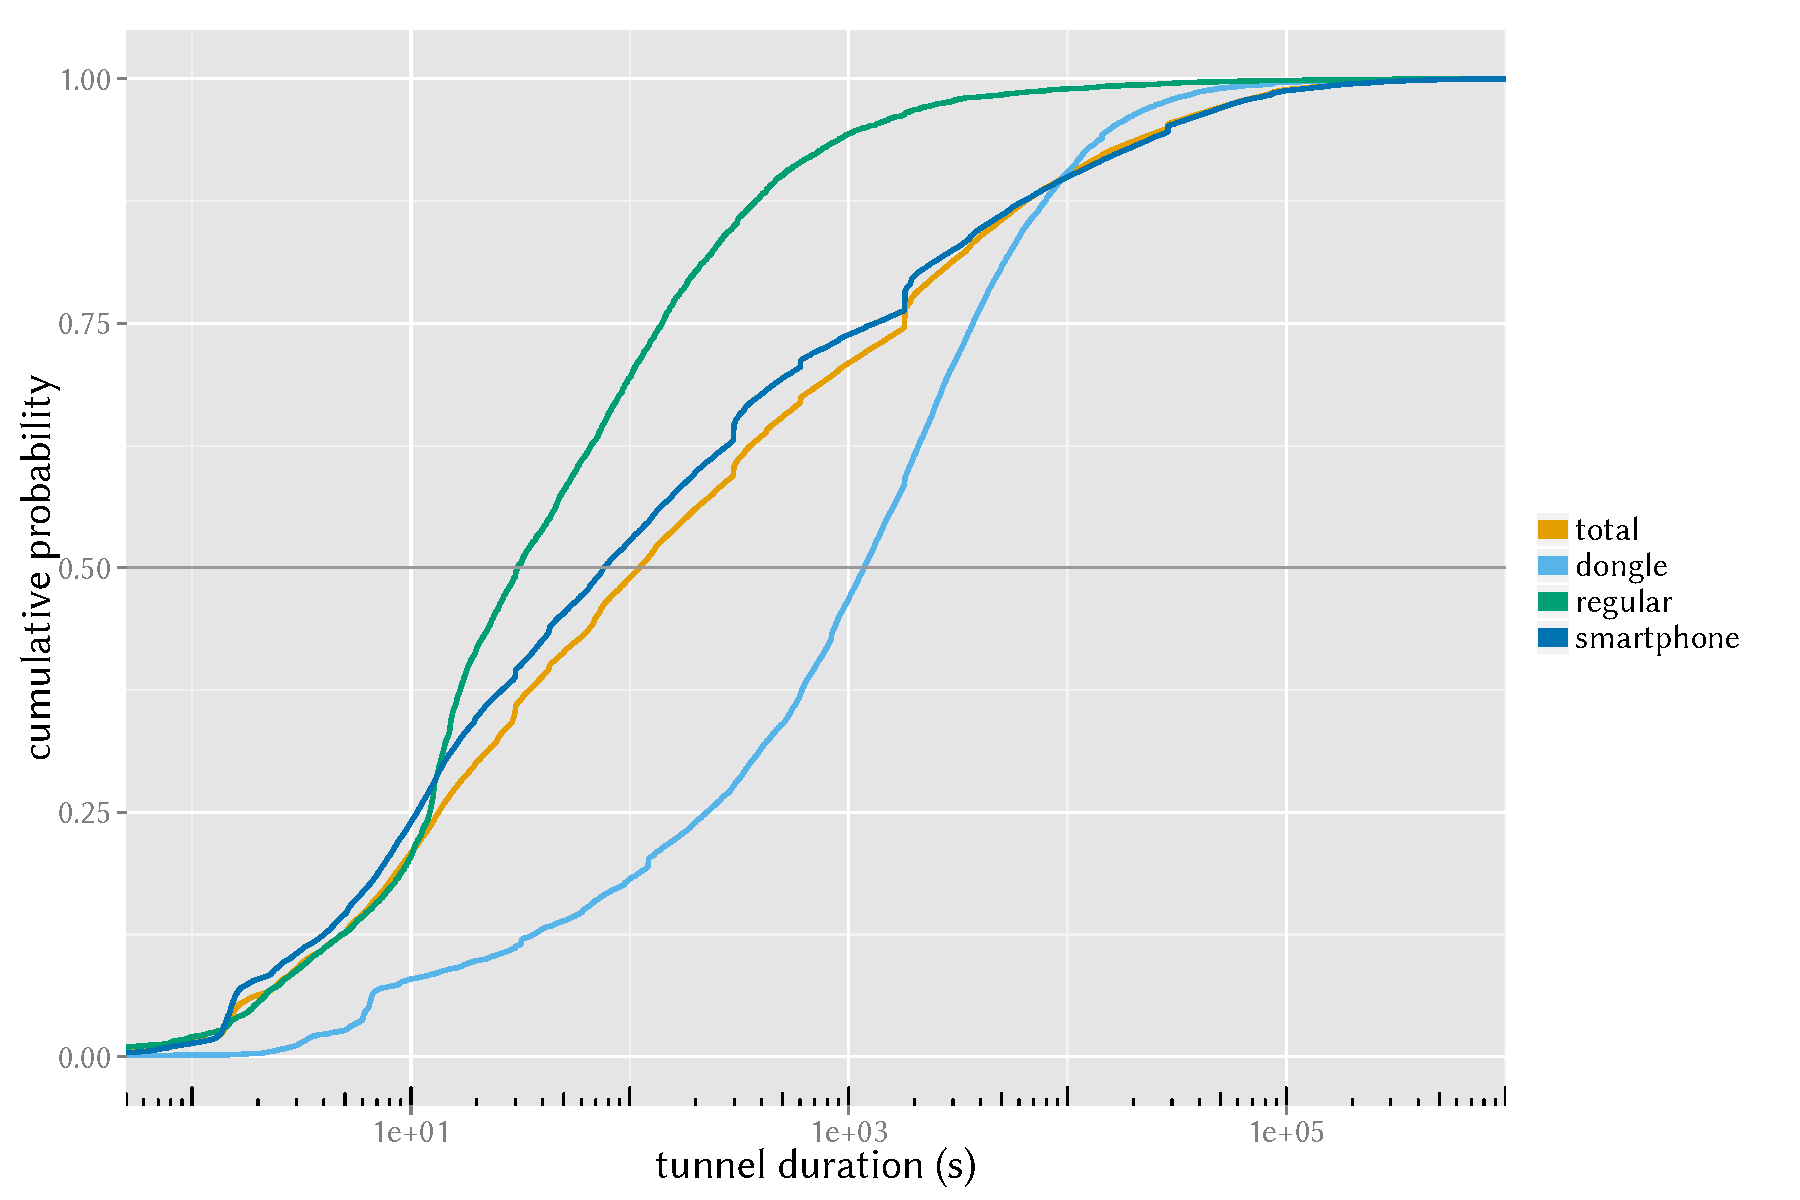
\includegraphics[width=0.9\textwidth]{images/R-tunnel-duration-device-type.pdf}
	\caption{Tunnel duration distribution, separated for \acrshort{3G} dongles, smartphones and regular phones with medians at \SI{115}{\second} (total), \SI{31}{\second} (regular), \SI{82}{\second} (smartphone), and \SI{1207}{\second} (dongle).}
\label{c4:fig:cdf-duration-device-class}
\end{figure}

Figure~\ref{c4:fig:cdf-duration-device-class} shows the \gls{ECDF} for the user tunnels and their \gls{PDP} Context durations in the dataset. In this first graph, the duration of different device classes is distinguished and put in perspective to the overall duration distribution. The devices classes here are smartphones, regular phones, and \gls{3G} dongles. It can be observed that tunnel durations range between seconds and more than one week.

The median can be clearly differentiated between device types, being much longer for \gls{3G} dongles than for mobile phones. This reflects expected user behavior very well and gives a first indicator on a possible influence of the user plane on the control plane.

Dongles are usually used with laptops to be able to work while being mobile. Dongle sessions last therefore often for extended periods longer than a few minutes up to hours. Also, this type of device is usually put into a standby mode after the period, which completely disables any mobile connections --- and therefore any associated tunnel --- instead of switching to low power radio idle modes. This is reflected in the dongle tunnel duration here as well. When compared to the other device category, dongles are more compactly centered around their median of about \SI{20}{\minute}.

A similar behavior can be observed in the regular phone distribution with values arranged tightly around the median of \SI{31}{\second}. Compared to today's smartphones, data connections on regular phones are mostly initiated explicitly by user interaction, for example through starting a browser and viewing a web page. This could also explain the comparatively low durations here.

The picture is rather different in the smartphone tunnel duration. Here, often background tasks are running over long periods of time and devices try to keep connectivity up as long as possible (while still attempting to conserve power). Overall, this could lead to the smoother distribution seen here with no clear center value.

Overall, a relatively high number of tunnels with a duration shorter than \SI{10}{\second} can also be observed. Especially the peak at about \SI{1.5}{\second} --- which is interestingly shifted to \SI{6.8}{\second} in the dongle distribution --- is of note. This is even shorter than the default values for the \gls{RRC} idle state transitions which causes the tunnel to be destroyed. It can be conjectured that these short tunnels have been explicitly removed by the \gls{UE} as no other involved state machine has timers this short.

Another distinct step at \SI{30}{\minute} in the total and smartphone distributions can be observed. As it is only present in these to categories --- and the total distribution looks to be mostly governed by smartphones --- it is reasonable to assume that the cause for this is a specific behavior observable in some aspect of smartphone related influence factors.


%%
\paragraph{Influence of the \texorpdfstring{\acrshort{os}}{OS}}

\begin{figure}[htb]
	\centering
	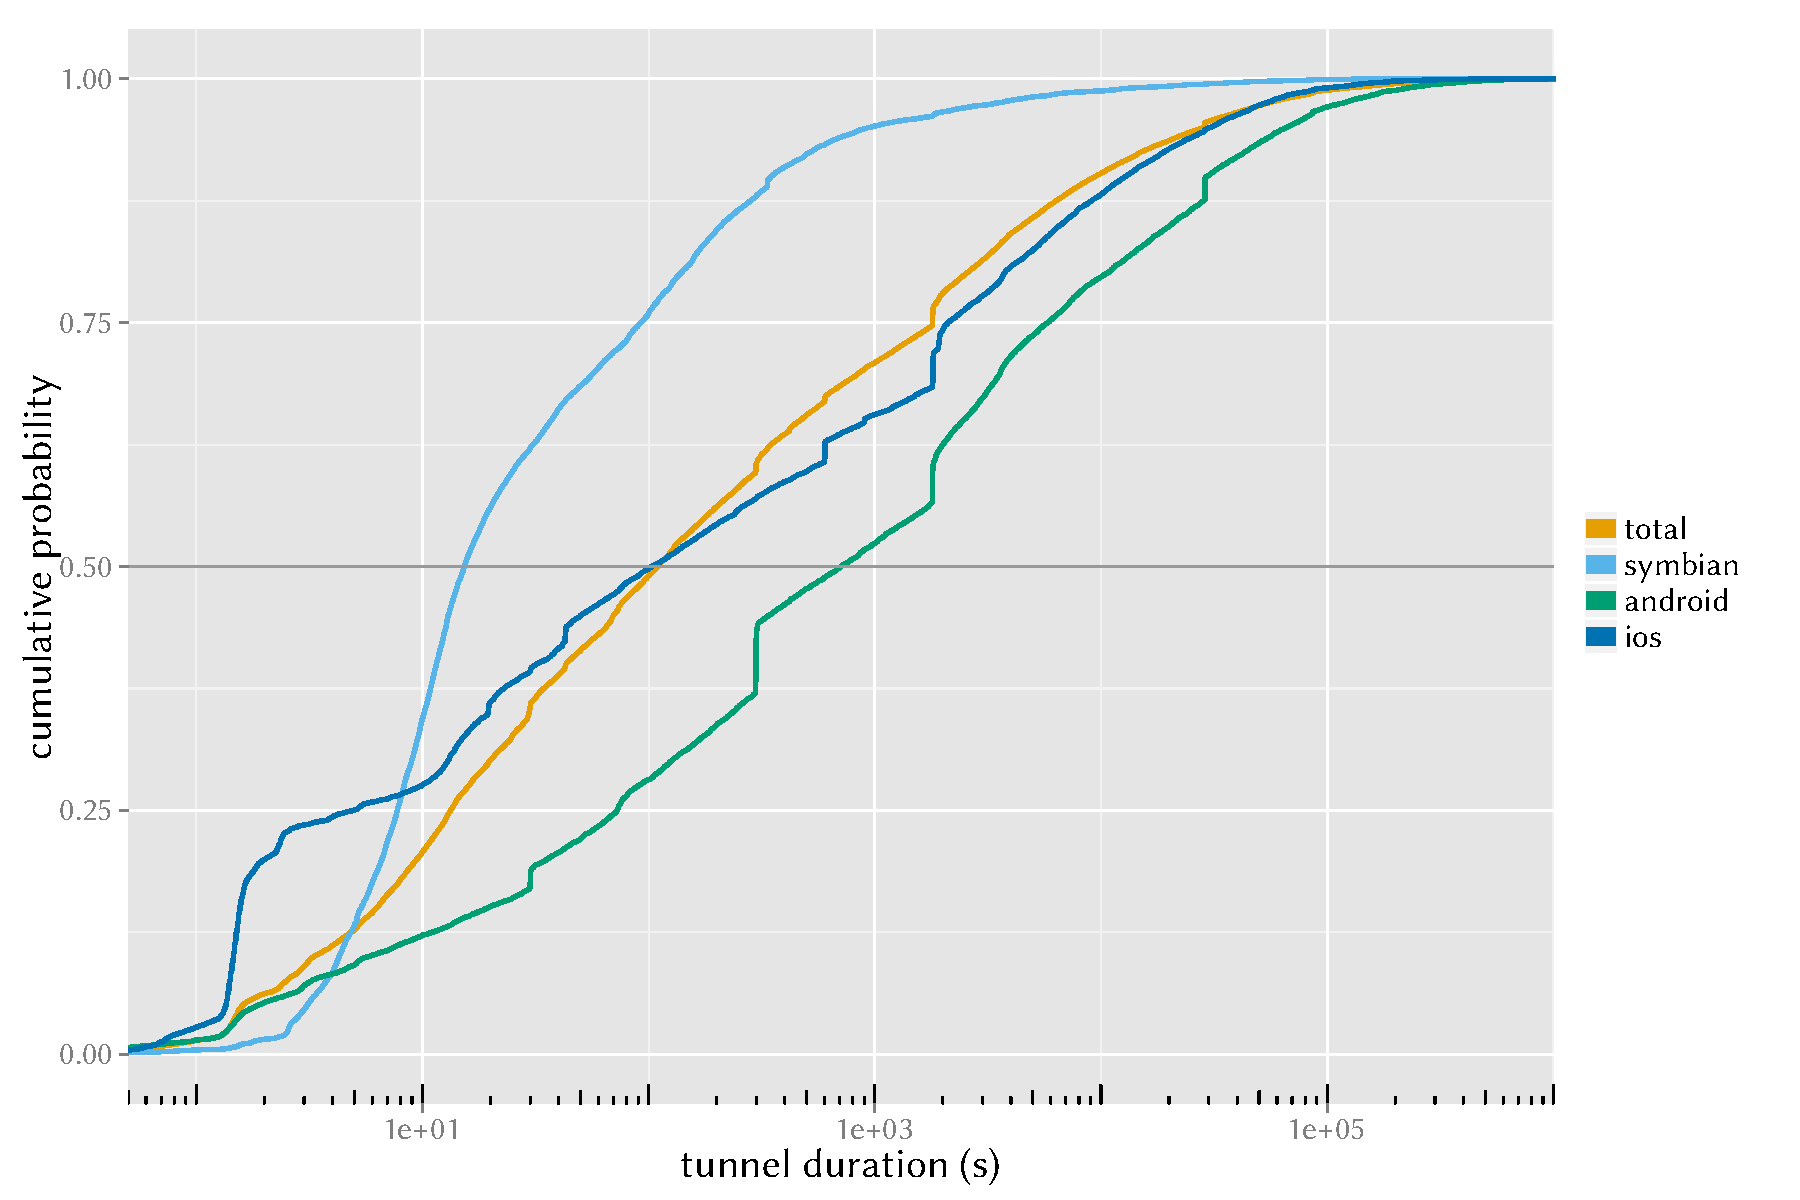
\includegraphics[width=0.9\textwidth]{images/R-tunnel-duration-operating-system.pdf}
	\caption{Tunnel duration \acrshort{CDF}, separated for select \acrshortpl{os}; Medians at \SI{115}{\second} (total), \SI{15.5}{\second} (symbian), \SI{104}{\second} (iOS), and \SI{765}{\second} (android).}
\label{c4:fig:cdf-duration-os}
\end{figure}

Next, the two phone categories are further broken down by their \gls{os}. Only the three major systems, Android, iOS, and Symbian, are identified here, the amount of other types was negligible. The smartphone category is almost exclusively represented by Android and iOS devices, while Symbian devices make up most of the regular phones but is also represented in a number of smartphone models.

Figure~\ref{c4:fig:cdf-duration-os} depicts the \gls{ECDF} of the tunnel durations of these categories in relation to the total duration distribution. They immediately exhibit a clear difference between individual \glspl{os}.

The Symbian tunnel durations are similarly distributed to the previously depicted regular phone category, albeit with an even shorter duration median of about \SI{15}{\second}. This is an indicator of the large intersection between these two groups and the explicit user traffic property attributed to regular phones.

The two smartphone-exclusive \gls{os} have remarkably similar tunnel distributions with the exception of the Android tunnel distribution shifted to much longer tunnels. This is mostly due to the larger accumulation of iOS tunnels around the previously mentioned \SI{1.5}{\second} mark. Over \SI{20}{\percent} of all tunnels established by iOS devices are shorter than \SI{2}{\second}. A possible explanation is an interaction between the described implicit background traffic happening in intervals and the efforts of iOS phones to preserve as much energy as possible. 

To this end, phones aggressively force their radio connection to the low power idle states or even completely shut off the radio immediately after transmission have ended, circumventing \gls{RRC} timers. To achieve this, iOS devices are known to implement a form of \gls{3GPP} Fast Dormancy~\cite{gsma2011fdbestpract}. It is deemed to improve device battery life, radio signaling and radio spectrum efficiency. Due the more frequent state transitions it also could cause an increase in core network tunnel management signaling, which is probably what happened in the iOS case depicted in the \gls{ECDF}.

Another set of tunnel duration accumulations are also visible in the \gls{os} distributions. Two types of steps should be distinguished here. First are accumulations that occur across multiple or all categories. This points to an influence source outside of the specific category. If the artifact is present in every distribution it is even likely that the source is a behavior of the network's state machines. The second type of accumulation is local to one or some categories, which places the root cause into the region of these categories and their related influence factors. 

In case of the \gls{os} category, additionally, peaks at \SI{30}{\second}, \SI{300}{\second}, and \SI{600}{\second} can be observed. However, whether this behavior can be attributed directly to the operating systems themselves cannot be decided just by looking at these distribution. Other factors, e.g., the device's baseband and user traffic dynamics, also play a role. 


%%
\paragraph{Influence of the Time of Day}

\begin{figure}[htb]
	\centering
	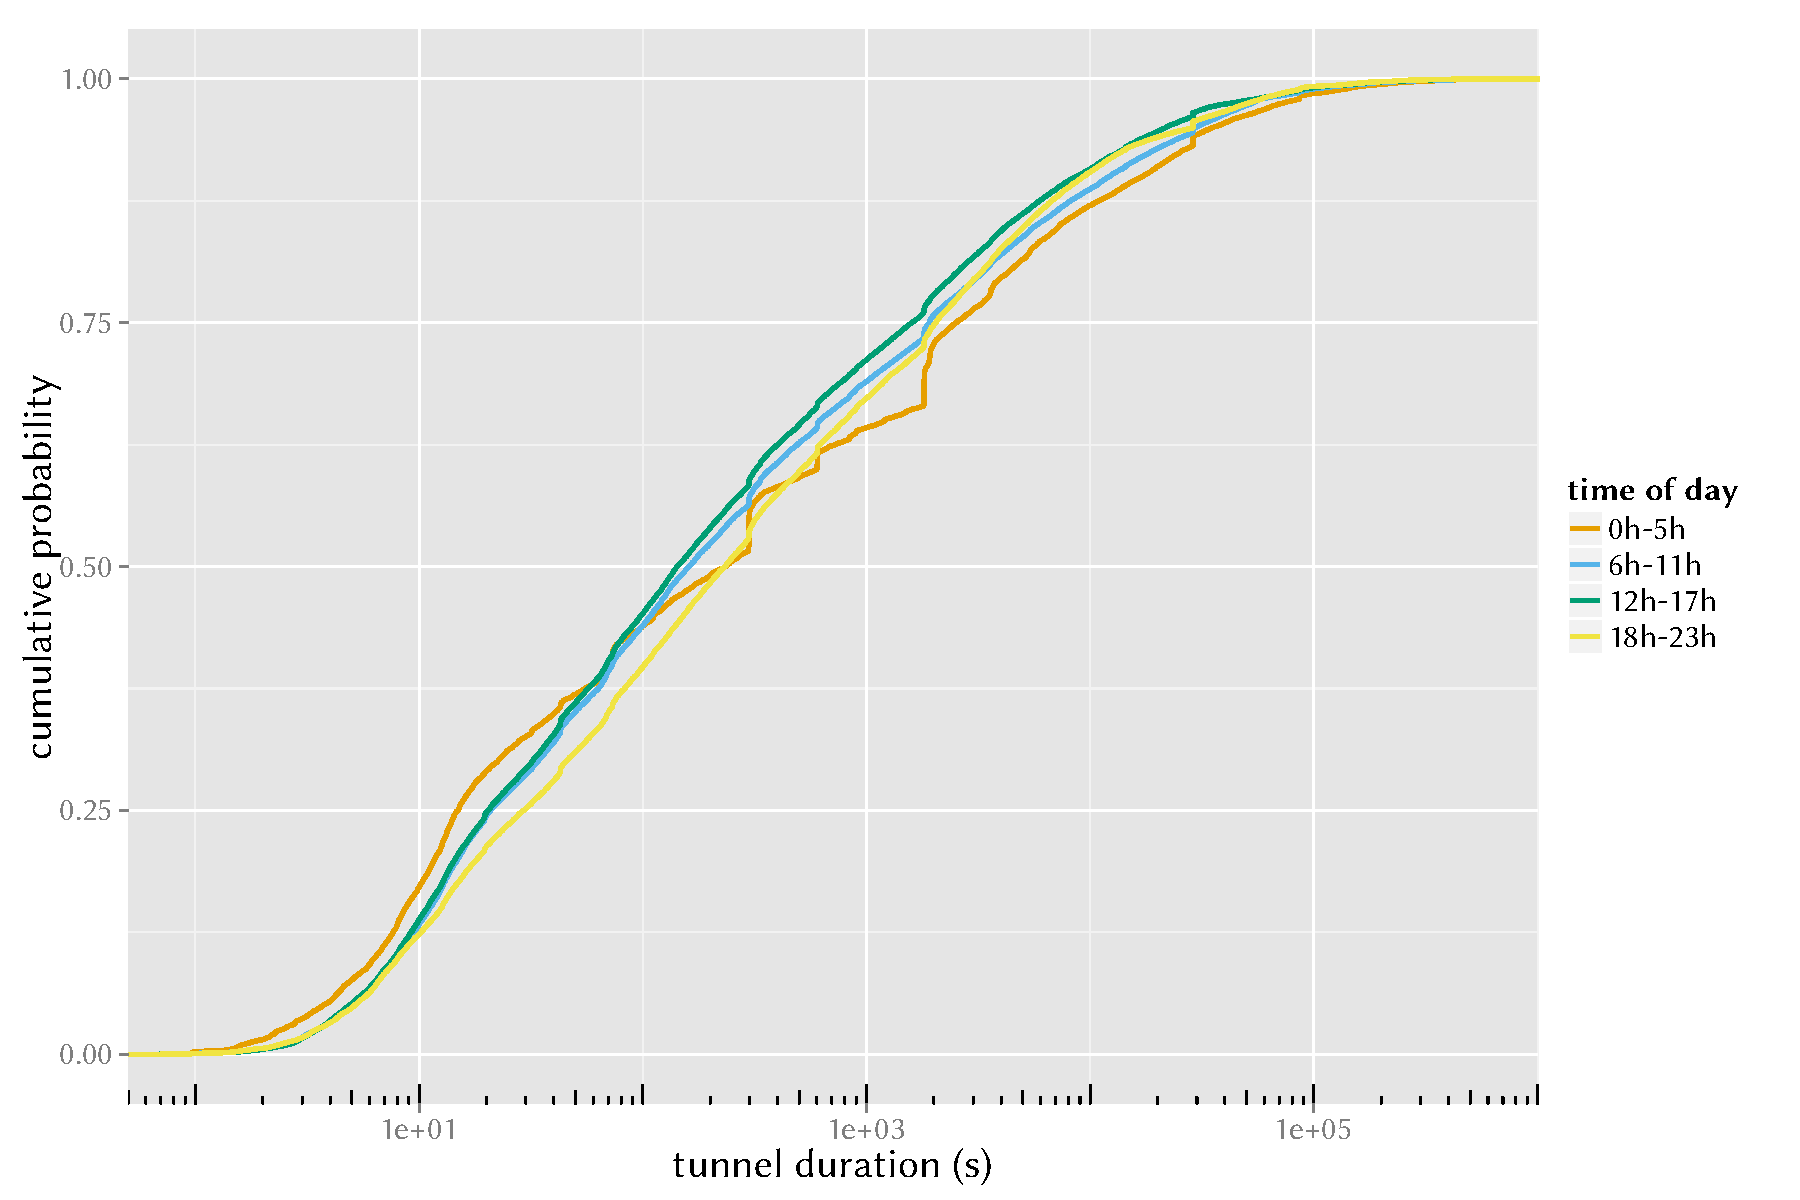
\includegraphics[width=0.9\textwidth]{images/R-duration-timeofday-ecdf.pdf}
	\caption{Tunnel duration of all active tunnels by time of day.}
\label{c4:fig:duration-timeofday-ecdf}
\end{figure}

In addition to device factors, diurnal effects could also play a role in the duration of tunnels. Figure~\ref{c4:fig:duration-timeofday-ecdf} depicts $24$ individual \glspl{ECDF} of the tunnel duration for each hour of a day. While no clear distinctions are visible, there is a trendto shorter tunnels in the early morning hours. The early afternoon hours tend to produce tunnels more centered around the middle duration range. Even longer tunnels should be treated with reservation, as they exceed the length of their assigned time slot in the \gls{ECDF} and span a larger time frame. Only the tunnel creation point is guaranteed to be in the slot.


%%
\paragraph{Influence of Other Factors}

Due to the nature of the trace dataset at hand many other influence factors are hard or outright impossible to distinguish. Some factors are unknown from the \gls{CN} perspective, as the mentioned device baseband, while others have not been recorded in the trace.

For example, it would theoretically be possible to investigate the influence of the \gls{RAT} as it is an \gls{IE} in the \gls{gtp} messages and also recorded in the trace. The radio access parts of \gls{GSM} and \gls{UMTS} are completely different --- including the \gls{RRC} state machines which were depicted in Figure~\ref{c4:fig:mmstatemodel} --- and therefore could also differ in their control plane load impact on the core. However, the \gls{RAT} \gls{IE} is optional and only set in less than \SI{1}{\percent} of the available records. As the radio access can change even during an existing tunnel --- in which case the \gls{GGSN} receives a \gls{gtp} update request informing the node about the change --- a complete picture without gaps would be required to do any investigation on this.


%%
\paragraph{Influence Strength of the Categories}

\begin{figure}[htb]
	\centering
	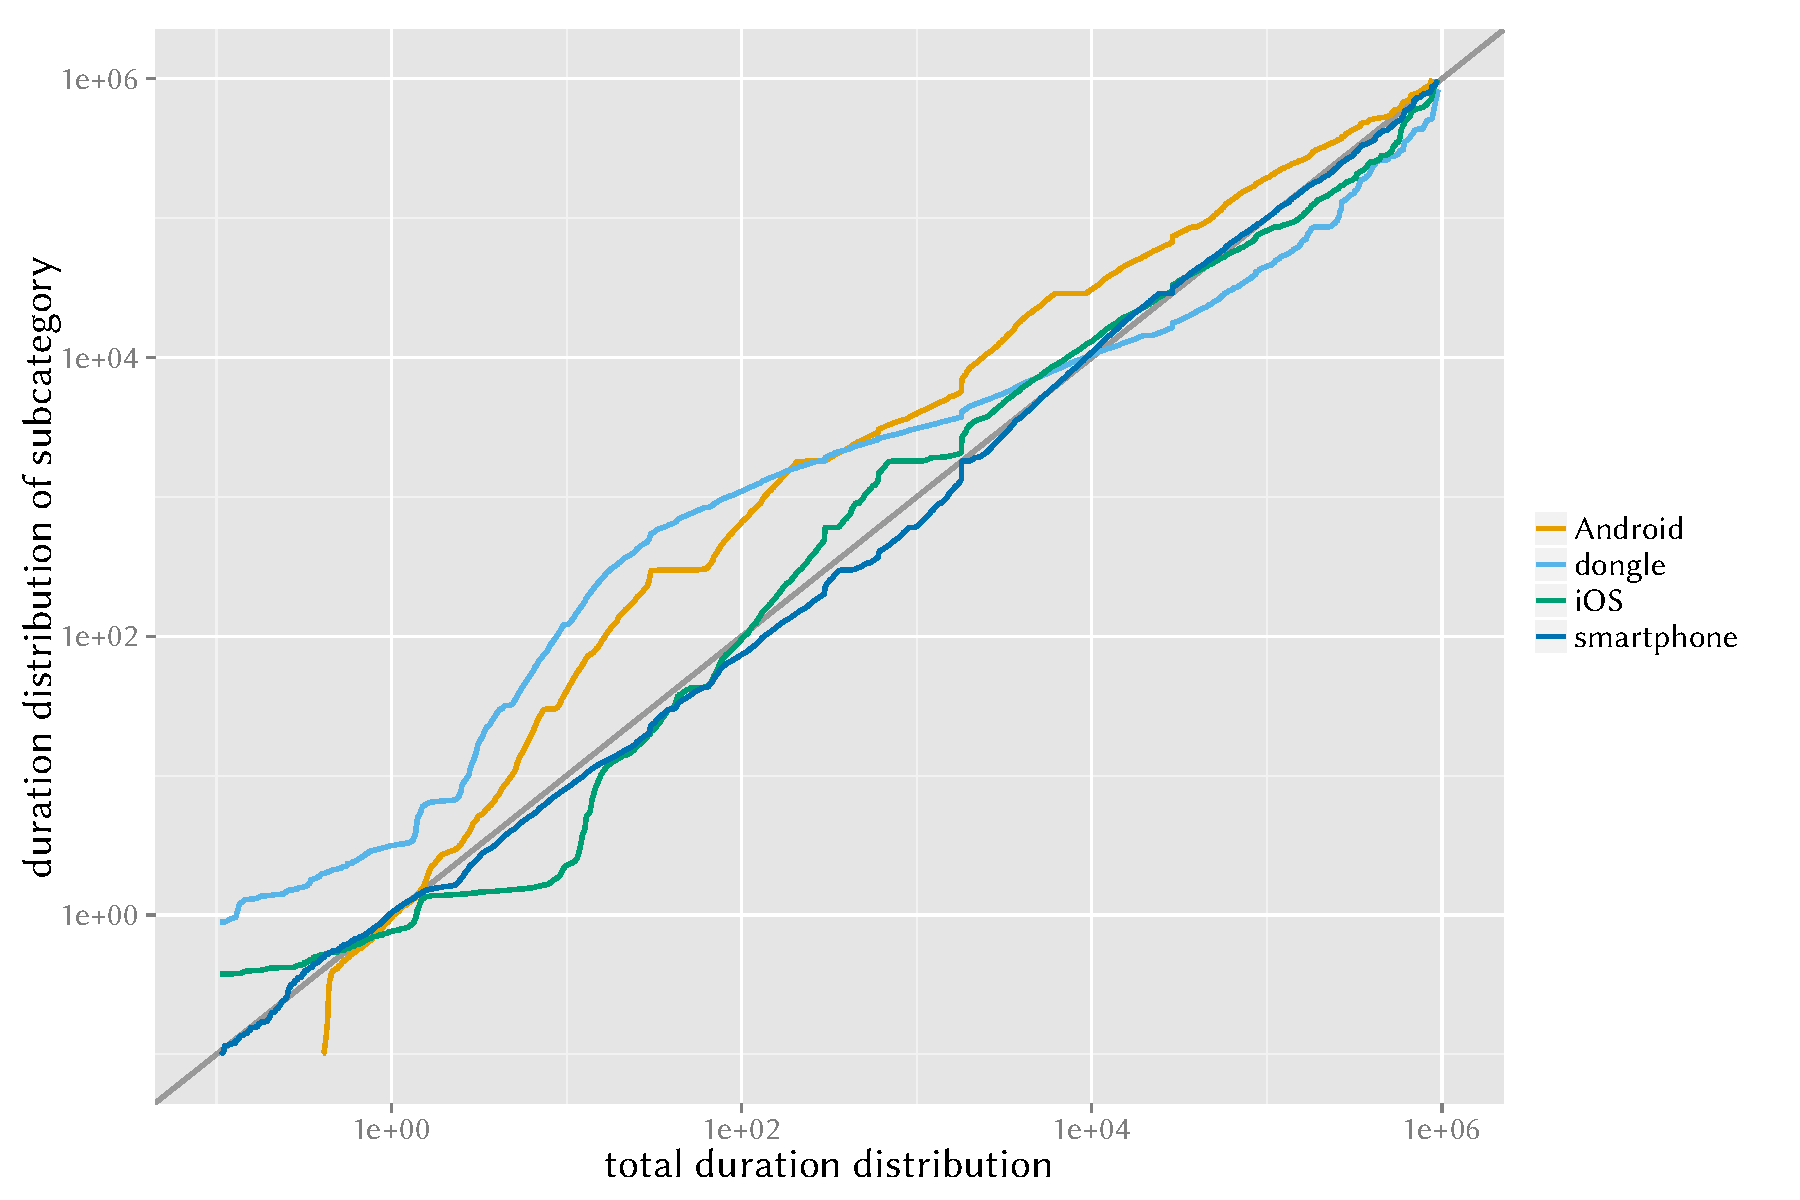
\includegraphics[width=0.9\textwidth]{images/R-duration-qq-category-comparison.pdf}
	\caption{Q-Q Plots of the tunnel duration distributions in comparison to device classification categories.}
\label{c4:fig:qq-plots}
\end{figure}


To ascertain which of the investigated device categories influences the total duration distribution most, Q-Q plots are created and investigated. It is conjectured that the amount of influence on the duration distribution is correlated to the influence on the control plane load. In theory, if both durations follow the same distribution, one expects a straight diagonal $y=x$ line through the origin. A steeper incline indicates more compact regions in the distribution plotted on the $x$ axis and vice versa.

The Q-Q plots in Figure~\ref{c4:fig:qq-plots} compare the total tunnel duration distribution to the duration distribution of the dongle, smartphone, Android, and iOS classification cateogries. It can be observed that the smartphone duration distribution is distributed almost equally to the total except for minor variations. However, the \gls{3G} dongle tunnel durations follow a very different distribution. Their effect on the total duration distribution seems to be negligible despite the  large amount of traffic they are causing. This is also a first indicator that smartphones might have a larger impact on signaling than other device types.

Looking closer at the smartphone category, Q-Q plots of the two major \glspl{os} are investigated. With the exception of the large below \SI{2}{\second} peak in the lower tail of the distribution, iOS device tunnel durations are very similar to the overall tunnel duration distribution. The same can not be said about the Android distribution, which deviates somewhat in the distribution's center but is similar to the total distribution in the upper tail. Even devices with just a different \glspl{os} seem to strongly differ in their influence on duration distribution and therefore on signaling.

\begin{figure}[htb]
	\centering
	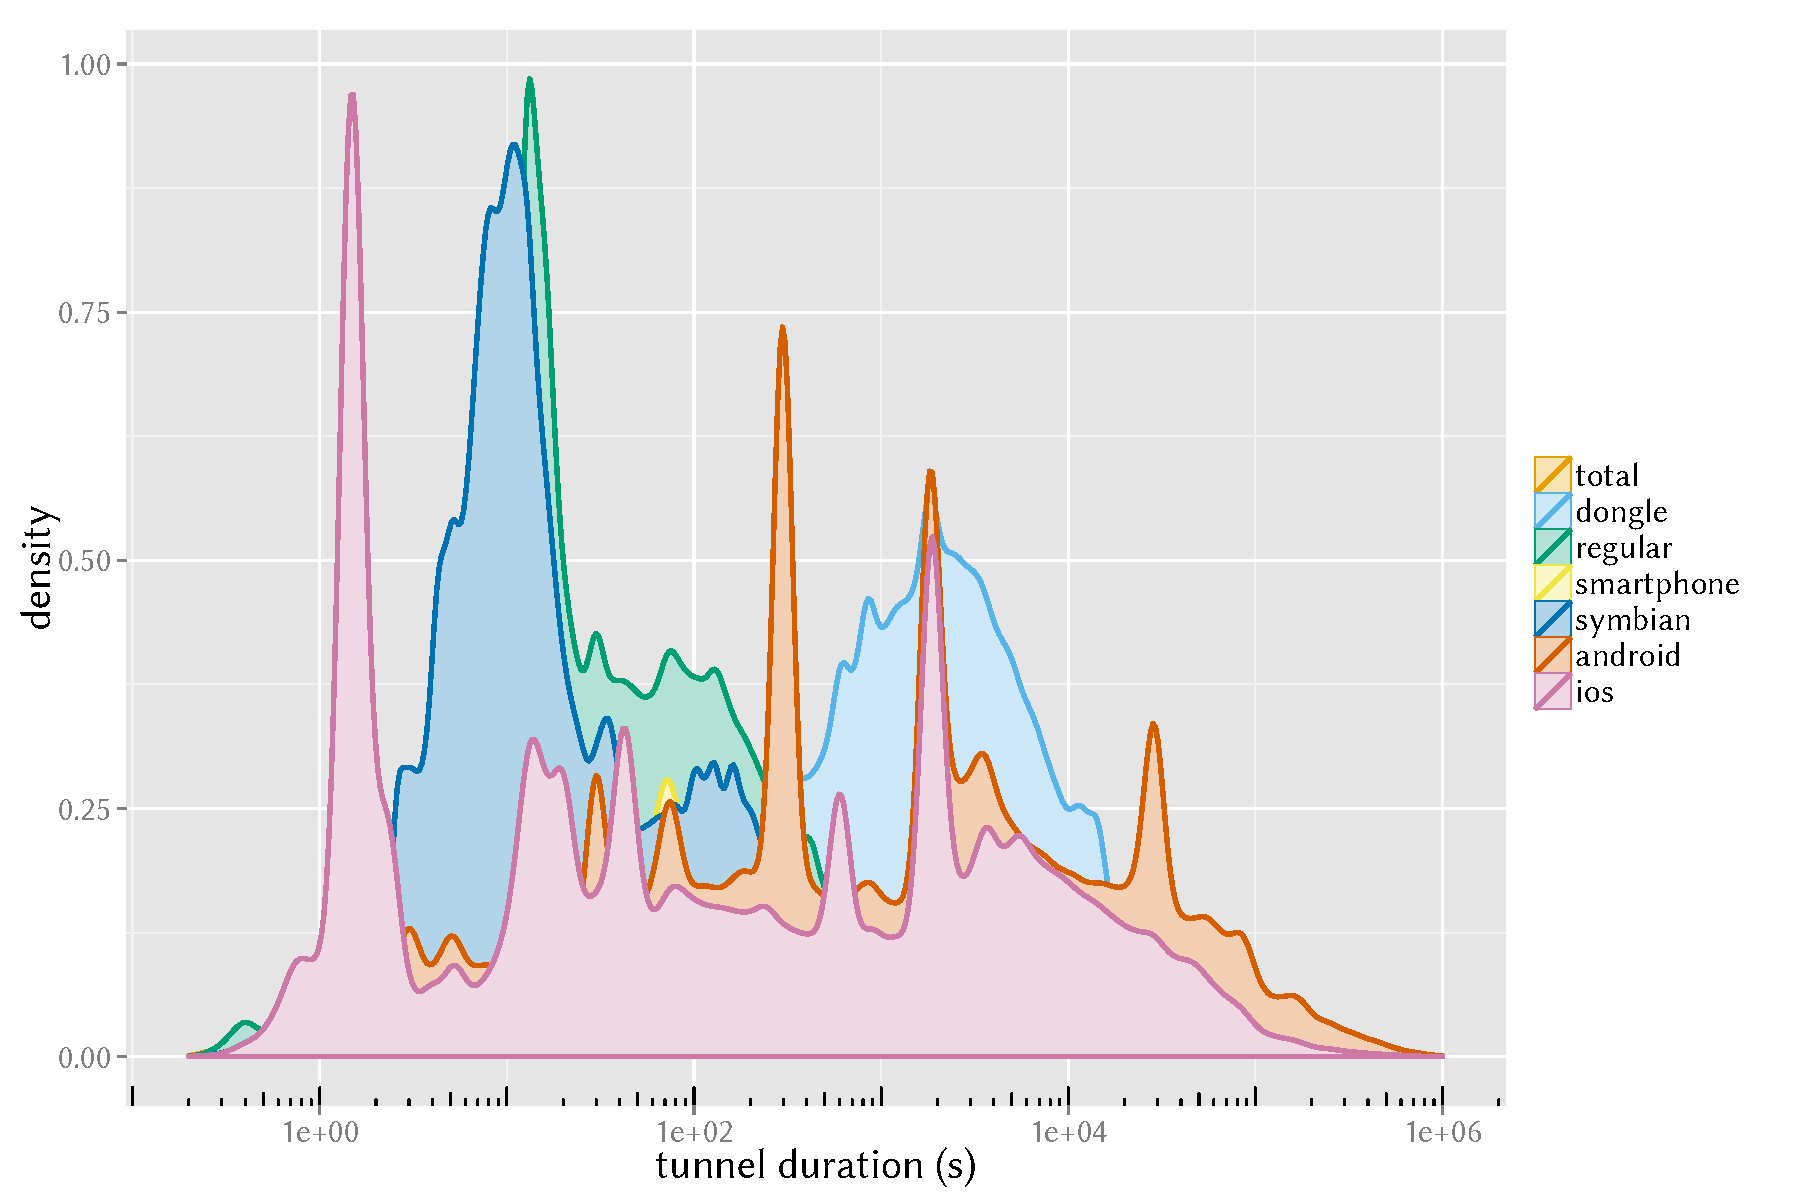
\includegraphics[width=0.9\textwidth]{images/R-duration-classification-density.pdf}
	\caption{Logscale density plot of the tunnel duration with all classifications.}
\label{c4:fig:durations-density}
\end{figure}


Figure~\ref{c4:fig:durations-density} attempts to depict where in their distributions the investigated device categories show the most impact on the total distribution. The plot shows the density of all previously investigated device influence categories.

It is evident that the durations are not evenly distributed, but rather follow sharp spikes. One of largest spike across all categories is the one at a duration of \SI{30}{\minute}, with about \SI{1.8}{\percent} of all tunnels in the network falling into that region. Since this spike happens across all device types, it makes a rather strong case for being induced by the network. On the other hand, the bulk of tunnel durations in the short-to-medium range does not seem to be governed by the two major smartphone operation systems but by other devices in the network, which do not show major spikes in other bins.

Besides the long-tailed behavior in the upper tail of the tunnel durations another slight accumulation effect, repeating itself every \SIrange{6}{7}{\day}, is present in the upper tail. This phenomenon is as yet of unknown origin and does not coincide with any known timers of the \gls{3G} mobile network.

The investigation of this data leads to the conclusion that the planning and dimensioning of the control plane needs to watch the behavior of smartphones more carefully than that device types.


%%%%%%%%%%%%%%%%%%%%%%%%%%%%%%%%%%%%%%%%%%%%%%%%%%%%%%%%%%%%%%%%%%%%%%%%%%%%%%%
\subsubsection{\texorpdfstring{\acrshort{gtp}}{GTP} Tunnel Arrivals}

The duration of \gls{gtp} tunnels is but one aspect of influence on control plane load. The arrival process of these tunnels is also interesting in itself. Specifically, this mean the arrival of tunnel requests, i.e.\gls{gtp} create requests, at the \gls{GGSN}. 

An arrival process can be described in two distinct ways. First by the number of arrivals in a given time interval. Second, by the \gls{IAT}, the time between two consecutive tunnel arrivals. Depending on the choice one has to deal with either a discrete or a continuous distribution.

Here, the tunnel arrival process is investigated with both approaches. This also adds to the foundation of the load model constructed in the next chapter. Note, that the notion of classifying arrivals into influence categories based on device specifics is omitted here. An investigation of this process can not be realistically be conducted categorized and still relate to the total system load.

\begin{figure}[htb]
	\centering
	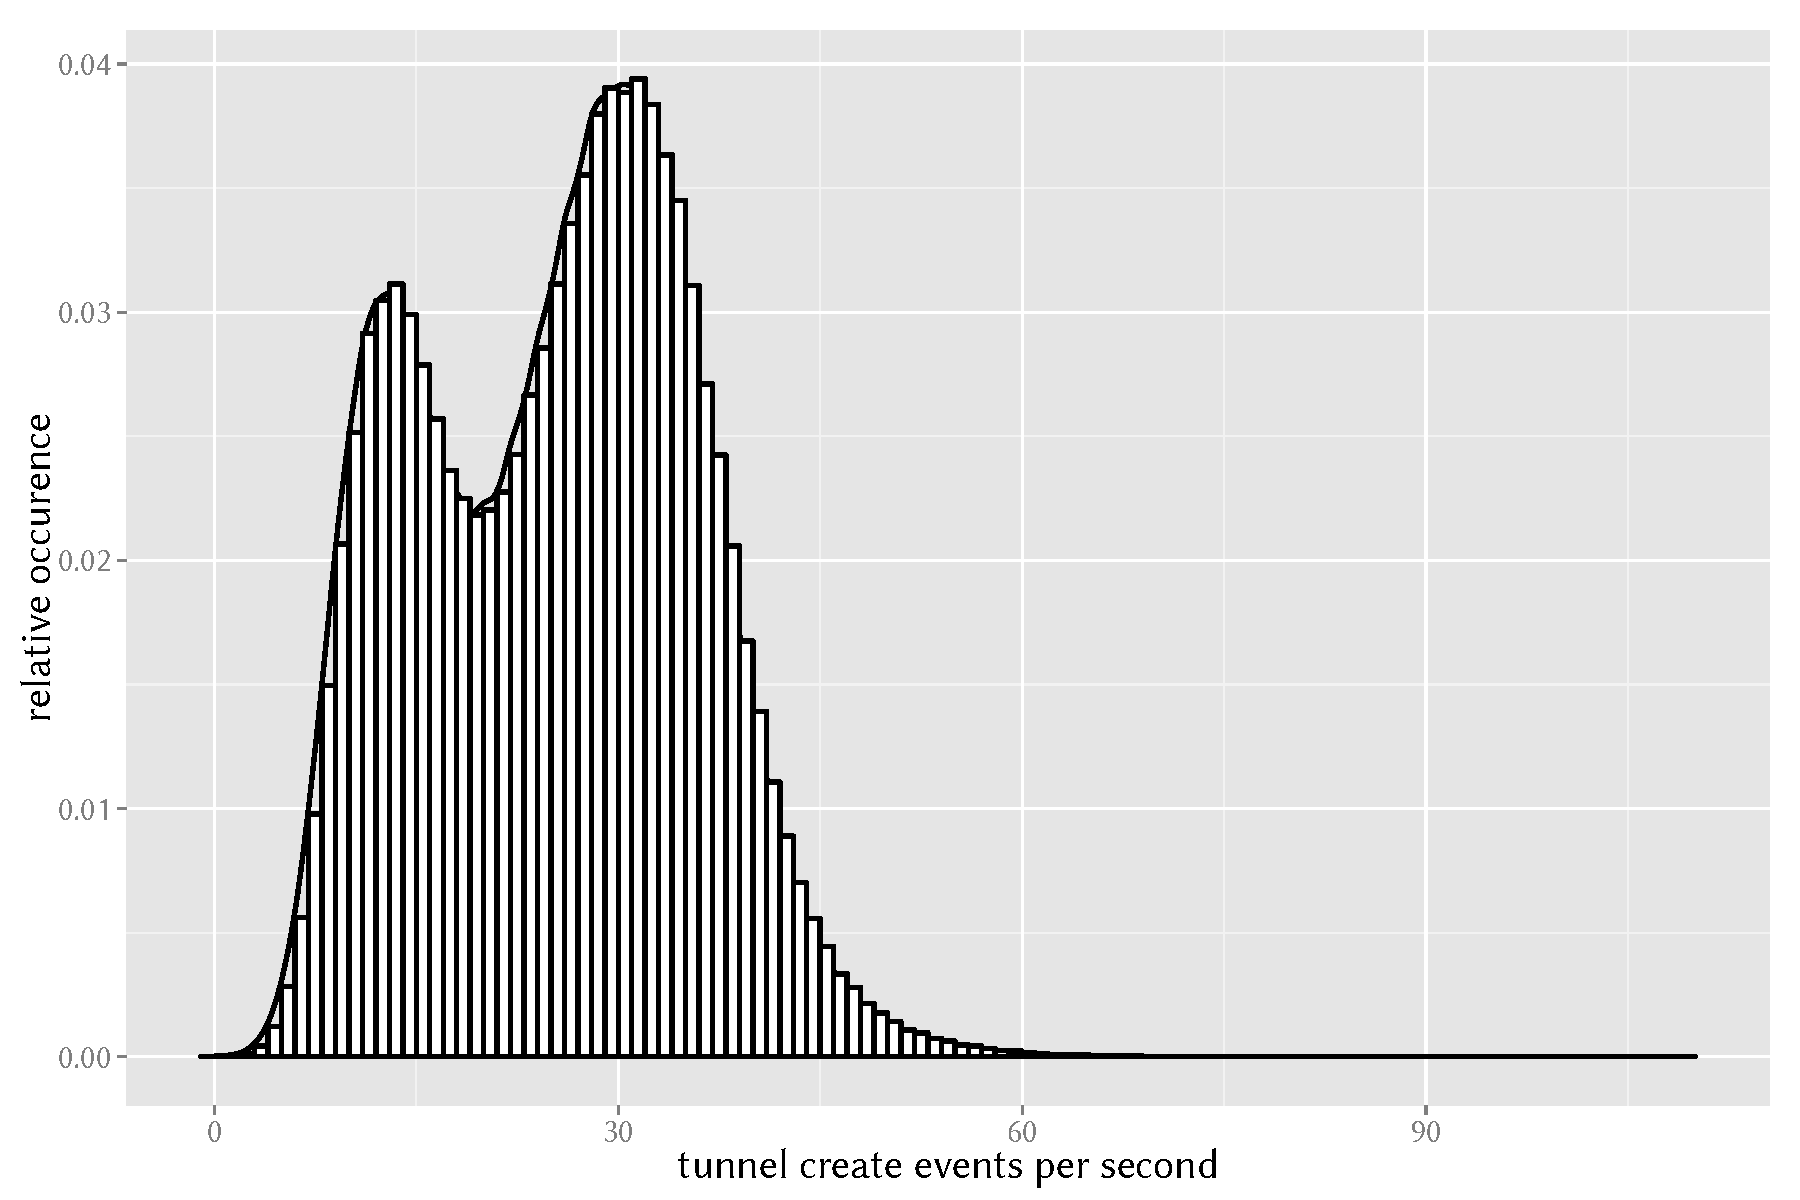
\includegraphics[width=0.9\textwidth]{images/R-create-frequency.pdf}
	\caption{Tunnel arrivals histogram overlaid with a density plot.}
\label{c4:fig:freq-arrivals}
\end{figure}

Figure~\ref{c4:fig:freq-arrivals} depicts a histogram the number of tunnel arrivals per second during the whole trace duration period. Of note is the clear bimodal nature with one peak around twelve and the other in the low thirties. While the distribution is rather compact around these two peaks, there are some clear outliers peaking at $107$ arrivals per second. If the hypothesis of the correlation between signaling load and number of arrivals holds, it can be assumed that load is not constant but rather switches between two modes with some periods of very high load induced by an increased number of arrivals.

\begin{figure}[htb]
	\centering
	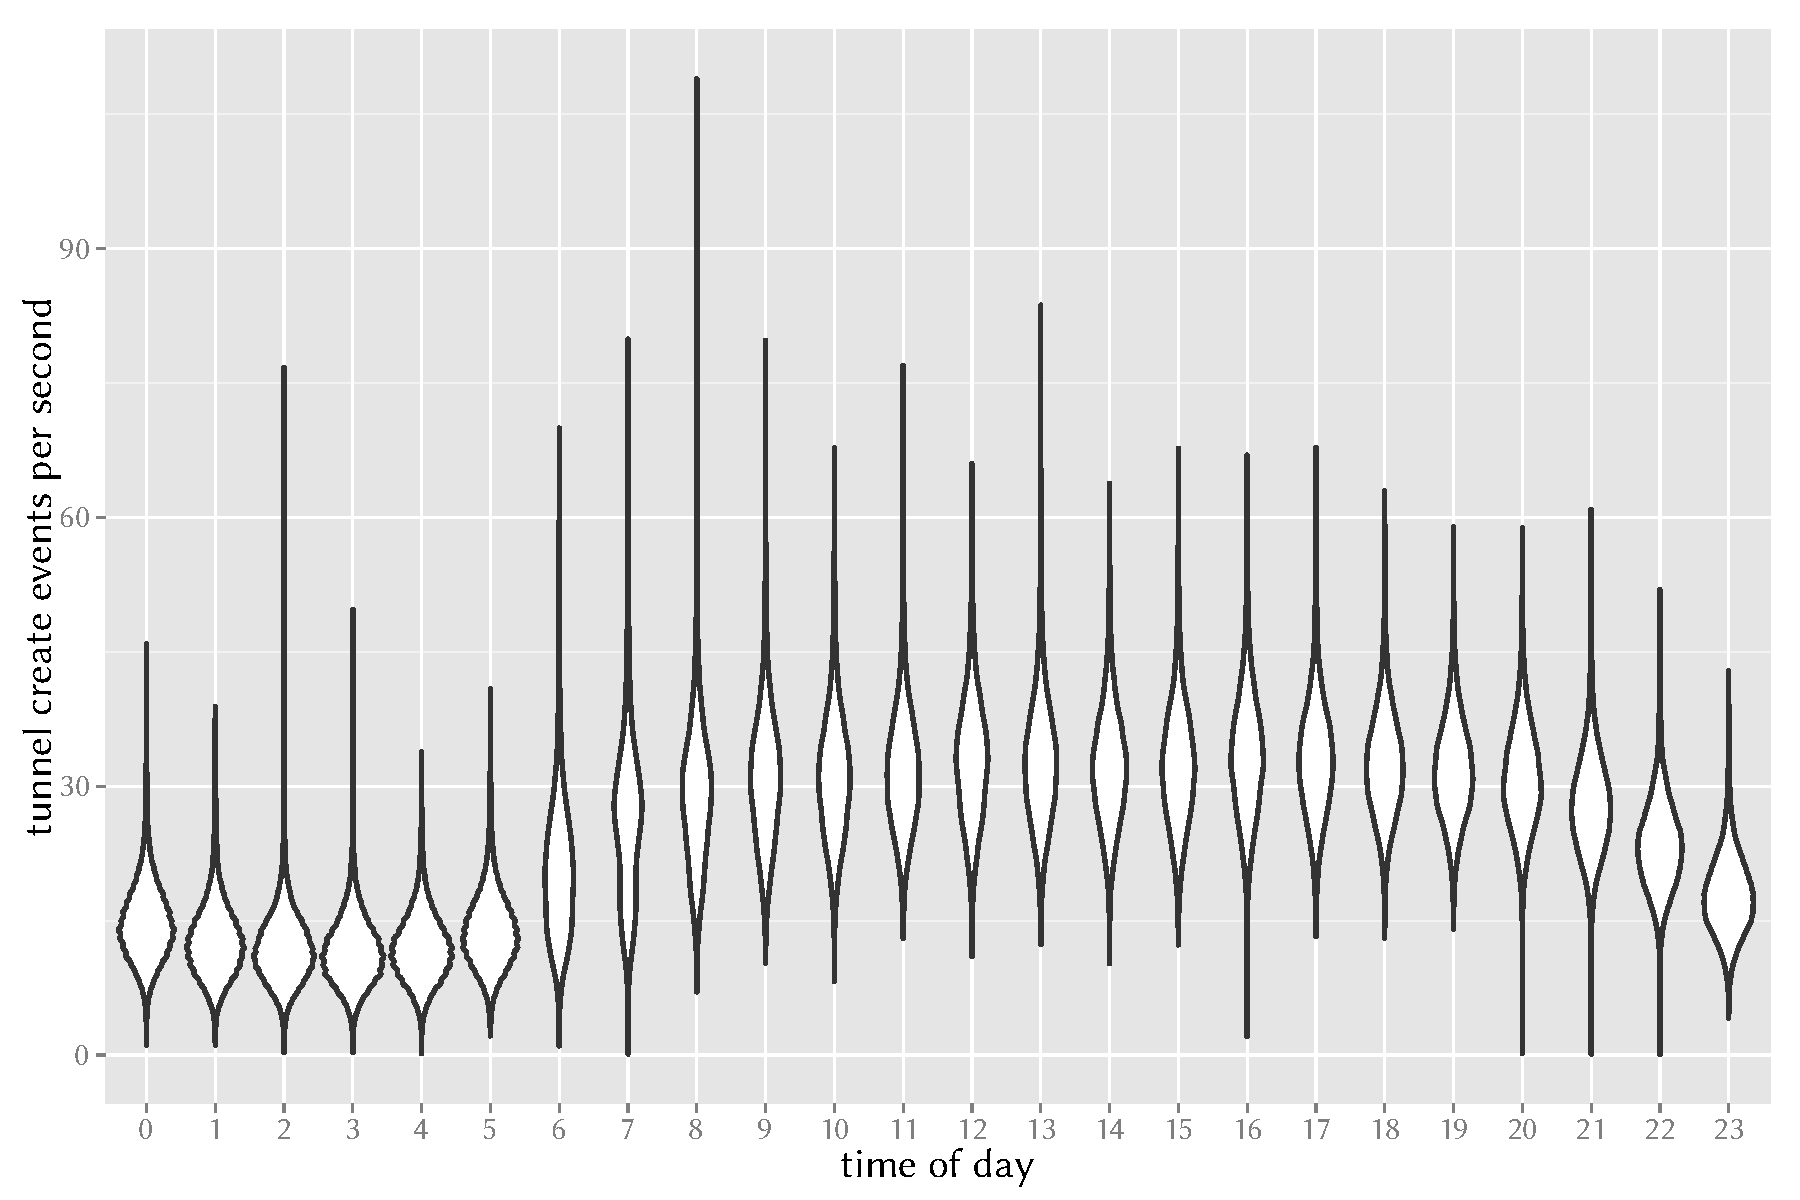
\includegraphics[width=0.9\textwidth]{images/R-createspersecond-1h-violin.pdf}
	\caption{Violin plot of tunnel arrivals in one second per time of day.}
\label{c4:fig:freq-arrivals-per-second-violin}
\end{figure}

A reasonable cause for the occurrence of these two modes can be found in the diurnal arrival patterns. Figure~\ref{c4:fig:freq-arrivals-per-second-violin} contains a violin plot of the tunnel arrivals. This type of plot is similar to a box plot but additionally shows the density of the individual items on the vertical axis. Here the arrivals are broken down to hourly slots. 

The nocturnal plateau of arrivals between midnight and \formattime{5}{0}{0} and the longer daytime plateau between \formattime{8}{0}{0} and \formattime{19}{0}{0} match the two modes found in the histogram. In between are short transition phases. The density of the arrivals during daytime indicates a spread of the number of arrivals over a larger range. This could be an indication of load fluctuations in the system.

\begin{figure}[htb]
	\centering
	\begin{subfigure}[b]{0.5\textwidth}    
		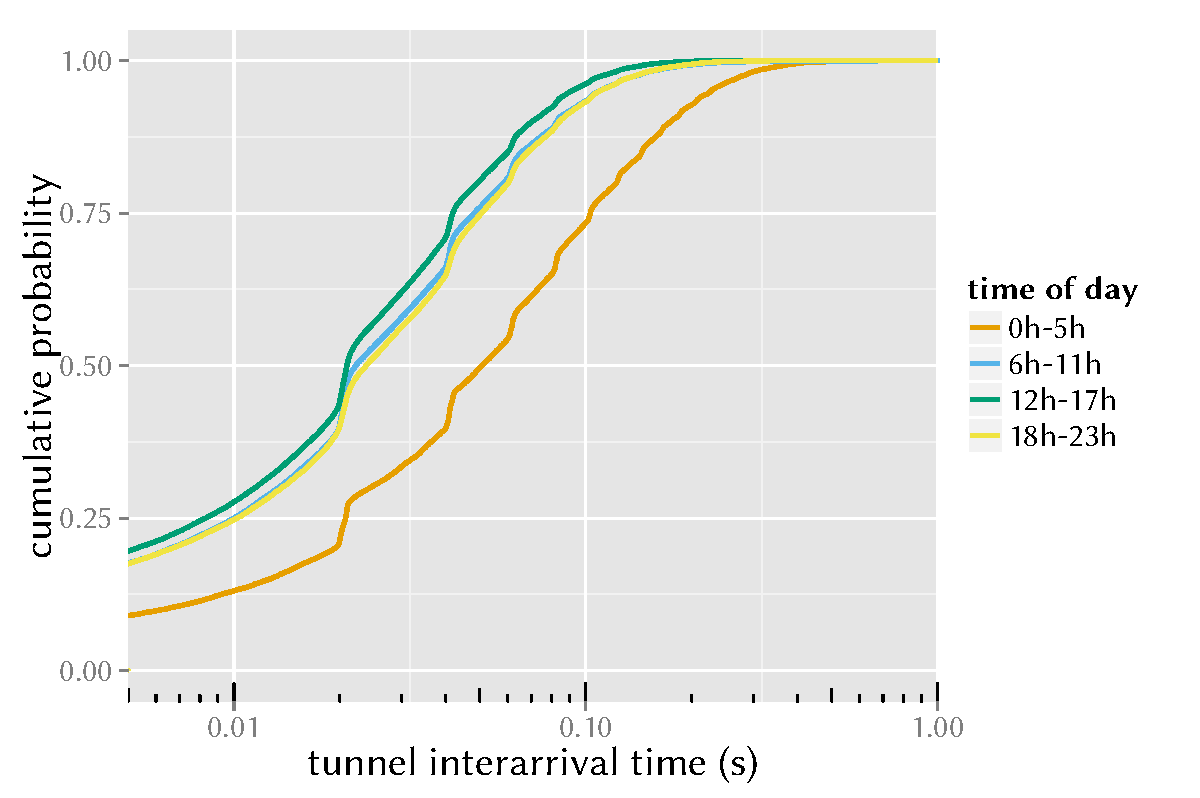
\includegraphics[width=\textwidth]{images/R-IAT-successful-2h-ecdfs.pdf}
		\caption{All tunnel requests.}
		\label{c4:fig:IAT-ecdf-2h-successful}
	\end{subfigure}%
	~
		\begin{subfigure}[b]{0.5\textwidth}
		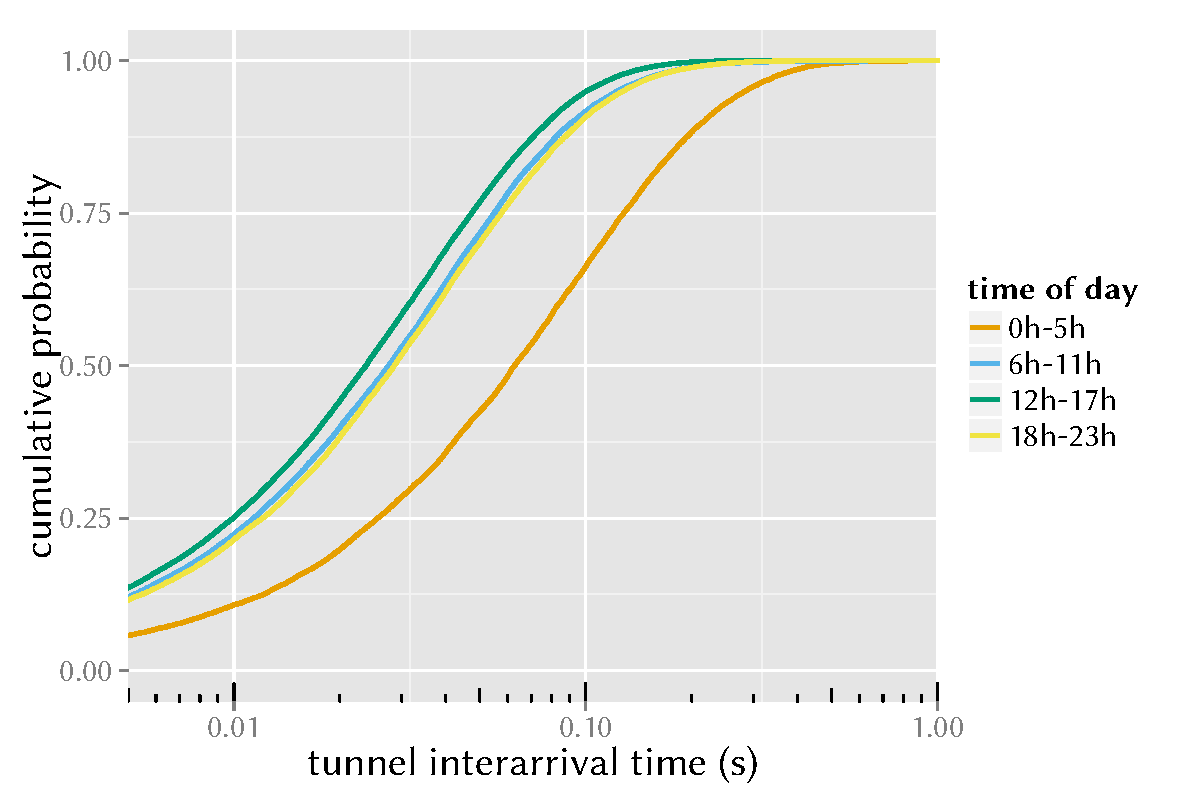
\includegraphics[width=\textwidth]{images/R-IAT-fromflows-ecdfs-2h.pdf}
		\caption{Only tunnels with data flows.}
		\label{c4:fig:IAT-ecdf-2h-active}
	\end{subfigure}

	\begin{subfigure}[b]{0.5\textwidth}
		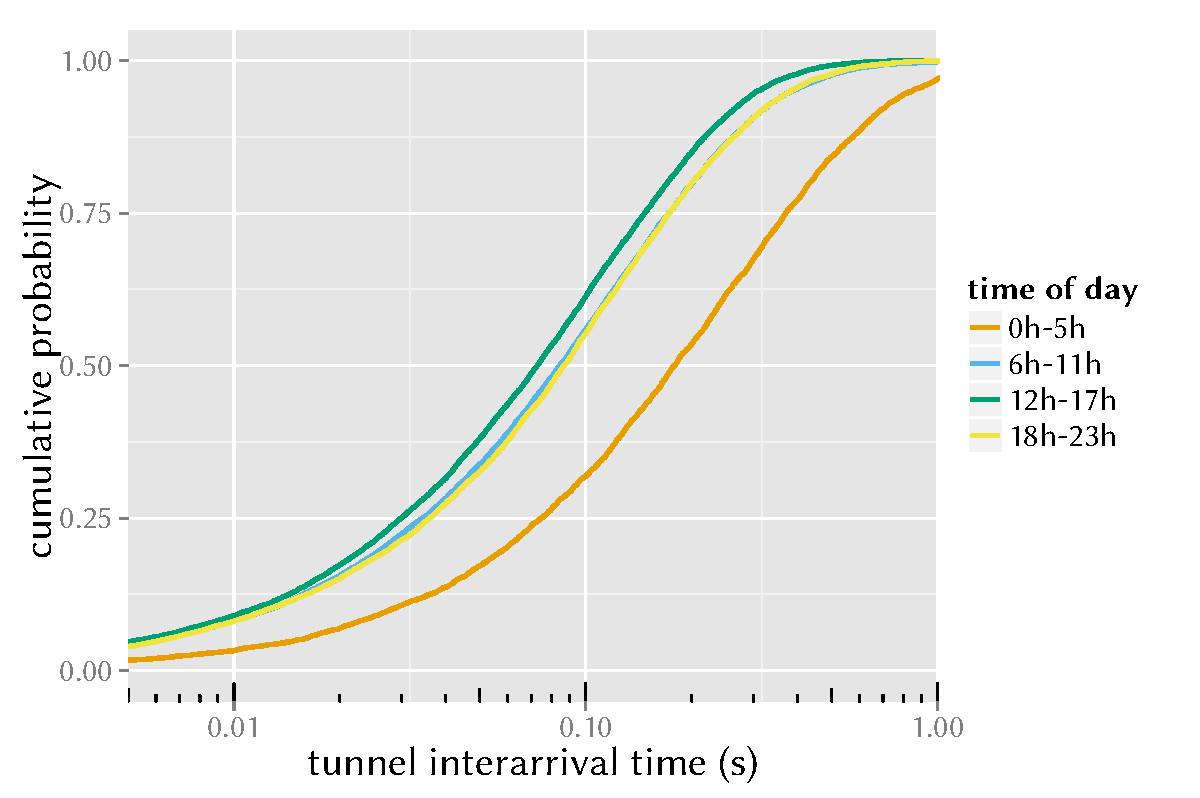
\includegraphics[width=\textwidth]{images/R-IAT-fromflows-gprs-ecdfs-2h.pdf}
		\caption{Tunnels with data flows initiated in \gls{GPRS}.}
		\label{c4:fig:IAT-ecdf-2h-active-gprs}
	\end{subfigure}%
	~
	\begin{subfigure}[b]{0.5\textwidth}
		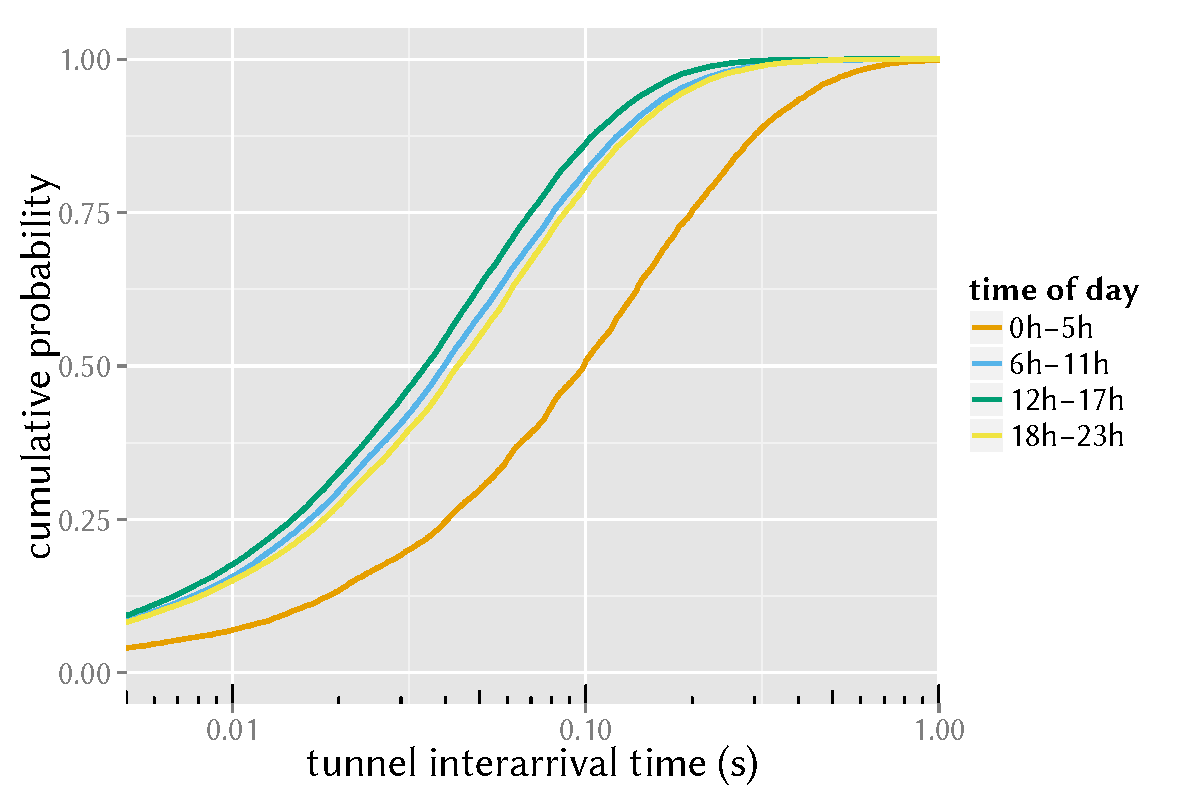
\includegraphics[width=\textwidth]{images/R-IAT-fromflows-umts-ecdfs-2h.pdf}
		\caption{Tunnels with data flows initiated in \gls{UMTS}.}
		\label{c4:fig:IAT-ecdf-2h-active-umts}
	\end{subfigure}
	\caption{\acrshortpl{ECDF} of the tunnel \acrshort{IAT} in seconds by time of day.}
\label{c4:fig:IAT-ecdf-2h}
\end{figure}

Complementing the arrival rate evaluation is the investigation of the tunnel \gls{IAT}. This metric is more sensitive to short time fluctuations of arrivals and more suited to describe the arrival process for use in the proposed load model.

The overall picture of all arrivals is given in the \gls{ECDF} of Figure~\ref{c4:fig:IAT-ecdf-2h-successful}, again broken down by time of day. Obviously the the same previously observed diurnal load oscillation can again be perceived. The median \glspl{IAT} fall in the range of \SI{20}{\milli\second} and \SI{60}{\milli\second}, enveloped by the \formattime{16}{0}{0} and \formattime{2}{0}{0}distributions on with the lowest and highest \gls{IAT} respectively. Additionally, tunnel arrivals are occurring at an increased frequency with an interval of multiples of \SI{20}{\milli\second}, which generates these wave-like steps in the \gls{ECDF} plot. As this is happening very regularly at every time of the day, a source inside the mobile network is indicated.

A hypothesis as to the origin of this effect is the value of the \gls{TTI}. This property determines the duration of a mobile network's radio transmission slot. In \gls{3GPP} standards up to \gls{UMTS} the default value of the \gls{TTI} is either \SI{10}{\milli\second} or \SI{20}{\milli\second}, newer versions of the specification set the value to \SI{2}{\milli\second} (in \gls{HSPA}) or even \SI{1}{\milli\second} (for \gls{LTE}). The absolute time of every transmission slot is also synchronized across every base station in the whole mobile network, which makes the \gls{TTI} noticeable even when not measuring directly at the radio link. 

The observed step-width of \SI{20}{\milli\second} therefore indicates that the tunnel establishment signaling procedure includes at least one trip from the mobile device over the radio interface. This makes sense, as the tunnel is typically created during the \gls{GPRS} Attach procedure, which is indeed initiated at the user's device. Unfortunately, this gives the arrival process batch properties. As a result the load at the \gls{GGSN} increases momentarily when a batch arrives. The \gls{GGSN} would then need to process more requests simultaneously than if the arrivals followed a smooth stochastic distribution.

This effect becomes more peculiar when the tunnel arrivals are further broken down. Figure~\ref{c4:fig:IAT-ecdf-2h-active} only displays arrivals of tunnels that actually transported user traffic during their lifetime. Here, the influence of the effect is visually unnoticeable. This could be attributed to the fact that most active data connections during the time of the trace recording were already using almost exclusively \gls{HSPA} or better, which sees the much lower \gls{TTI}. Only older, regular phones establish plain \gls{UMTS} connections and often do not even use it.

The discrimination of the \gls{IAT} distribution by \gls{RAT} that was used during the creation of the tunnel reveals no further information. Due to the much lower number of connections the \gls{GPRS} distributions are shifted to much higher intervals than the \gls{UMTS} specific distributions.


%%%%%%%%%%%%%%%%%%%%%%%%%%%%%%%%%%%%%%%%%%%%%%%%%%%%%%%%%%%%%%%%%%%%%%%%%%%%%%%
\subsection{\texorpdfstring{\acrshort{gtp}}{GTP} Tunnel Message Processing Time}

Finally, the \gls{GGSN}'s processing time of \gls{gtp} tunnel management messages is investigated. Potentially, this can be a direct measure of the load at the node. In times of higher load one would expect a higher processing time of signaling messages.

From the network trace the processing time can be calculated by two timestamps in each record.
As the trace is recorded at the Gn interface these timestamps represent the points in time the \gls{gtp} signaling request and subsequent response pass on the link to and from the the \gls{GGSN}. Therefore, they can also be interpreted as the start and finish of the involved processing at the \gls{GGSN}.

Generally, the processing time of all three message types --- i.e., creates, deletes and updates --- could be calculated. It would be of special interest to know if the setup time of tunnels is influenced by anything, as this is one of the \gls{GGSN}'s most time-sensitive jobs and can impact the time a user has to wait before being able to actually transfer data. Unfortunately, due to unrecoverable issues with the recording of the dataset, the timestamps for both the create and delete messages records were completely unreliable and did not allow for an investigation of the processing time. 

Only \gls{gtp} update messages were unaffected and gave the opportunity for further investigation. The trace contains roughly two orders of magnitude more update messages than either creates or deletes, spread out almost evenly over the whole observation period. Therefore, a node load investigation should still be possible with just the updates messages.

\begin{figure}[htb]
	\centering
	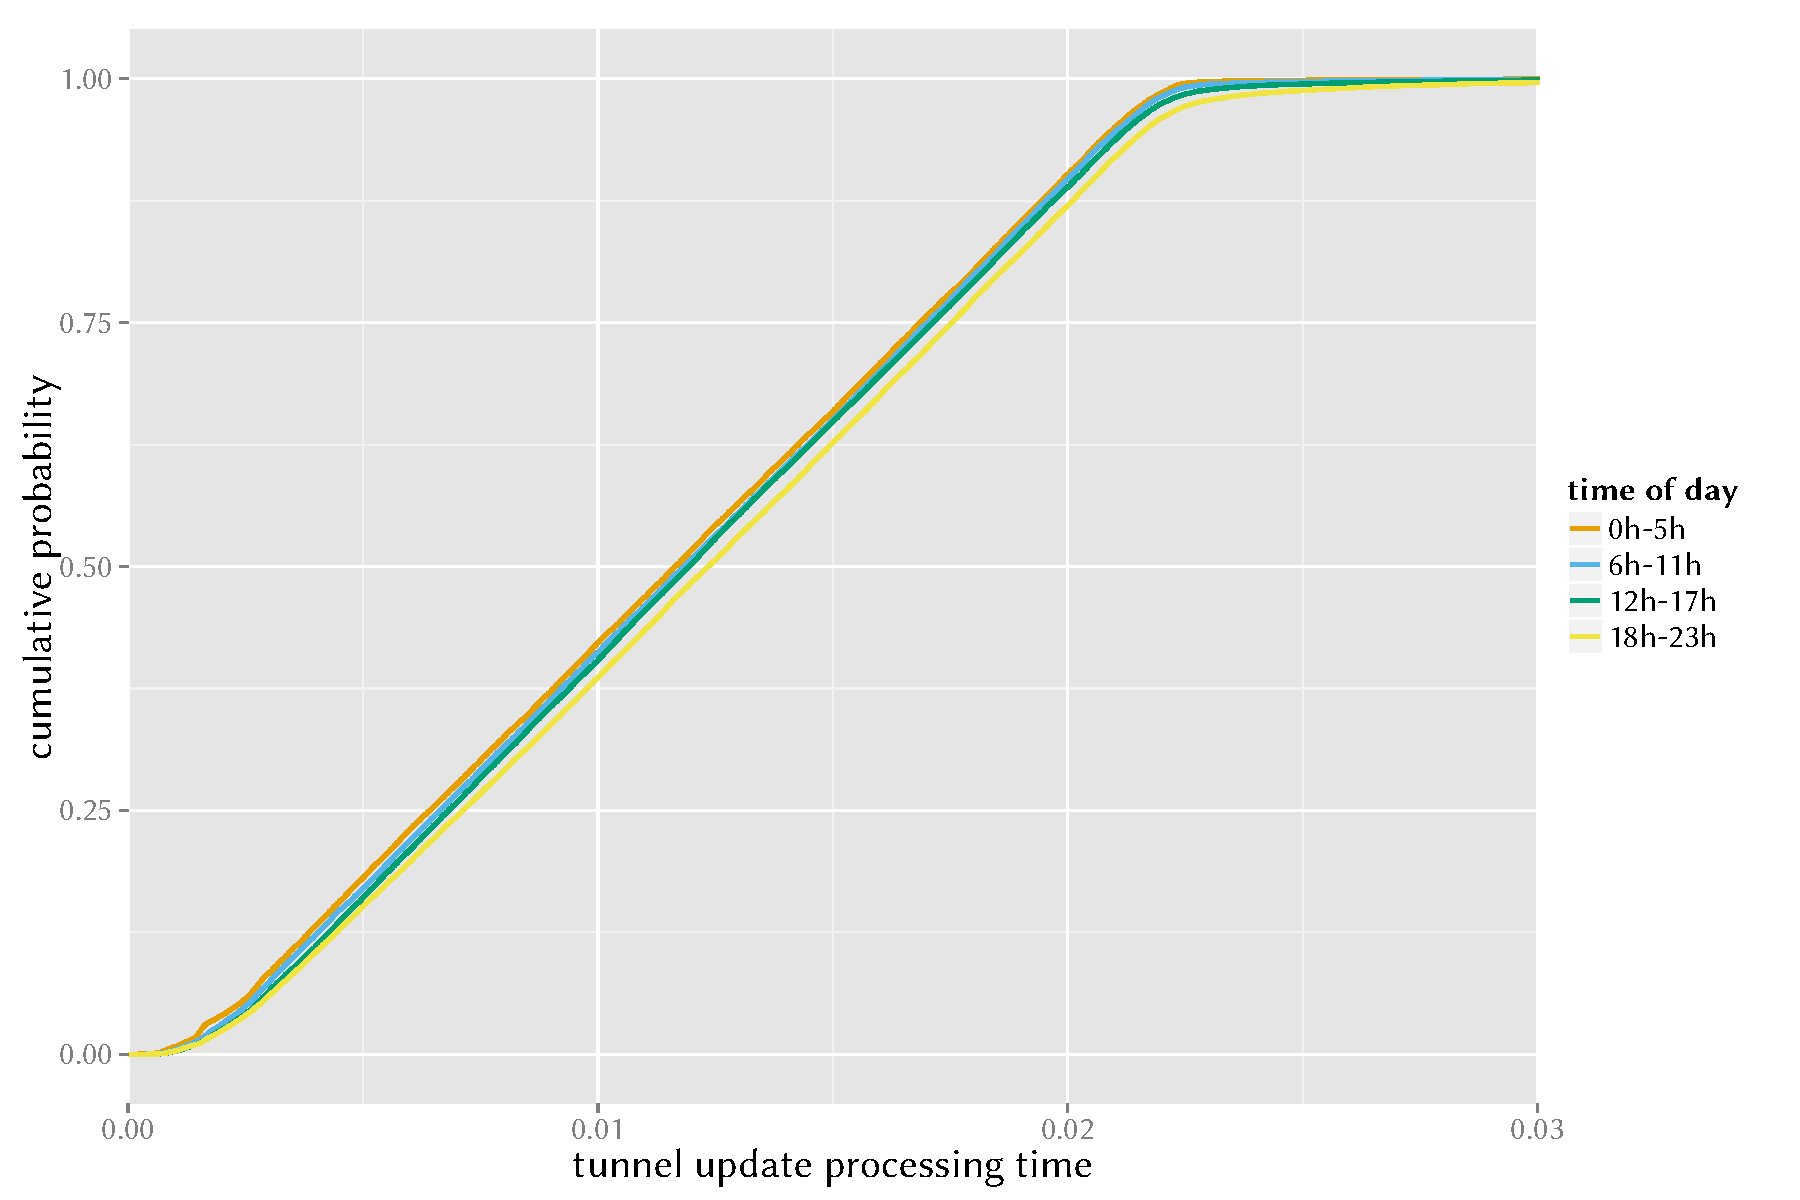
\includegraphics[width=0.9\textwidth]{images/R-update-time-cdfs.pdf}
	\caption{\acrshortpl{ECDF} of the time in seconds it takes a \acrshort{GGSN} to process a \acrshort{gtp} update event, separately plotted for four time slots each day.}
	\label{c4:fig:update-time}
\end{figure}

Figure~\ref{c4:fig:update-time} depicts a band of \glspl{ECDF} for the processing time of update messages by time of day. The processing time distribution almost perfectly follows a continuous uniform distribution between \SI{2}{\milli\second} and \SI{22}{\milli\second}. Only the upper end displays a slight long-tail behavior. The impact of the time of day is very slim with slightly higher processing times during the evening, the same time frame which also experienced an elevated arrival rate.

The occurrence of a continuous uniform distribution is rather unexpected as these do not usually occur in computing processes. According to the central limit theorem one would rather expect to see a normal distribution influenced by, e.g., process scheduling or other queuing artifacts. The source of this effect is still unknown and the current dataset does not allow for a more thorough investigation. Still, the fact that a higher update processing time coincides with an increase in the arrival rate points to an influence of tunnel messaging on the load of a \gls{GGSN}.



%%%%%%%%%%%%%%%%%%%%%%%%%%%%%%%%%%%%%%%%%%%%%%%%%%%%%%%%%%%%%%%%%%%%%%%%%%%%%%%
\subsection{Statistical Evaluation and Data Fitting}
\label{c4:sec:statistical_evaluation}

The uncovered empirical distributions for both the tunnel duration and the tunnel \gls{IAT} are now to be matched against theoretical probability distributions. Therefore, a univariate distribution fit to the experimental data was conducted. Having a concise representation for the empirical data will help in creating a model of the core network, which is the task conducted in the sections following after this.


%%
\paragraph{\gls{IAT} Fitting}

\begin{figure}[htb]
	\centering
	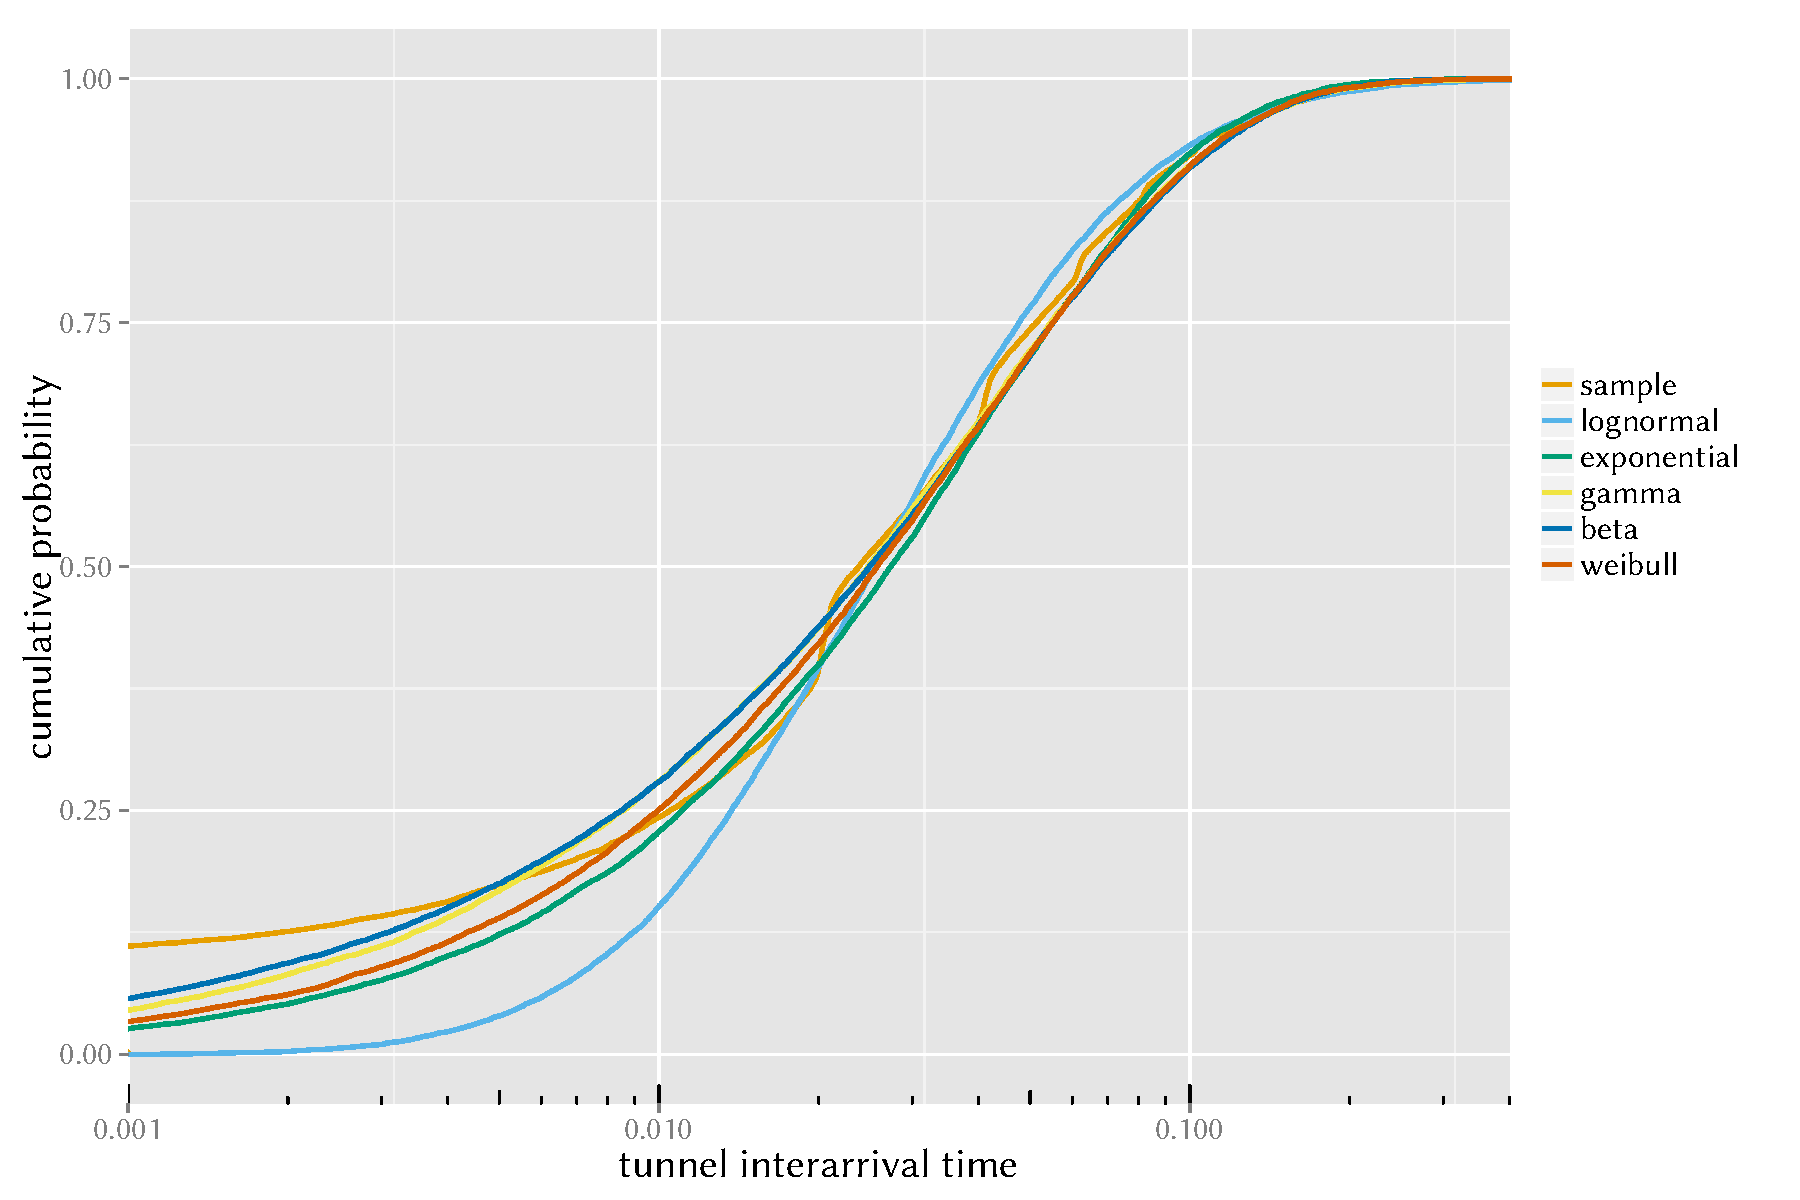
\includegraphics[width=0.9\textwidth]{images/R-IAT-ecdfs.pdf}
	\caption{Sampled inter-arrival time \acrshort{CDF} and fitted theoretical distributions.}
\label{c4:fig:IAT-cdfs}
\end{figure}

In order to investigate the tunnel \gls{IAT}, Figure~\ref{c4:fig:IAT-cdfs} displays the overall \gls{ECDF} with fits for various basic probability distributions. Each of the fits was generated through the method of moments matching.

The goodness of these fits was checked both visually using the \glspl{CDF} plots and numerically with goodness of fit measures, using Pearson's correlation coefficient and Pearson's $\chi^2$ test. Unfortunately, none of the probability distributions reaches the significance level for $\chi^2$. This can probably be largely attributed to the various previously described artifacts in the data. Matching them visually, the exponential fit seems to be reasonably close to the experimental data.

\begin{figure}[htb]
	\centering
	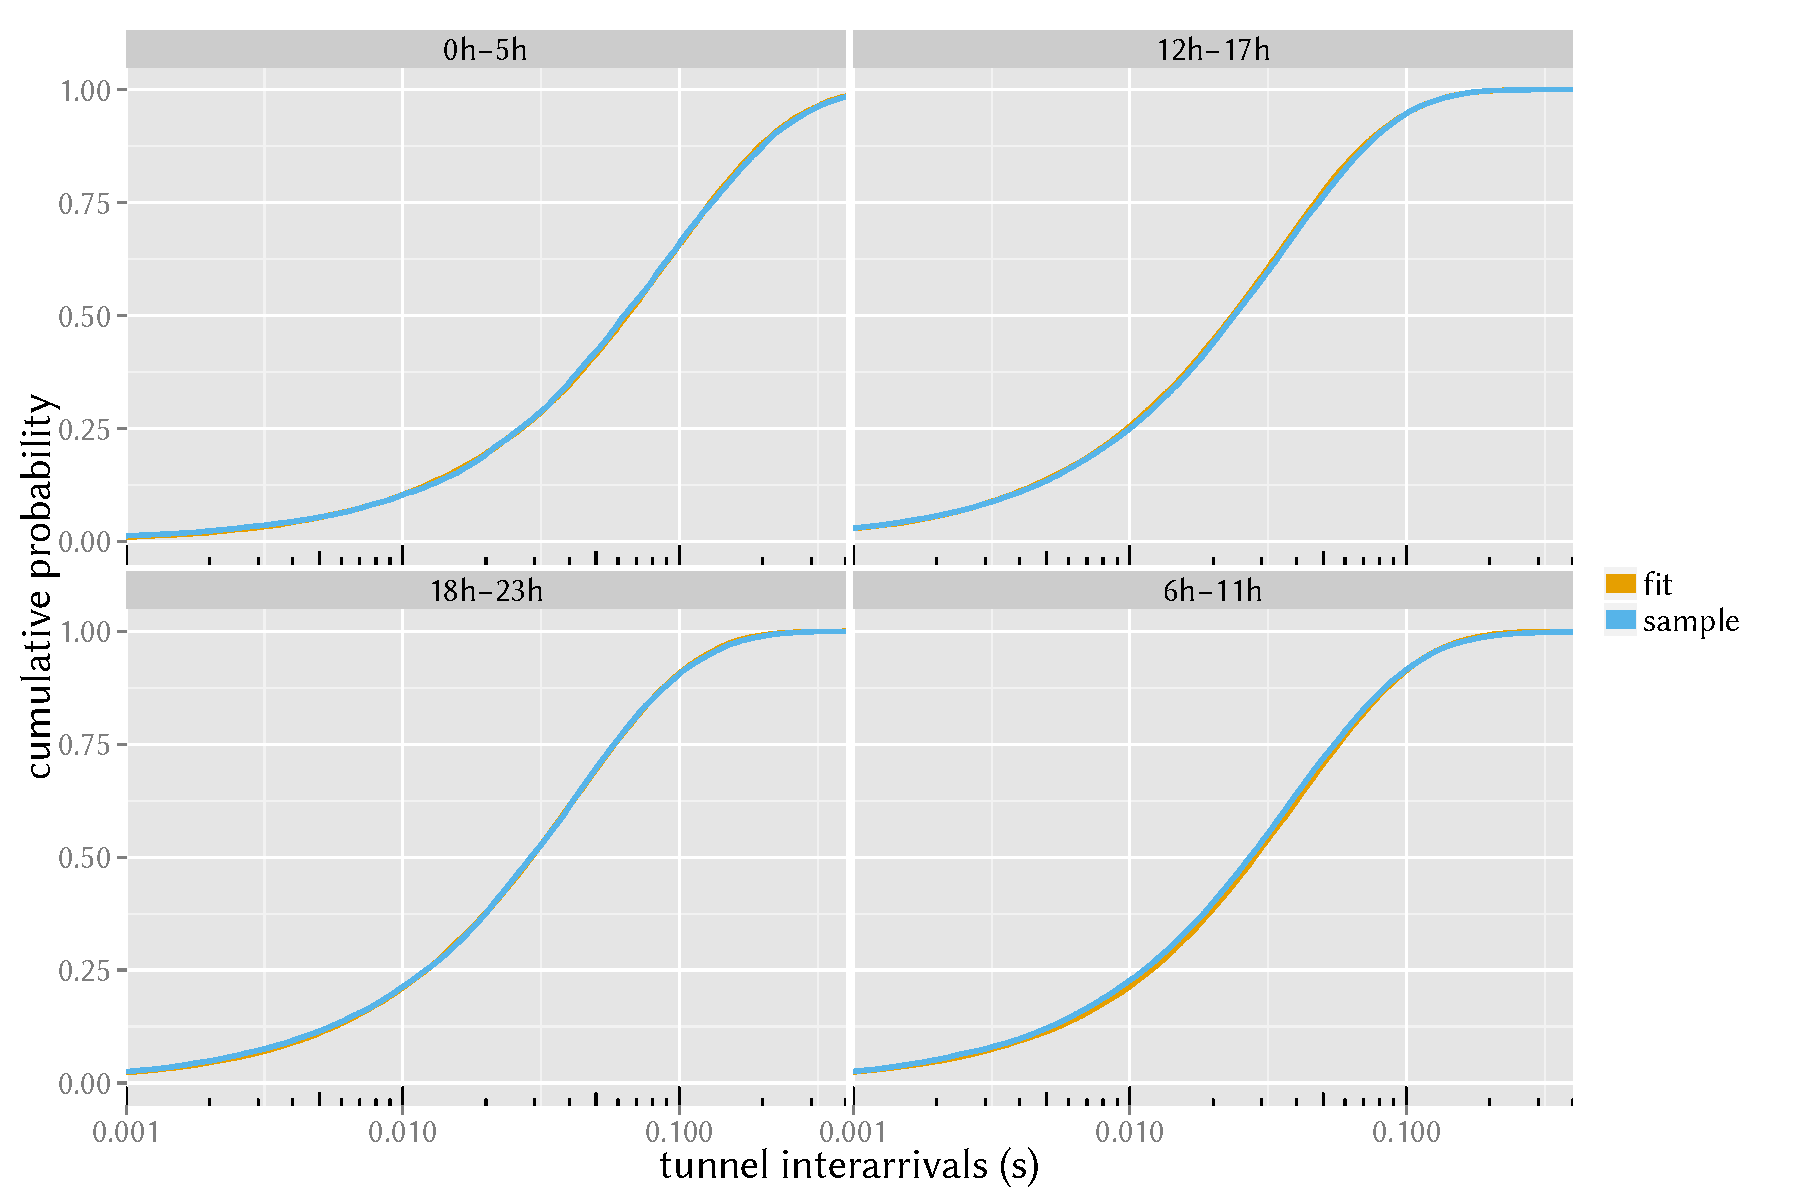
\includegraphics[width=0.9\textwidth]{images/R-IAT-active-fit-cdf-facets.pdf}
	\caption{Empirical and exponentially fitted \acrshortpl{CDF} of the tunnel \acrshort{IAT} by time of day. \acrshortpl{CDF} are overlapping as the coefficient of determination is close to $1$.}
\label{c4:fig:pdparrivalsecdf}
\end{figure}

To improve the fits, two modifications were made to the process. First, to remove the \SI{20}{\milli\second} steps, only the active tunnels were taken into consideration. Second, the overall \gls{IAT} distribution was once again split up into time of day slots. The overall distribution is just a superimposition of the individual slots anyway. Therefore, this should further improve the fidelity of the fits.

\begin{table}[htb]
\caption{Parameters for the exponentially distributed inter-arrival times and corresponding Pearson correlation coefficients.}
\label{c4:tab:IAT-fits}
	\centering
	\begin{tabu}{X[0.9,l]X[r]X[r]} 
	\toprule
	\textbf{Time of Day} & $\mathbf{\lambda}$ & $\mathbf{R_{arrival}}$\\ 
	\midrule
	0h-5h   & $10.67477$ & $0.995$ \\
	6h-11h  & $24.53298$ & $0.992$ \\
	12h-17h & $29.2504$  & $0.993$ \\
	18h-23h & $23.49983$ & $0.986$ \\
	\bottomrule
	\end{tabu}
\end{table}

The results are depicted in Figure~\ref{c4:fig:pdparrivalsecdf}. To improve plot visibility only four larger time slots are displayed here while the actual fits were conducted for each hour slot. Parameters for the exponential distribution $F(x) = 1- e^{-\lambda x}, x \geq 0$ and the corresponding correlation coefficients to the original data for the four time slots are given in Table~\ref{c4:tab:IAT-fits}. The fitted functions match the empirical data quite well, with some deviation present at the left tail but an overall positive correlation coefficient approaching $1$.


%%
\paragraph{Duration Fitting}

The second fitting effort surrounds the empirical data concerning the tunnel durations. However, none of the basic probability distributions (including exponential, gamma, and Weibull distributions) fit the tunnel duration even remotely. One of the reasons for this is probably that the tunnel duration is influenced by an overwhelming amount of factors, which were previously described. This superposition, especially with the user behavior, will result in unpredictable results that does not follow any basic probability distribution.

\begin{figure}[htb]
	\centering
	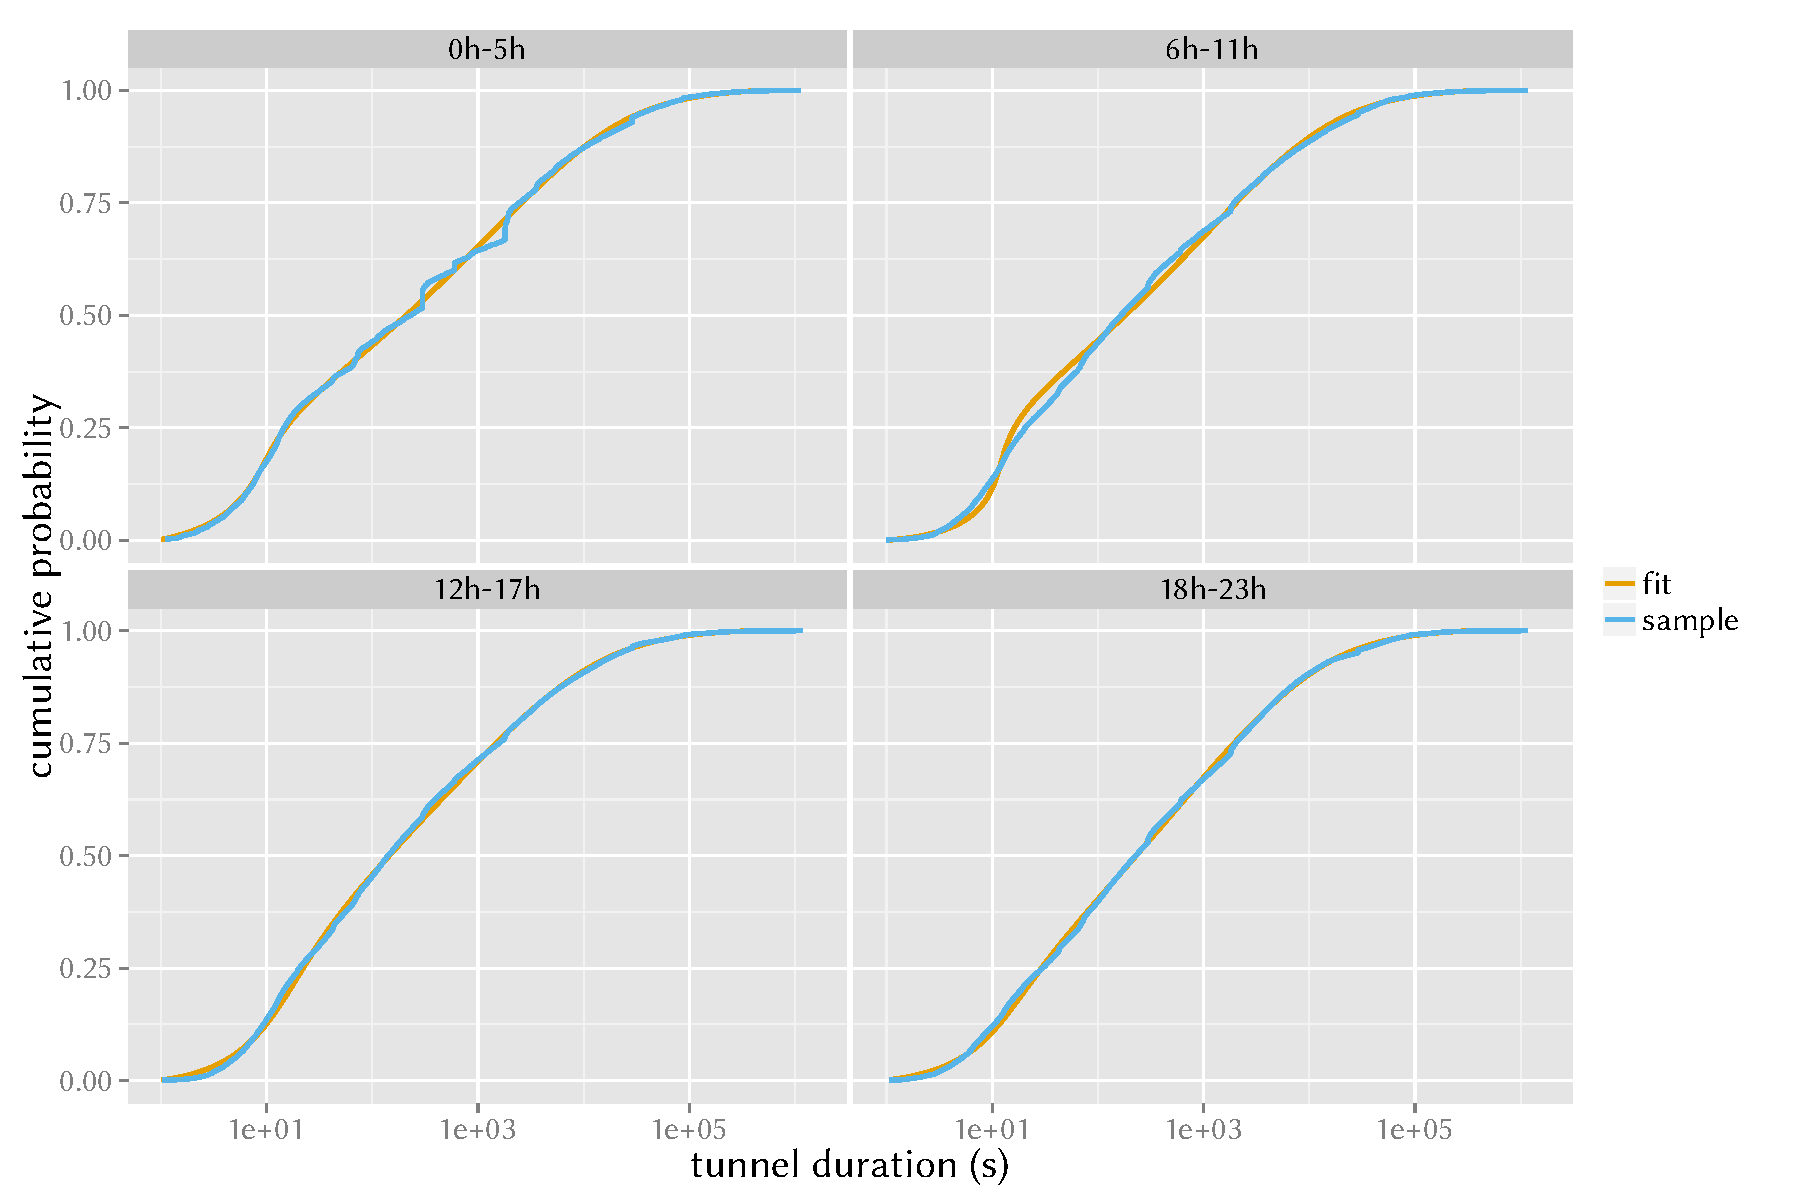
\includegraphics[width=0.9\textwidth]{images/R-duration-fit-cdf-facets.pdf}
	\caption{Empirical and fitted \acrshortpl{CDF} of the tunnel duration by time of day with fitted rational functions.}
\label{c4:fig:fittedsdurationlots}
\end{figure}

Instead, rational functions are fitted to the \glspl{ECDF} using the proprietary third-party tool \textit{Eureqa}~\cite{eureqa_paper, eureqa_software}. This allows for a much closer fit as seen in Figure~\ref{c4:fig:fittedsdurationlots}, but limits its application in the statistical evaluation.

\begin{table}[htb]
\caption{Inverse rational functions fitted to the \acrshortpl{ECDF} of the tunnel duration by time of day and correlation coefficients of the fit.}
\label{c4:tab:fits-duration}
	\centering
	\begin{tabu}{X[1.1,l]X[4.5,r]X[r]} 
	\toprule
	\textbf{Time of Day} & \textbf{Inverse Serving Time \gls{CDF} Representation} & $\mathbf{R_{dur}}$\\ 
	\midrule
	0h-5h & $0.919 - 60.614y - 3498.78y^3 - \frac{110.707y + 2289.94y^3}{y - 1.005}$ &  $0.999$ \\
	6h-11h & $1 + 117.484y - 368.643y^2 - \frac{1720.13y^4}{y - 1.004}$ & $0.999$ \\
	12h-17h & $0.953 + 69.491y + \frac{81146.1y^3 + 1.086\times10^6y^5}{805 - 802.01y}$ & $0.999$ \\
	18h-23h & $0.912 + 82.056y - \frac{2936.93y^4}{1.945y - 1.953}$ & $0.999$ \\
	\bottomrule
	\end{tabu}
\end{table}

	% high precision:
	% 0h-5h & $0.919208 - 60.6136y - 3498.78y^3 - \frac{110.707y + 2289.94y^3}{y - 1.00469}$ &  $0.999$ \\
	% 6h-11h & $1 + 117.484y - 368.643y^2 - \frac{1720.13y^4}{y - 1.0041}$ & $0.999$ \\
	% 12h-17h & $0.952566 + 69.4907y + \frac{81146.1y^3 + 1.08572\times10^6y^5}{805 - 802.01y}$ & $0.999$ \\
	% 18h-23h & $0.911924 + 82.0562y - \frac{2936.93y^4}{1.94468y - 1.9532}$ & $0.999$ \\

Table~\ref{c4:tab:fits-duration} contains the functions which were fitted to the \textit{inverse} \gls{CDF}. The inverse was chosen here to simplify the modeling and simulation process coming afterwards. The functions can be easily inverted again for other purposes. Both the \glspl{CDF} in the plot as well as the Pearson correlation coefficient, which again approach $1$, confirm the goodness of the fitted functions.


% \begin{table}
% \centering
% \caption{TAC Statistics}
% \begin{tabu}{|X|X|X[1.5]|X|X|X|} \hline
% & \textbf{\# of Flows} & \textbf{Total Traffic (Bytes)} &  \textbf{\# of Tunnels} & \textbf{\# of GTP Signalling Msgs} & \textbf{\# of Distinct IMSIs}\\ \hline
% Total          & 2234659247 & 122758578593993 (112TB)    & 16632094 & 409733865 & 1255293 (all) / 1030895 (with flows) \\ \hline
% In TAC DB      & 2228315260 & 122716712007150 (111.61TB) & 14565430 & 372662108 & 1015891 \\ \hline
% Smartphones    & 459990512  & 15721818747754 (14.30TB)   & 10030734 & 311342846 & 476675  \\ \hline
% Regular phones & 5705832    & 448140315058 (0.41TB)      & 897529   & 3860162   & 116124  \\ \hline
% 3G dongles     & 1487230062 & 92215931895630 (83.87TB)   & 2114756  & 39053819  & 315003  \\ \hline
% Android        & 241973565  & 7953178401958 (7.2TB)      & 2383255  & 177537567 & 175919  \\ \hline
% iOS            & 161408903  & 5481693567152 (5TB)        & 3145384  & 83374590  & 99679   \\ \hline
% Symbian        & 22827418   & 1332996529271 (1.21TB)     & 3520242  & 18479002  & 162790  \\ \hline
% Blackberry OS  &            & 128074907884 (0.12TB)      &          &           &         \\ \hline
% \end{tabu}
% \end{table}


%Devices with GTP signaling but no user plane traffic: (\#distinct imsis gtp db)-(\#distinct imsis flow db):
% $255293-1030895=224398\text{ or }17.88\%$

%%%%%%%%%%%%%%%%%%%%%%%%%%%%%%%%%%%%%%%%%%%%%%%%%%%%%%%%%%%%%%%%%%%%%%%%%%%%%%%%
%\subsection{Correlations to User Traffic}
% TODO, incl. measurements



%%%
% Direct signaling traffic overhead in relation to user traffic and induced network load

% GTP Header: 12 Byte
% IE header and footer: 2 Byte
% Maximum minimum data size including all \glspl{IE}: 221 Byte + 12 Byte Header + 2*37 Extension Header = 307 Byte
% Minimum size of message with just mandatory \glspl{IE}: 12 + 30 + 2*5 = 52 Byte

% 307 Bytes:
% calculation from our dataset
% Total maximum signaling traffic with this calculation: 117.15GB
% Ratio: 0.10\%
% 52 Bytes:
% Total maximum signaling traffic with this calculation: 19.84GB
% Ratio: 0.02\%
% Total traffic: 122758578593993


% signaling calc:
% gtp signaling traffic volume estimation $v_s$ = (1059B gtp message + 8B udp header + 20B ipv4 header) = 1087B * 409733865 number of request/response pairs * 2 (2 messages per pair) = 8,9076142E11B
% ratio to total $r=\frac{v_s}{v_t}=0.72\%$  $v_t=122758578593993B$


%%
%TODO: radio access type plots, if we have the data
% We do not.
%
%\begin{figure}
%\centering
%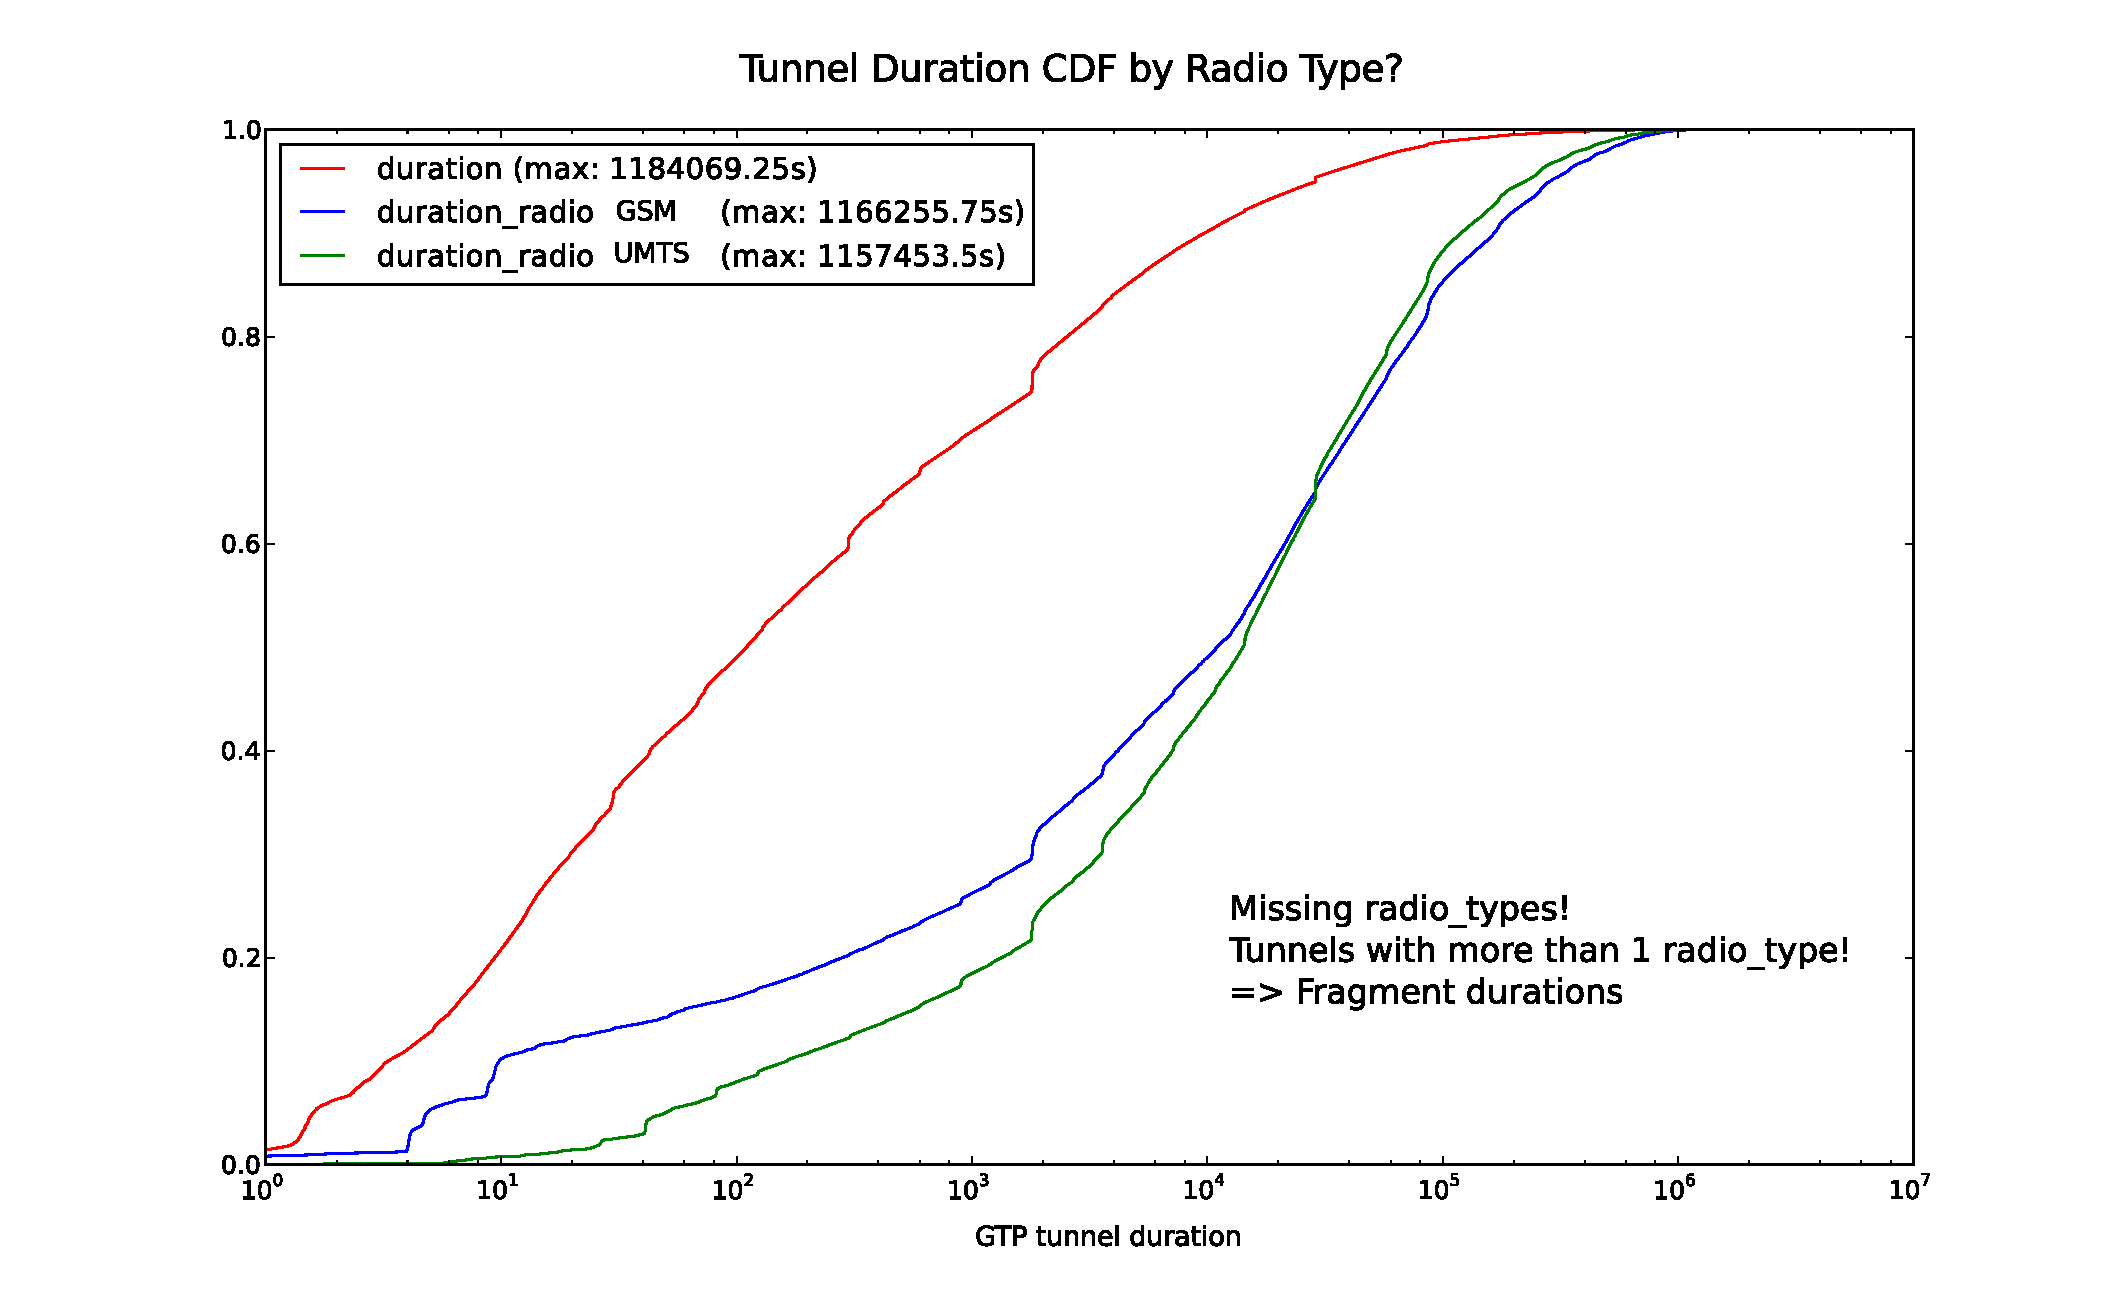
\includegraphics[width=\columnwidth]{figures/tunnel-dur-radio-cdf-mod.pdf}
%\caption{Tunnel duration distribution, separated for UMTS and GPRS radio access [NOTE: only in the last tunnel segment; and majority of radio types %is unknown anyway.}
%\label{fig:cdf-duration-radio}
%\end{figure}


%%%%%%%%%%%%%%%%%%%%%%%%%%%%%%%%%%%%%%%%%%%%%%%%%%%%%%%%%%%%%%%%%%%%%%%%%%%%%%%%
%!TEX root = ../../dissertation.tex
%%%%%%%%%%%%%%%%%%%%%%%%%%%%%%%%%%%%%%%%%%%%%%%%%%%%%%%%%%%%%%%%%%%%%%%%%%%%%%%%
\section{Streaming Modeling}
\label{c3:sec:modeling}

As stated, the goal of this chapter is to model the measuring process and reliable streaming. This section will introduce our reliable \gls{TCP}-based streaming model. It is intended for easily comparing different protocol variants against each other and measuring all variants in one testbed. 

But first, because any evaluation of a model requires metrics, we describe ones appropriate to the model and give a rationale.
 
%%%%%%%%%%%%%%%%%%%%%%%%%%%%%%%%%%%%%%%%%%%%%%%%%%%%%%%%%%%%%%%%%%%%%%%%%%%%%%%%
\subsection{Metrics for Reliable Transport Streaming}
\label{c3:metrics}

When measuring anything related to video or even just image quality, one has the choice between conducting a subjective or objective assessment. 

During a subjective test, human assessors evaluate and rate video quality in a controlled environment with the results usually being aggregated into an overall relative quality score \gls{MOS}. Through the human element, conducting a subjective assessment is very time and resource consuming but it also achieves the highest precision.

This is where, objective video quality assessments come into play. Modern objective models attempt to recreate the features of the humans' visual perception and psychophysics and are calibrated by subjective assessments. Most objective models operate on a full reference approach, they directly compare the original reference video to the resulting video after being encoding or transmitted.

Two of the simplest full reference image quality metrics, which can also be applied on video, are the \gls{MSE} and \gls{PSNR}, defined as:

\begin{equation}
    \begin{aligned}
    MSE = \frac{1}{N} \sum_{i=1}^{N}(x_i - y_i)^2\\
    \text{and } PSNR = 10 \log_{10} \frac{L^2}{MSE},
    \end{aligned}
\end{equation}

with $N$ as the number of pixels in a frame and individual pixels $x$ and $y$ from the reference and output frame respectively. $L$ denotes the maximum value of a pixel. For grayscale or when investigating each color channel separately, usually $L = \SI{8}{\bit} = 255$.  \cite{objective-vqa}

Image quality models can by nature only test for spatial distortions of a single image. This includes a general blockiness or blurriness, noise, or reduced resolution. Dedicated video quality assessments can additionally take temporal metrics into account, e.g. frame rate anomalies. Such models are being researched and standardized by the \gls{ITU} and \gls{VQEG} for example in \cite{ituJ144, ituJ246, ituJ247}.


When conducting dedicated streaming quality measurements, only this portion should be taken into account by a metric, and not the initial encoding process. During streaming only a specific subset of quality degradations can occur. Lost or late packets can cause missing blocks in a frame or frames to be skipped completely. Initial thoughts concerning \gls{IPTV} \gls{QoE} have been given in \cite{ituG1080} and the influence of packet delay variations on playout buffers is investigated in \cite{rfc3393}The \gls{MDI} \cite{rfc4445} is an attempt to capture this behavior and relate it to the network \gls{QoS}. Its metric relies on two properties, the \gls{DF}, as a measure of the network's latency and jitter, and the media loss rate. Of special interest to this investigation is the \gls{DF}, which is calculated based on a virtual buffer (VB) of received stream data as

\begin{equation}
    \begin{aligned}
        VB = r_{rcv} - r_{drain} \\
        DF_i = \frac{\max(VB) - \min(VB)}{r_{drain}}
    \end{aligned}
\end{equation}
 
Reliable streaming has even less possibilities to degrade a video stream. Packets can not be out of order and loss is concealed by \gls{TCP}, meaning that the transmitted and the played video are identical. The only thing that can still happen, is portions of the video arriving too late to be played out at their intended point in time.
A potential reliable streaming quality assessment metric needs to keep track of the following properties:

\begin{itemize}
    \item The initial delay, which is the time delta between the start of the transmission and the start of the video play.
    \item The number and lengths of interruptions or stalls during playback.
    \item For adaptive streaming, the characteristics of the quality levels the video was played in. This includes the number of switching events and the duration of each level.
\end{itemize}

A concise metric covering all properties has not been defined yet. The \gls{CI} was defined in \cite{1498486} and used to determine quality in \gls{P2P} live streaming. It is defined as \enquote{the number of segments that arrive before or on playback deadlines over the total number of segments} and with this partly captures the stalling property. In \cite{5634160} and \cite{DBLP:journals/corr/SeyedebrahimiBP13} a so-called \gls{PI} is defined and evaluated. The definition $I_p = uv$ is simply based on the number of stalls $u$ and the average stall duration $v$. 

Generally, most research operates just directly on these three properties, which allows for the most freedom in usage scenarios. The streaming measurement model presented in the following section also works with the assumption, that only the three properties are of importance. The model assumes no special metric, the individual properties can be directly attained from the model. Though any metric could still be applied on the results.


%%%%%%%%%%%%%%%%%%%%%%%%%%%%%%%%%%%%%%%%%%%%%%%%%%%%%%%%%%%%%%%%%%%%%%%%%%%%%%%%
\subsection{Measurement and Playback Model}
\label{c3:model}

Parts of the model presentation is based on the author's previous work published in \cite{cs3518}, \cite{metzger2011delivery}, and \cite{6229739}. It is based on the desire to compare all in-the-wild variants of reliable streaming protocols in a simple and concise way. This is achieved by basing the model on the component that is common to all of the approaches: the playback buffer.

To display a video stream, an application needs to maintain a playback buffer of sufficient size to at least gather enough data to reconstruct one single atomic unit of playback such as a video frame.
From the perspective of a player application , a video consists of a sequence of atomic units, video frames and audio samples.
The application progressively decodes the video from a source and stores the units temporarily in a memory buffer before playing them. In reliable streaming, the buffer is filled by the payload from received \gls{TCP} segments a subject to the network \gls{QoS}. The process can be subsumed as:

\begin{equation*}
\mathit{buffer}(t) = \sum_{0}^{t} \text{data}_\mathrm{received} - \sum_{0}^{t} \text{data}_\mathrm{played}
\end{equation*}

Both the incoming and outgoing data stream are variable over time. The fill level of the playback buffer is the critical component in the playback process and the central element of the model.If the buffer reaches a size of zero the playback process stops and stalling occurs.

\begin{figure}[htb]
    \centering
    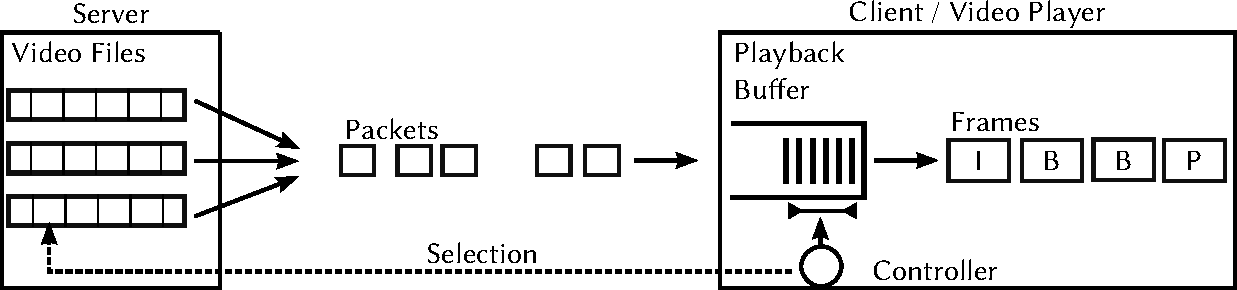
\includegraphics[width=0.9\textwidth]{images/playback-model.pdf}
    \caption{Reliable streaming playback model based on buffer control.}
    \label{c3:fig:playback-model}
\end{figure}

Figure~\ref{c3:fig:playback-model} overviews the reliable streaming model. The controller, part of the video player, selects a video from a remote location and the transmission is started, filling the playback buffer. The model has three degrees of freedom, which are all governed by the controller and together are coined playback strategies. These are:

\begin{itemize}
    \item The initial playback delay, which is the time between the initiation of the video stream transmission and the actual stream playback. The larger this is chosen, the bigger the safety margin on the buffer gets. If the video and transmission bitrate are known to be constant and and appropriately dimensioned, the initial delay can be chosen to be very small.
    \item Playback pause and resume decisions based on the current buffer fill level. This is a generalization of the initial playback delay, which is in fact only one, albeit always occurring stalling period.
    \item Selection of the video or video segment with a video bitrate chosen according to the current network throughput. This is only applicable for adaptive streaming.
\end{itemize}


These decisions yield a stalling period distribution for a streamed video. The frequency and the duration of stalls directly relate to the decision function of the playback model. The more frequent the stalls are, the shorter they will be; if the strategy produces longer stalls, they will be less frequent assuming the same network conditions. The time scale on which streaming applications buffer content usually lies in the range of seconds. This is a necessity in best-effort networks, as the available network bitrate might drop unexpectedly and cause stalling.


The the rest of this sections present fundamental playback strategies and strategy building blocks with features extracted from real world examples, which are given afterwards. 



%%
\subsubsection{Null Strategy}

The simplest strategy is having no strategy at all. Playback is started immediately when at least a single frame fully resides within the buffer and stops again at an empty buffer. The behavior can be summarized as ``Whenever anything can be played from the buffer, do so''.

This results in frequent stops and a large loss in playback continuity and will therefore not be used in practice. However, this strategy has some interesting theoretical properties, which is why it is mentioned here.
It minimizes total stalling time and the required buffer space. Moreover, it gives an upper limit for the number of stalls occurring\footnote{As a video frame is atomic, no other model could possibly stop the playback more often.}. Therefore, it can act as a baseline reference to assess the performance of other strategies.

\begin{figure}[htb]
    \centering
    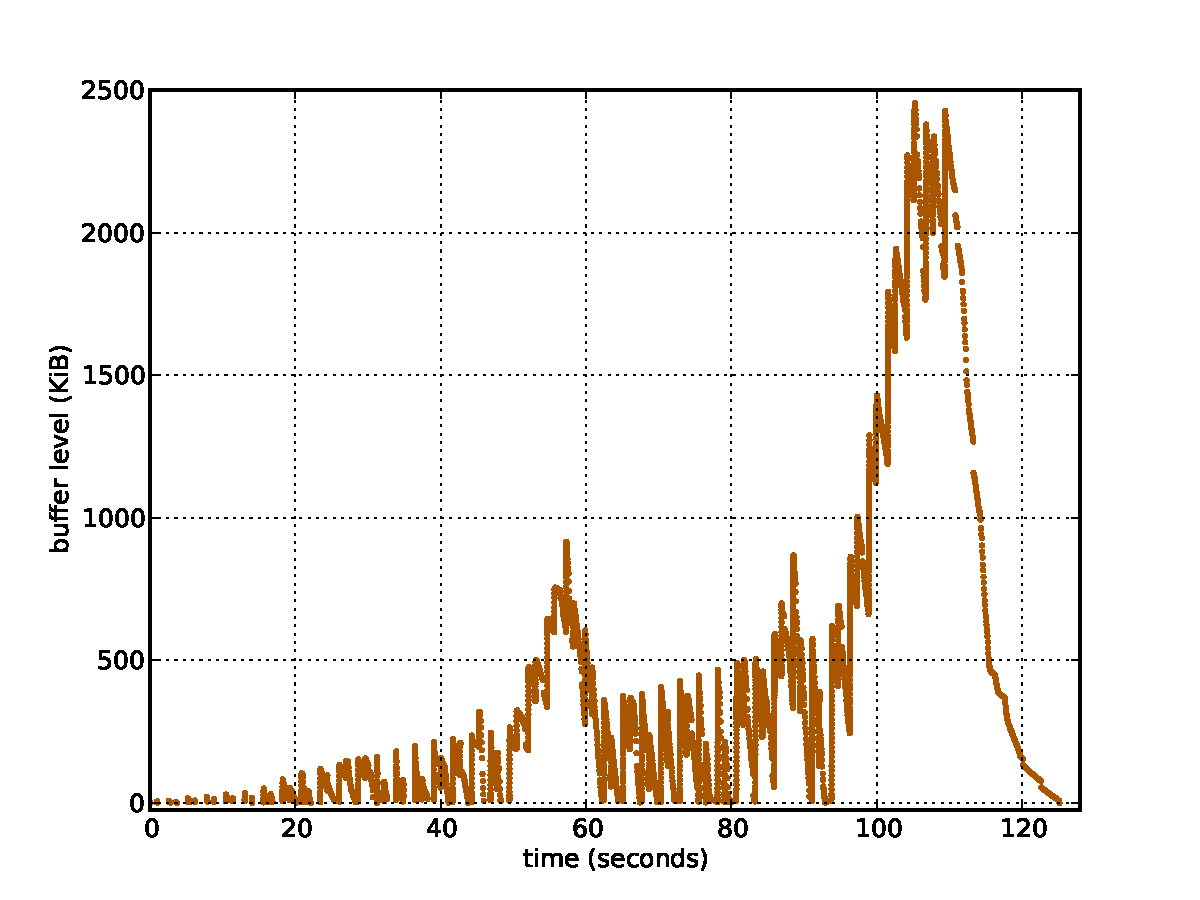
\includegraphics[width=0.9\textwidth]{images/bufferlevel-stall-new.pdf}
    \caption{Buffer fill level with null strategy; \SI{33}{\second} total stalling.}
    \label{c3:fig:bufferlevel-stall}
\end{figure}

Figure~\ref{c3:fig:bufferlevel-stall} depicts an exemplary time series diagram of the contents of a video buffer using this strategy with a transmission rate only slightly above the video stream's rate. The buffer frequently drops down to zero forcing a short stall. According to the presented related work on the \gls{QoE} impact of stalling frequency in comparison to the length of stalls \cite{6123395}, this is the worst possible scenario for a person watching the stream.


%%
\subsubsection{Threshold Strategies}

Instead of instantly restarting playback, a lower threshold can be introduced. Only after a certain buffer fill level threshold has been surpassed, playback will be started. Thresholds can be set independently for the initial playback delay and stalls, with the initial playback delay generally set to be higher.

The threshold can be chosen in a number of ways. It can either be an absolute data volume, a buffered video duration. The latter is much more suited for variable bitrate videos as it automatically adapts itself to the current bitrate. A third option is to buffer for a certain amount of real time -- this can be seen as threshold -- and starting playback after that period regardless of the volume of the buffer. Additionally, the threshold could also either be set to a constant value or dynamically chosen according to the expected network \gls{QoS}.

Besides this single-threshold strategy, a two-threshold strategy might make more sense for segment-based streaming. In addition to the lower threshold, an upper threshold is introduced. When reached, no new segments will be requested until the buffer arrives at the lower threshold again.  To achieve an hysteresis effect a third threshold, somewhere between the lower and upper bound, can also be introduced. Through this, the maximum buffer size can also be controlled. This is important in situations with hard limits on available memory. Mobile devices come to mind here.

\begin{figure}[htb]
    \centering
    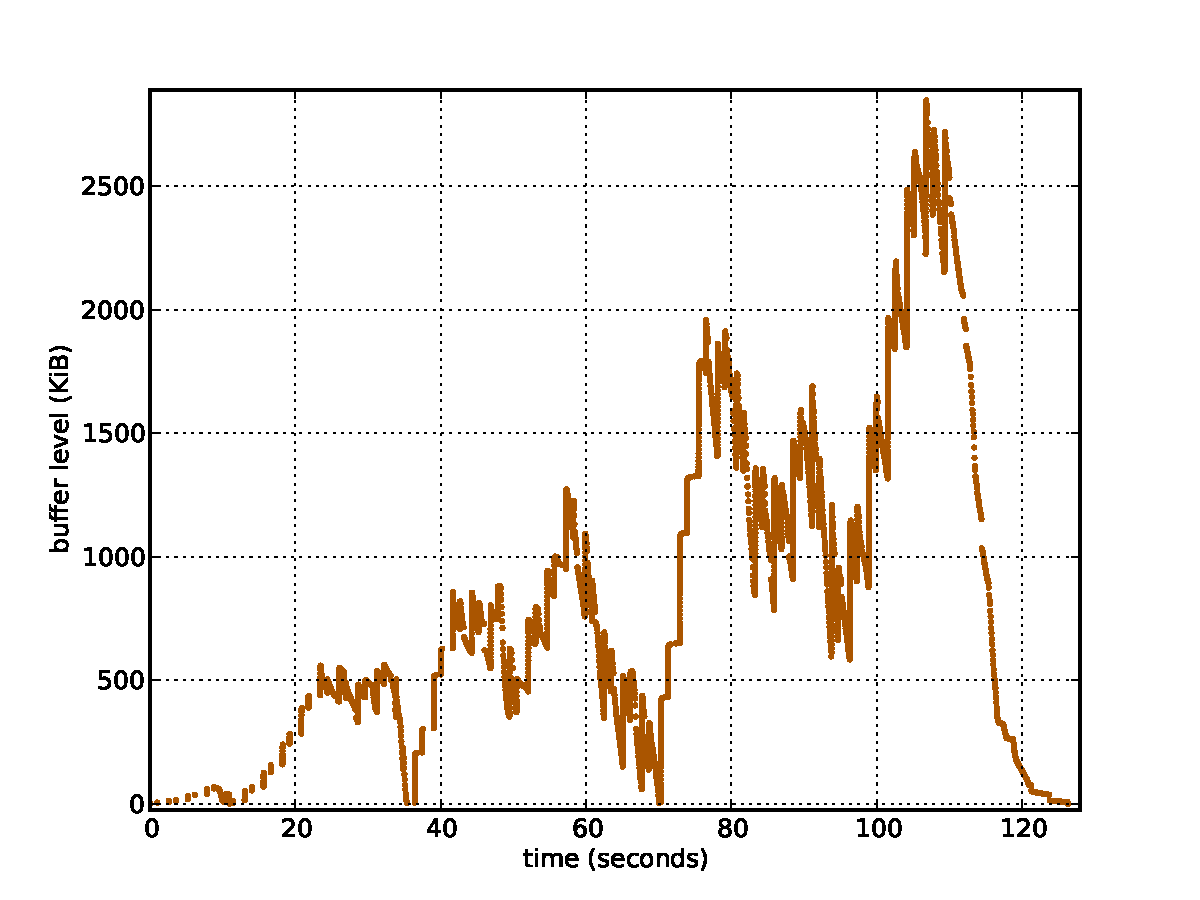
\includegraphics[width=0.9\textwidth]{images/bufferlevel-flash-new.pdf}
    \caption{Sample buffer fill level for a \SI{2}{\second} and \SI{5}{\second} buffered video duration threshold strategy; \SI{34}{\second} total stalling.}
    \label{c3:fig:bufferlevel-flash}
\end{figure}

An example buffer diagram is displayed in Figure~\ref{c3:fig:bufferlevel-flash}. In this case, the initial delay was controlled by a buffered video duration threshold of \SI{2}{\second} and a resume condition also based on buffered video duration but with a \SI{5}{\second} threshold. The strategy produces noticeable less stalls than the null strategy but slightly increases the total stalling time.


%%
\subsubsection{Pacing Strategies}

For segment-based \gls{HTTP} streaming, a two-threshold strategy is not the only supplemental option on top of simple streaming. Here, the controller can pace the request of future segments to match the overall, or the current video bitrate. A safety margin can also be factored in to even out short time fluctuations of either the transmission or the video bitrate. For example, the controller would request segments with an overall transmission rate of 1.25 times the video bitrate. The pacing rate can either be statically chosen in advance or can be calculated dynamically based on current or future conditions. The latter leads to predictive strategies.

%%
\subsubsection{Predictive Strategies}

In predictive strategies, knowledge of the future of the streaming process is used by the controller to adjust the start/stop and segment retrieval conditions. Instead of global knowledge, heuristics can instead attempt to approximate a future state.

A very simple predictive approach is to prolong the initial delay to the point, that no intermediate buffer underrun and thus no stall will occur. With global knowledge, the controller can start the stream at the earliest possible point in time, thus minimizing the total stalling time while still having only the initial delay.

\begin{figure}[htb]
    \centering
    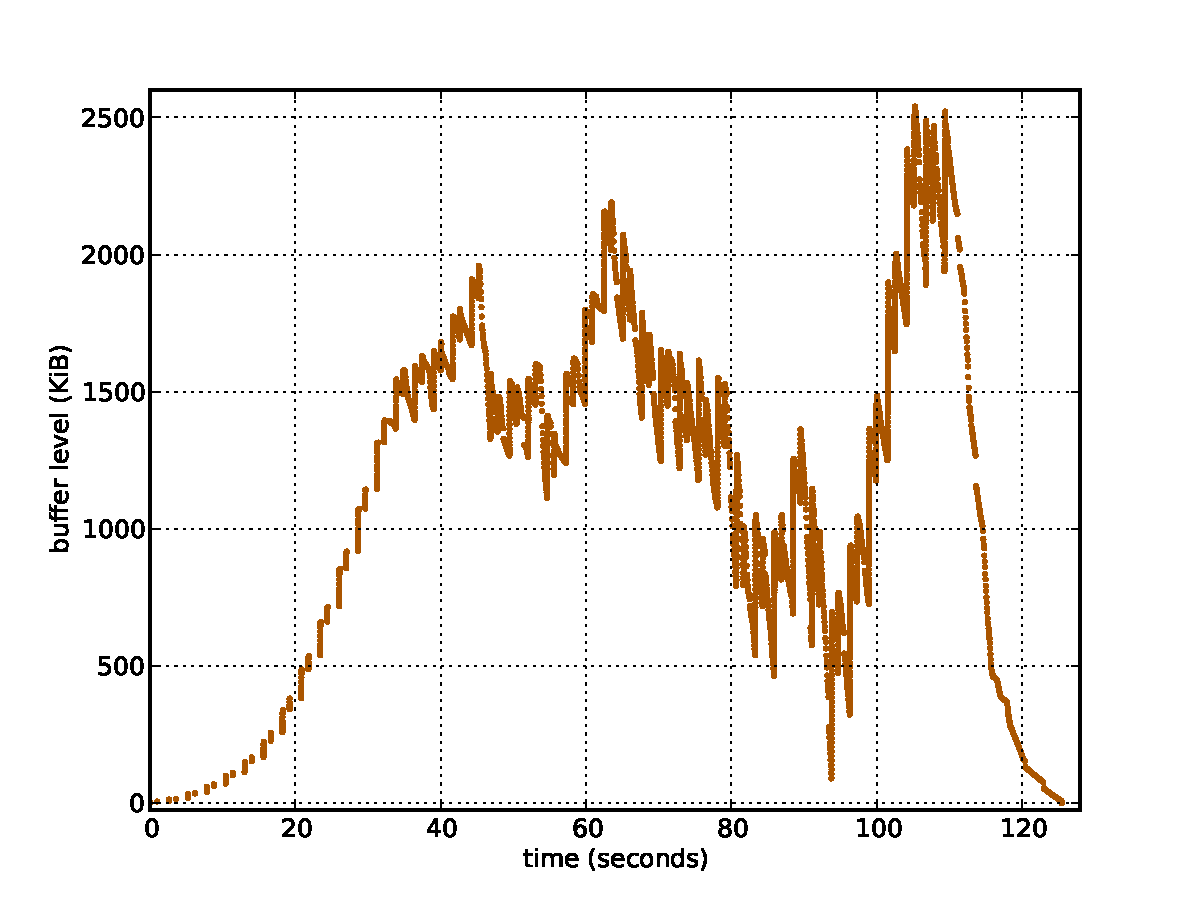
\includegraphics[width=0.9\textwidth]{images/bufferlevel-startdelay-new.pdf}
    \caption{Sample Buffer fill level for the delayed playback model, \SI{33}{\second} total stalling.}
    \label{c3:fig:bufferlevel-startdelay}
\end{figure}

Figure~\ref{c3:fig:bufferlevel-startdelay} depicts the time series of a sample implementation of this delayed playback predictive strategy with all necessary stalling occurring upfront.


%%
\subsubsection{Adaptive Strategies}

Most strategies for adaptive streaming are an extension of both the threshold as well as the pacing strategy. However, instead of a simple transmit-or-no-transmit ruleset, they can make much more fine-grained adjustments. The quality of the stream segment to be requested will be chosen, depending on the current fill level and drain rate of the buffer. This makes a trade off between maintaining a certain quality level and putting up with increased waiting times, and dropping the quality to a level sustainable at the current transmission rate.


\subsubsection{Real World Implementation Examples}

Actual streaming player implementations often do not implement only one of these strategies, but rather combine ideas from several. Herein, thresholds are often set arbitrarily through the implementor's best practices and not empirically evaluated, often making a trade-off between user perceivable quality and resulting server load. In general, every streaming service practically implements its own playback strategies. This section describes three example applications.

%%
\paragraph{2011 YouTube Flash Player Buffering Strategy}

Google's video streaming site YouTube is constantly changing its appearance and technical makeup. In recent years, YouTube streams are delivered by one of three players: The Website's Flash player, a browser-integrated HTML5-based player, or custom player implementations in mobile phones, set-top boxes and similar devices. Here, the Flash-based variant used in 2011 is described.

This player used a single threshold strategy with different threshold values for the initial delay and any subsequent stalls. The values were already described in Figure~\ref{c3:fig:bufferlevel-flash}. This model assumes sufficient network conditions in the beginning, requiring only a short initial playback delay to pre-fill the playback buffer. If, however, stalling occurs, then it will buffer longer to keep the stalling frequency down.

\begin{table}[htb]
    % increase table row spacing, adjust to taste
    %\renewcommand{\arraystretch}{1.3}
    \caption{Transmission Related Parameters from YouTube's Video URL Setup}
    \label{c3:tbl:yturl}
    \centering
    \begin{tabu}{|X[l]|X[p]|}
        \hline
        URL Part & Description \\ \hline
        \texttt{v$\alpha$.lscache$\beta$.c.youtube.com} &  Cache server involved in the delivery.\\
        \texttt{algorithm=throttle-factor} and \texttt{burst=40} and \texttt{factor=1.25} & Indicates initial burst plus block sending configuration. \\
        \texttt{ratebypass=yes} & Parameter to indicate no rate limiting.\\ \hline
    \end{tabu}
\end{table}

Furthermore, YouTube employs a proprietary pacing mechanism outside of the control of the streaming player. This is hinted at in the encoding of the \glspl{URL} of the video files and enforced by the video file cache server. Some of those not user-changeable parameters are described in Table~\ref{c3:tbl:yturl}. The pacing was in effect for all videos below high definition resolution, but has since then been extended to include all video files. 

\begin{figure}[htbp]
% used yt-delay/hPUGNCIozp0_delay_100 2, spyder with matplotlib config patch
    \centering
        \begin{subfigure}[b]{0.90\textwidth}
                \centering
                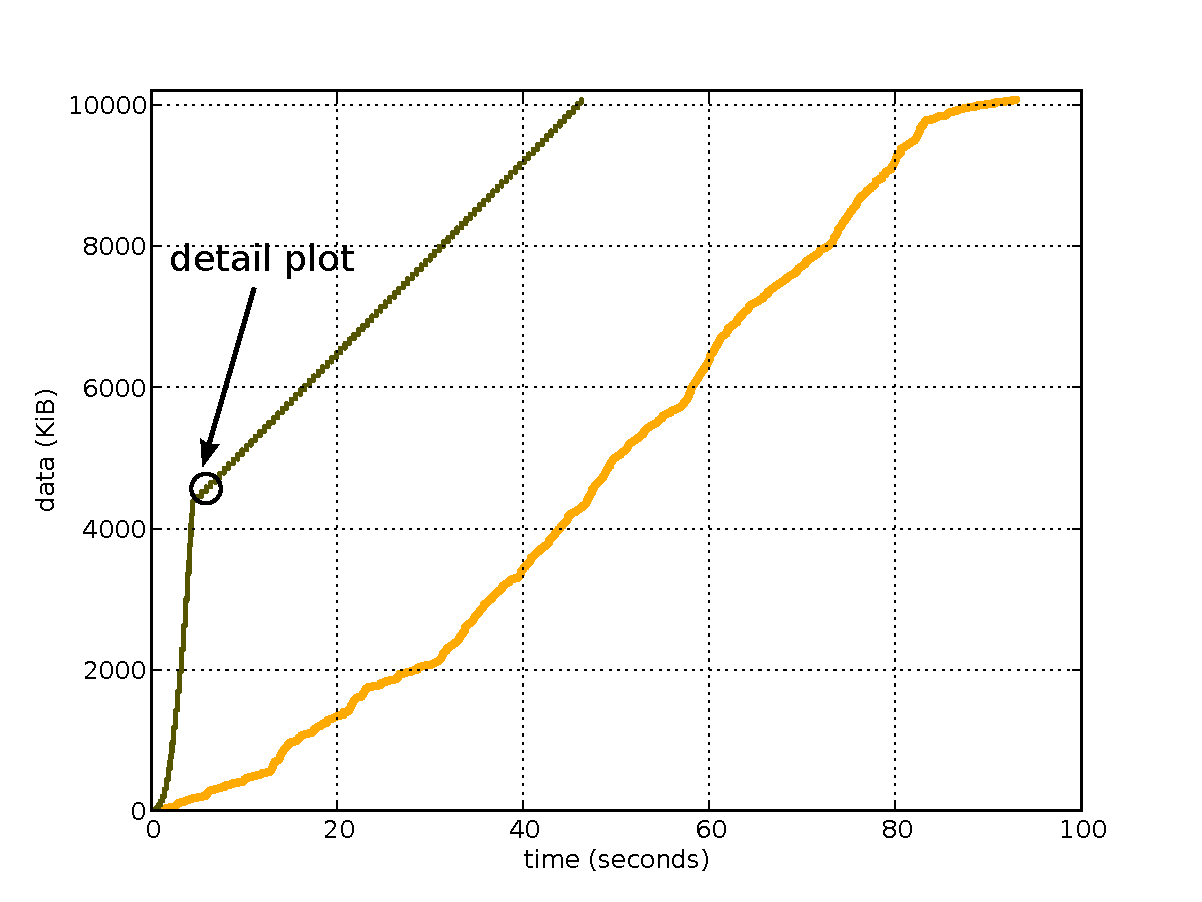
\includegraphics[width=\textwidth]{images/blocktransfer-mod.pdf}
                \caption{Overall graph.}
                \label{c3:fig:blocktransfer-overall}
        \end{subfigure}

        \begin{subfigure}[b]{0.90\textwidth}
                \centering
                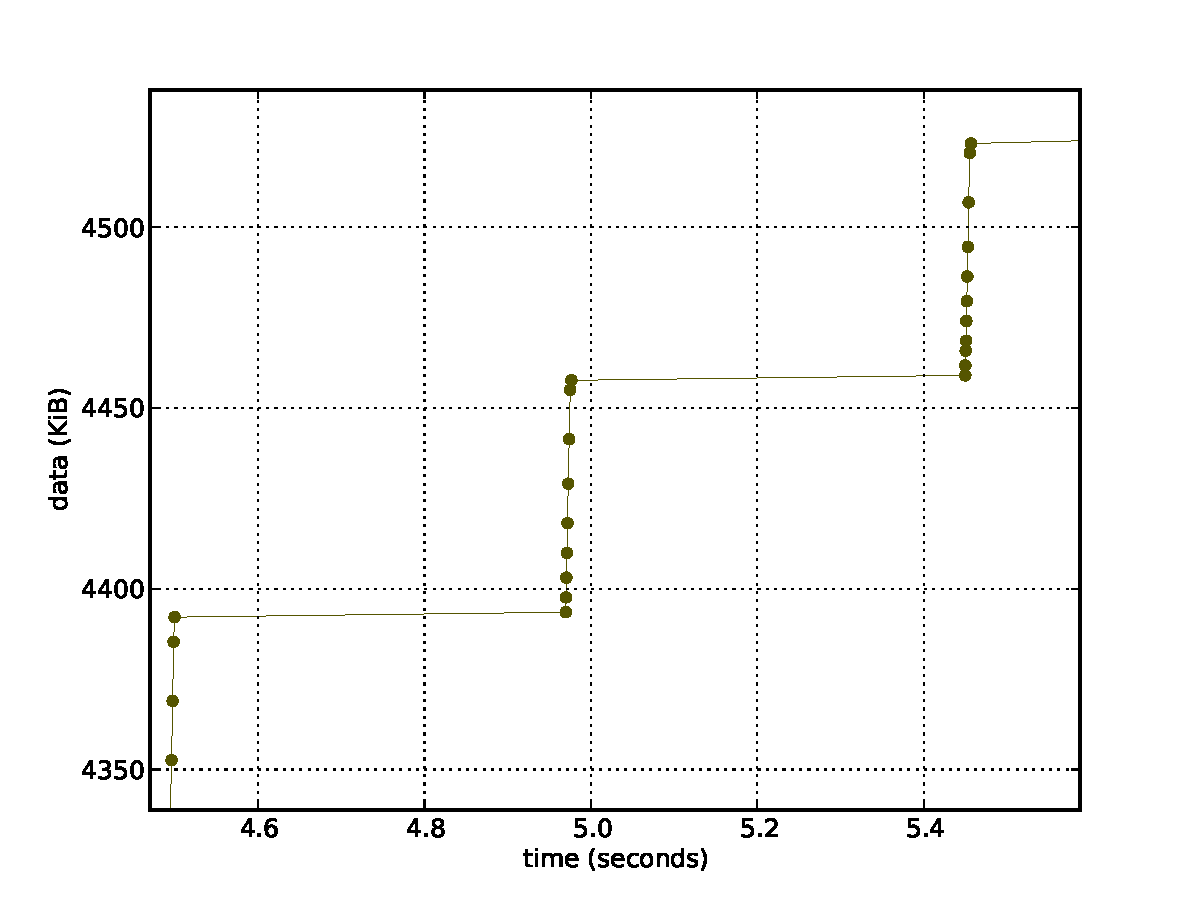
\includegraphics[width=\textwidth]{images/blocktransferdetail.pdf}
                \caption{Detail plot of the rate-limited block-sending phase.}
                \label{c3:fig:blocktransfer-detail}
        \end{subfigure}
\caption{Comparison of downloaded and consumed data volume revealing the pacing mechanism used by YouTube.}
\label{c3:fig:blocktransfer}
\end{figure}


The throttling method, also observed in \cite{alcock2011afcyt}, limits the transmission to a rate slightly above the average media bitrate, measurements and the \gls{URL} scheme indicates this to be a factor of the video bitrate of $1.25$. The rate limit is not constant, instead a ON-OFF block-sending scheme is facilitated. The scheme transmits short packet bursts, typically \SI{64}{\kibi\byte} in size, followed by long pauses as seen in Figure~\ref{c3:fig:blocktransfer}. The pause length between two bursts is set dynamically to reach the targeted bitrate on a larger time scale. The initial phase of the stream transmission is conducted unthrottled at line speed, presumably to allow for some pre-buffering to occur at the client media player. A possible reason for this server-side pacing is to avoid load spikes, with the added side effect of keeping the clients' buffer sizes in check.



%%
\paragraph{Firefox's HTML5 Player Strategy}

Video streaming can also be directly conducted with the Web browser, through the use of a HTML5 canvas element. The \gls{W3C} specifies the default technical process of HTMl5 video streaming in \cite{html5video} and essentially suggests a predictive strategy. Herein, the Web browser should estimate and correlate the transmission rate to the video bitrate. A property called ``autoplay'' uses this definition to start  playback of the associated video \enquote{as soon as it can do so without stopping}. The HTML5 strategy also allows to limit the buffer size through transmission pacing, negotiated with the server, and appropriately timed range requests.

The open-source Firefox browser represents an implementation of this specification and substantiates it further. The description of this strategy is based on Firefox's version 4.0 released in March 2011. Because it is an online algorithm which does not have global knowledge of the video and transmission speeds of any point in the future it has to estimate these.
To estimate the current and future rates, the moving average of the transmission rate $s_{MA}$ and the video bitrate $v_{MA}$ are calculated. The condition $c$ Firefox uses to start and resume the playback process is given in Algorithm~\ref{c3:alg:firefox}, with the buffered video duration $b_b$, and the duration spent buffering $b_T$.

\begin{algorithm}[htb]
    \centering
    \begin{algorithmic}
        \IF {$s_{MA} > v_{MA}$} 
          \STATE $c \gets ( b_b=20s \lor b_T=20s )$
        \ELSE
          \STATE $c \gets ( b_b=30s \lor b_T=30s )$
        \ENDIF 
    \end{algorithmic}
    \caption{Firefox playback (re-)start decision algorithm.}
    \label{c3:alg:firefox}
\end{algorithm}

 \begin{figure}[htb]
    \centering
    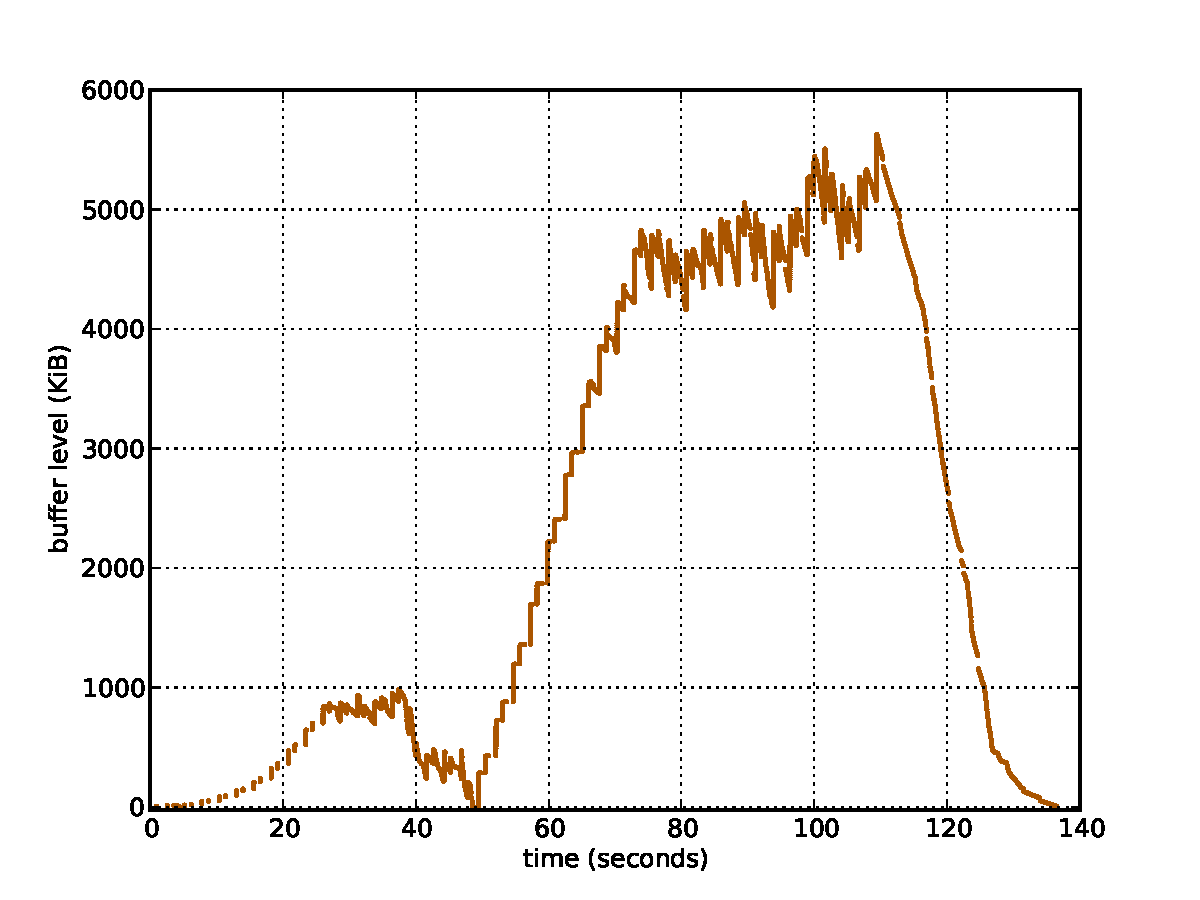
\includegraphics[width=0.9\textwidth]{images/bufferlevel-firefox-new.pdf}
    \caption{Sample buffer fill level for the Firefox 4 strategy, \SI{44}{\second} total stalling.}
    \label{c3:fig:bufferlevel-firefox}
\end{figure}


This approach is quite conservative and trades off long stalling periods for fewer stalls. The test case for our model is shown in Figure \ref{c3:fig:bufferlevel-firefox}. The playback starts only after a long waiting period and intermittent stalls cause a long buffering period. 
Due to the longer overall stalling time the player needs to buffer more data than other strategies. This may make it unsuitable for devices with sparse amounts of memory, e.g. mobile phones. On the other hand, could a large buffer also increase the chance of continuous playback in such scenarios with bad \gls{QoS}.


\paragraph{Adaptive streaming strategies}

Implementations for adaptive streaming players are again mostly proprietary and their behavior has to be derived from measurements. This is even true for adaptive streaming protocols, which have open specifications as these generally do not specify the player's behavior.

Microsoft's Silverlight player's strategy is described in \cite{BLTJ:BLTJ20505}. It employs a two-threshold model and rate estimations. When on of the thresholds is reached, the quality will be adjusted by one step upwards or downwards as long as the transmission rate is sufficient.

The buffering behavior of further protocol variants, including Adobe's \gls{HTTP} Dynamic Streaming, Apple's \gls{HTTP} Live Streaming and a sample implementation of \gls{DASH}, are investigated in \cite{Muller:2012:EDA:2151677.2151686,akhshabi2011experimental}.




% \begin{itemize}
% \item The player has been buffering data for at least 30 seconds.
% \item The player has already buffered an amount of data corresponding to 30 seconds of video.
% \item The video download has been completed.
% \item The moving average of the transmission rate is larger than the moving average of the video bitrate and the player has a safety buffer with 20 seconds of video data.
% \end{itemize}

% \begin{table}[htb]
%     \caption{Variables involved in buffering decisions.}
%     \label{c3:tbl:buffvars}
%     \centering
%     \begin{tabu}{|l|X[p]|} 
%     \hline
%     Variable & Description \\ \hline
%     $s_{MA}$ & Moving average of the transmission speed. \\
%     $v_{MA}$ & Moving average of the video bitrate. \\ 
%     $c$   & Condition upon which to start/resume playback. \\
%     $b_b$    & Amount of video data the buffer contains. \\
%     $b_T$    & Amount of time spent in non-playing buffering state. \\ \hline
%     \end{tabu}
% \end{table}

% used yt-delay/hPUGNCIozp0_delay_2500 1, spyder, color #aa5500
% data
% start delay 33s 
% flash 33.82s
% stalling 32.68s
% html5 as implemented in firefox 44s


%Which offers better quality to users? Some approaches (TODO: refs and explain how)

% Longer waiting time but very few stops. Stalling model definitely the shortest waiting time but stops too frequent with insufficient network conditions, i.e. can not really be used. Delayed playback requires total knowledge not available beforehand. Can maybe used with reduced information, bandwidth estimation, but this is essentially HTML5/Firefox.




%``application comfort'' time to skip, ...
%\subsubsection{Unreliable Streaming Metrics}
%... and why they mostly do not work / are not applicable.


%%%%%%%%%%%%%%%%%%%%%%%%%%%%%%%%%%%%%%%%%%%%%%%%%%%%%%%%%%%%%%%%%%%%%%%%%%%%%%%%
%!TEX root = ../../dissertation.tex
%%%%%%%%%%%%%%%%%%%%%%%%%%%%%%%%%%%%%%%%%%%%%%%%%%%%%%%%%%%%%%%%%%%%%%%%%%%%%%%
\section{Load Model Queuing Simulation} 
\label{c4:sec:simulation}

As discussed, the solvability of a non-stationary Erlang loss system is very limited. To better tackle this, a simulative approach can be taken. Depending on the level of detail, different types of simulations are available.

Here, a queuing simulation is used to ascertain the blocking probability and tunnel serving slot utilization from the model using the fitted distributions from the trace.


%%%%%%%%%%%%%%%%%%%%%%%%%%%%%%%%%%%%%%%%%%%%%%%%%%%%%%%%%%%%%%%%%%%%%%%%%%%%%%%
\subsection{Queuing Simulation Implementation}

The queuing simulation is implemented on the basis of a \gls{DES}. Instead of reproducing continuous time, this simulation is a series of discrete events. Time is advanced only at these events. 

A queuing model can be easily represented in a \gls{DES}.  Each tunnel request arrival is modeled as a discrete event. When such an event occurs, three processes are executed. The first process draws a random number from a \gls{PRNG} mapped to \gls{IAT} exponential distribution to schedule the next arrival event. Secondly, the serving units are checked for any free units. If one is found, it will now be occupied. Else, this arrival will be marked as rejected and the third action skipped. This third process now determines the length of the tunnel using another \gls{PRNG} adjusted to the serving time distribution to schedule the event in which the tunnel exits the system.

This model was implemented on the basis of version 3.0 of the \textit{SimPy}\footnote{\url{https://simpy.readthedocs.org/}} package, which is a Python \gls{DES} framework that provides the basic event and scheduling infrastructure. On top of this a base \gls{GGSN} class was constructed, managing the arrival of tunnel events and the scheduling of the service ending events. Specific classes for the traditional (i.e. monolithic) and virtualized (called ``multiserver'' in the code) nodes respectively exist.\footnote{The implementation is also publicly available at \url{https://github.com/fmetzger/ggsn-simulation/} as a reference.}


%%%%%%%%%%%%%%%%%%%%%%%%%%%%%%%%%%%%%%%%%%%%%%%%%%%%%%%%%%%%%%%%%%%%%%%%%%%%%%%
\subsection{Description and Design of the Individual Experiments}

To match the measurement data the simulation time is set to be \SI{7}{\day} in all simulation scenarios. The initial \SI{60}{\minute} of each experiment are considered to be the transient phase and are afterwards deducted from the results. Ten replications of each scenario were performed. All depicted error bars show the \SI{95}{\percent} confidence intervals across the experiments.

The first experiment was conducted to investigate the normalized baseline load a monolithic \gls{GGSN} experiences using the presented model. Using this, a maximum to the number of concurrent tunnels and the correlation to the blocking probability and tunnel rejection rate can be established. The effects of scaling up, improving the hardware capabilities of the single node, can thus be investigated.

Based on these results, the virtualization and scaling out effects in the virtualized, \gls{GGSN} model are examined. In order to study the feasibility of this approach the performance indicators of the virtual \gls{GGSN} are compared to the baseline established in the first experiment. To this end, the virtual \gls{GGSN} is simulated in configurations varying the number of instances and supported concurrent tunnels per instance.

In a final experiment the startup and shutdown duration of virtual instances and the life cycle management of these instances are additionally taken into account. Although the boot duration of modern \glspl{os} and \glspl{VM}, especially on current hardware with flash storage, is significantly lower than it has been in the past, there is still a delay. This could cause further blocking if the load balancer does not account for this. But the more generously the balancer starts instances in advance the smaller the virtualization efficiency gain, especially the energy consumption, will be become. For this reason, the number of active instance is a relevant performance metric in the virtual \gls{GGSN} model.

The experiment varies the boot delay and implements a very simple load balancer rule as baseline. The rule keeps at least one empty instance running in reserve at all times and deactivates instances, when two running instances are completely unused. As this is very generous, virtualization blocking should only occur in cases of very small instances or very rapid arrivals. Realistic provisioning rules can improve on this quite easily. But even this simplistic approach already serves to demonstrate potential benefits.


%%
\subsubsection{GGSN Load, Capacity, and Scaling}

First, with the help of the \glspl{IAT} and duration of tunnels calculated in the dataset evaluation, the monolithic \gls{GGSN} model is studied. While these traces provided information on the frequency of new tunnels and the duration they remain active, no reliable information on the number of required supported concurrent tunnels for a given arrival rate could be deduced. 
This experiment evaluates arbitrary values for the \gls{GGSN} tunnel capacity and determines the resulting blocking probability such that a suitable value can be found. This is a typical task in a dimensioning process.

\begin{figure}[htb]
	\centering
	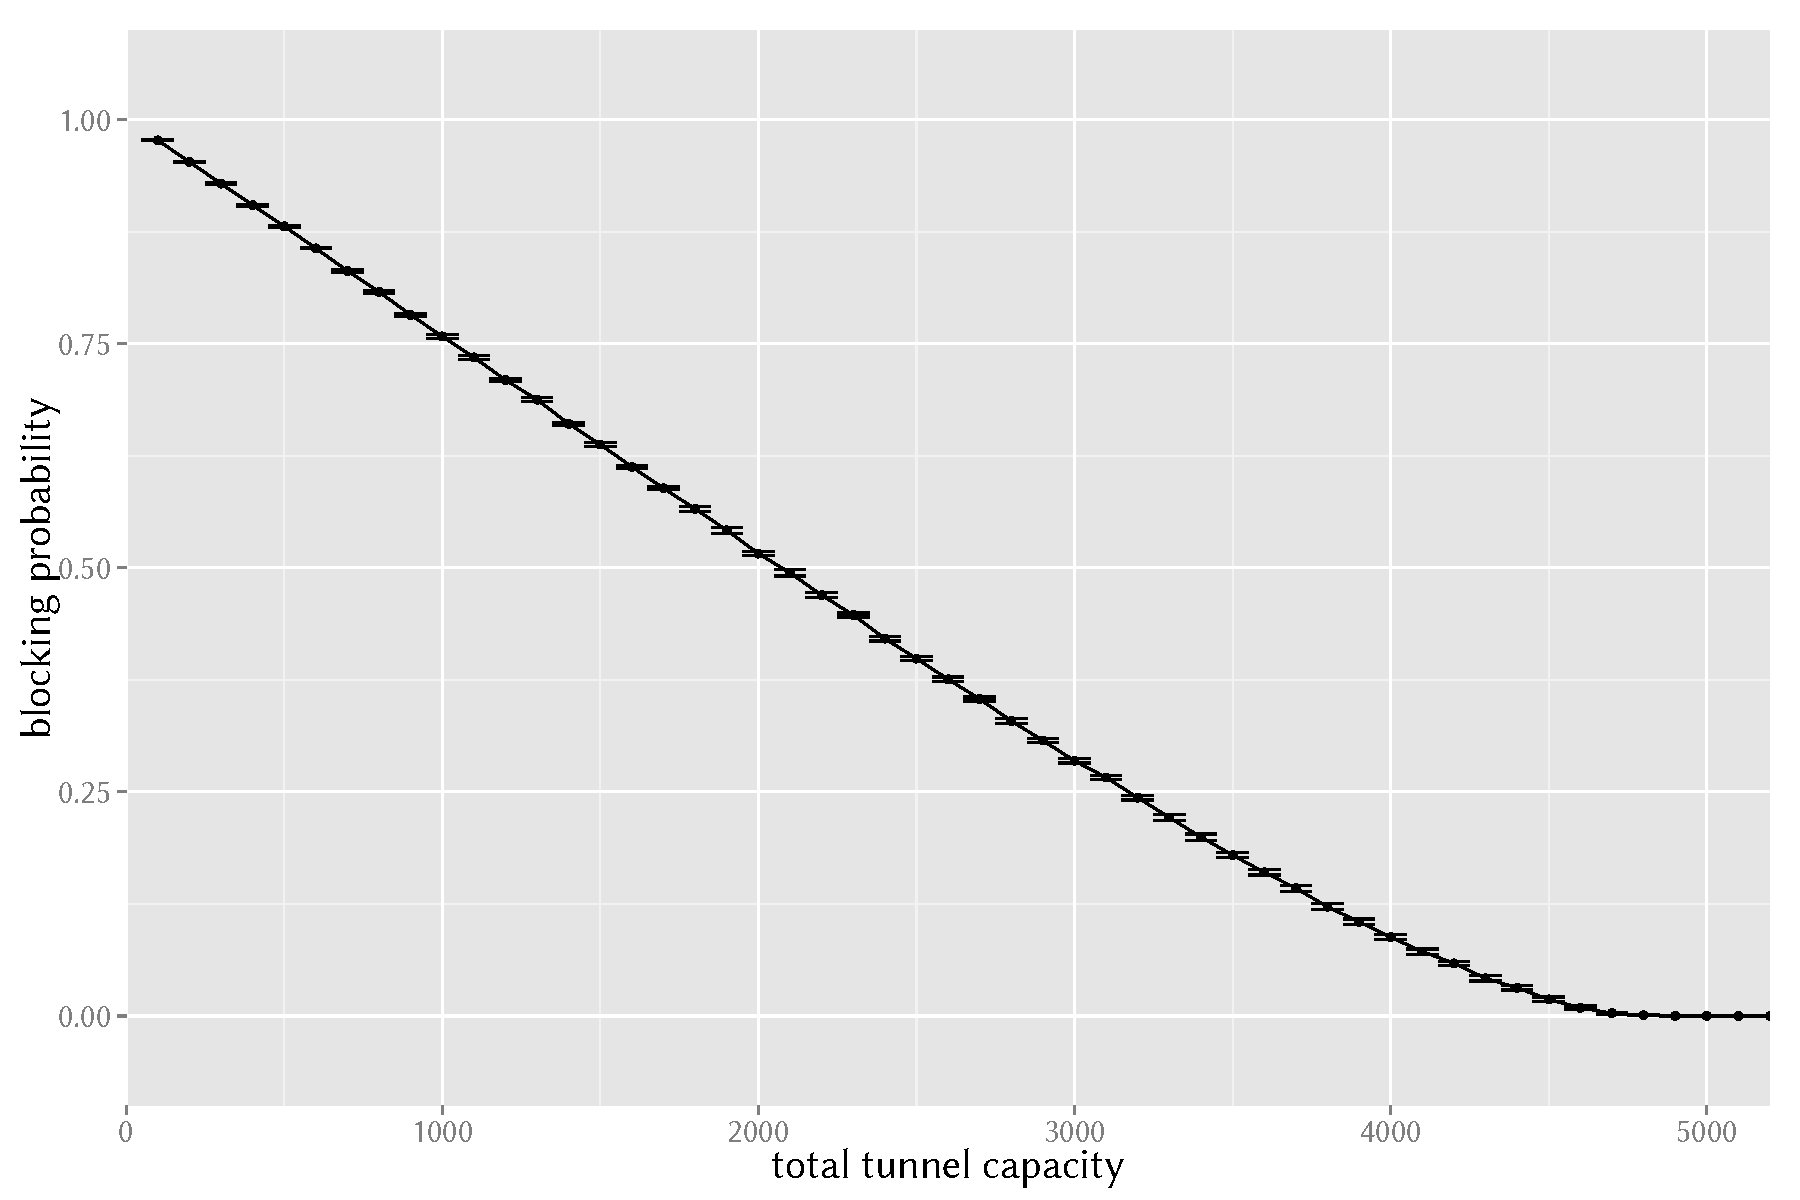
\includegraphics[width=0.9\textwidth]{images/R-monolithic-blocking.pdf}
	\caption{Impact of the number of supported parallel tunnels on the blocking probability for the traditional \gls{GGSN} model. For each scenario the mean and \SI{95}{\percent} confidence intervals of all simulation replications are shown.}
\label{c4:fig:traditional_blocking}
\end{figure}

Figure~\ref{c4:fig:traditional_blocking} studies this impact of the maximum supported number of concurrent tunnels $n$ on the blocking probability $p_B$. $n$ is incrementally increased in steps of \numprint{100} tunnels from \numprint{0} to \numprint{5500}. As expected, the blocking probability decreases with the number of supported tunnels. An almost linear correlation can be observed in the larger part of the graph with a small convergence phase shortly before reaching $p_B=0$. For the normalized inter-arrival no blocking is occurring if a capacity of \numprint{5000} concurrent tunnels is allocated to the \gls{GGSN}.

\begin{figure}[htb]
	\centering
	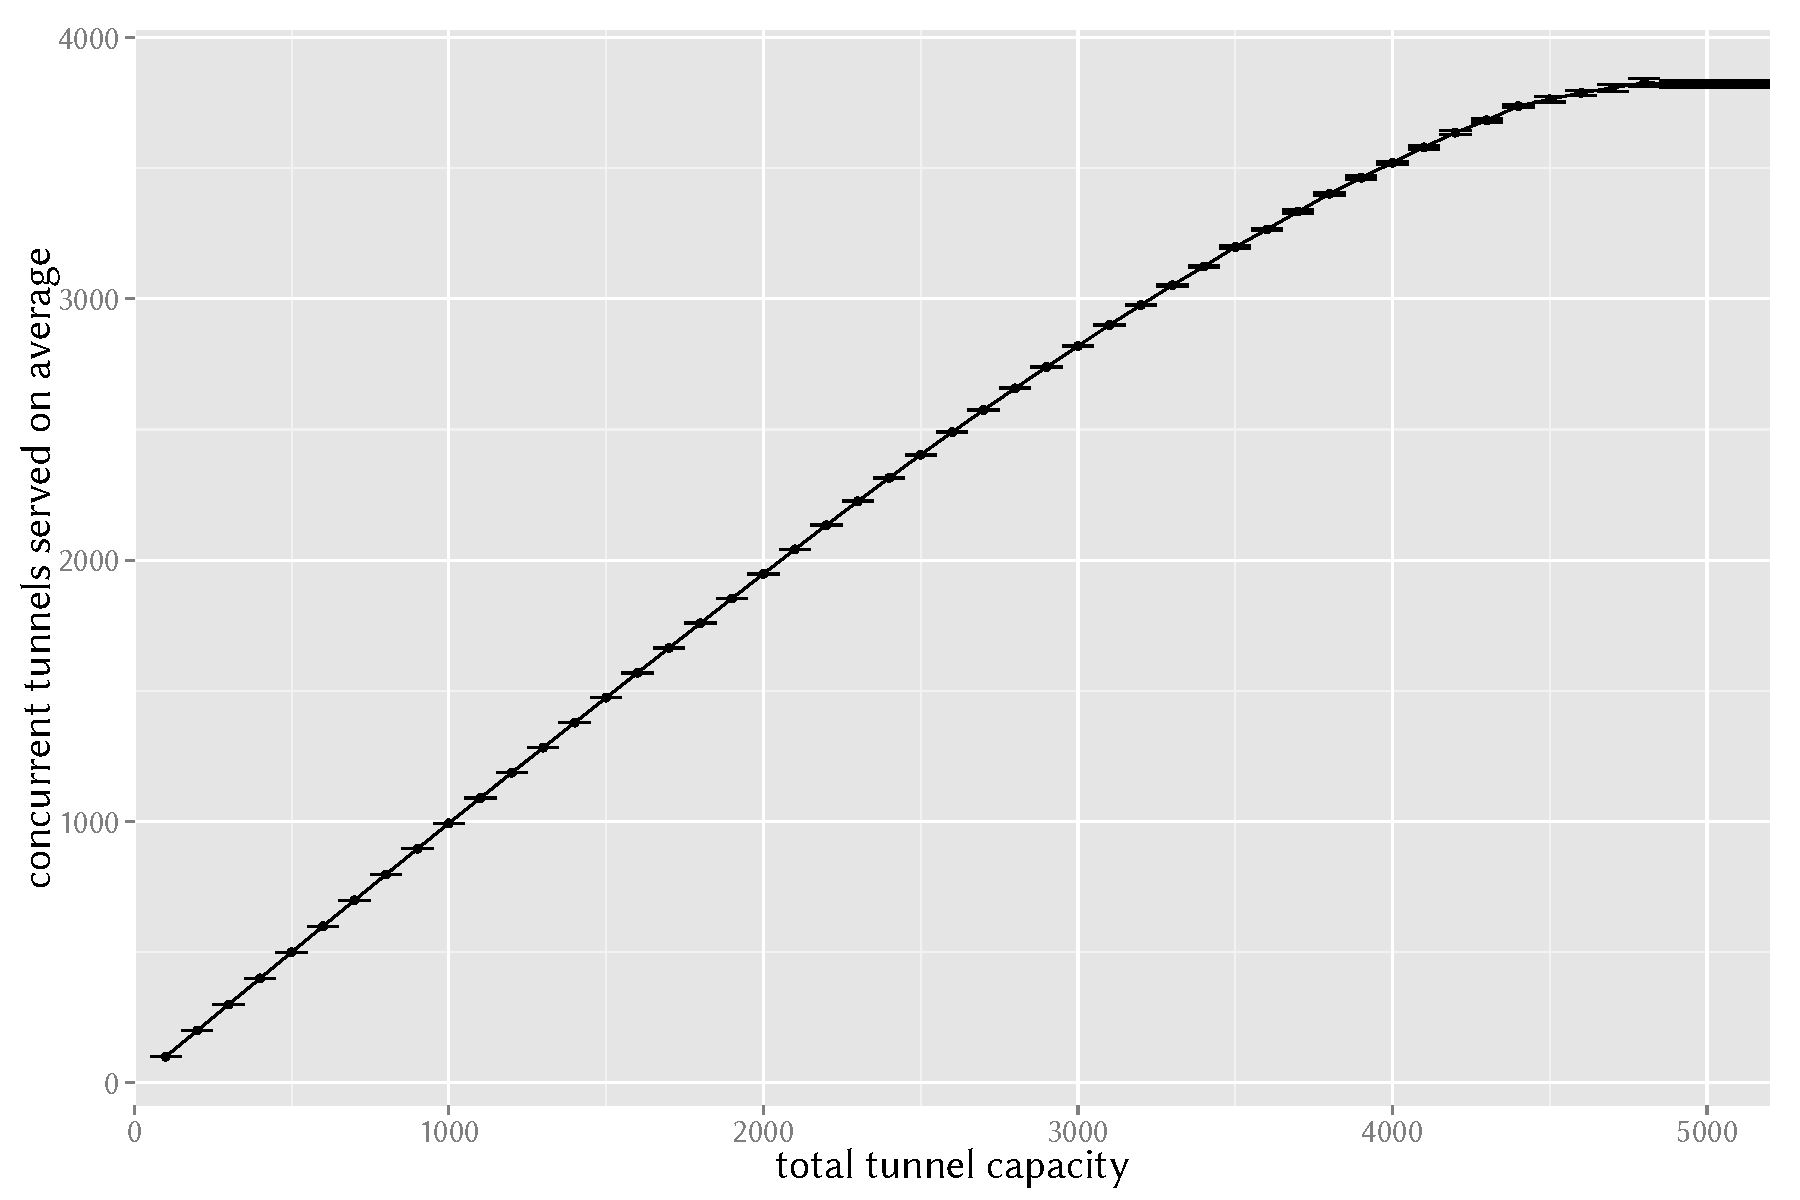
\includegraphics[width=0.9\textwidth]{images/R-monolithic-tunnelusage.pdf}
	\caption{Mean number of tunnels concurrently served by the \gls{GGSN} for incrementally increasing capacity. For each scenario the mean and \SI{95}{\percent} confidence intervals of all simulation replications are shown.}
\label{c4:fig:traditional_tunnelusage}
\end{figure}

A similar picture is also evident in the number of tunnels served by this \gls{GGSN} in the same scenario as shown in Figure~\ref{c4:fig:traditional_tunnelusage}. For the first half of the experiments the \gls{GGSN} is loaded to its limit. Only when the capacity reaches \numprint{4600} can the normalized arrival rate be fully served, which surmounts to about \numprint{3820} tunnels on average in the system. Both results are stable across all simulation runs as the confidence intervals display. For the purpose of network dimensioning the results can be easily scaled up from the normalized arrival rates to the actual ones in the network in question.


%%
\subsubsection{Virtualization Impact and Gain}

A similar experiment can be set up for the virtual \gls{GGSN} model. Learning from the monolithic model, these follow-up simulations can be tuned to the same total tunnel capacity in advance. The only difference is that the tunnel capacity is now spread out evenly between the virtual \gls{GGSN} instances. The experiment tests different amounts for the total number of virtual instances, ranging from \numprint{1}, which represents the monolithic architecture, up to \numprint{100} instances in steps of \numprint{10}.

\begin{figure}[htb]
	\centering
	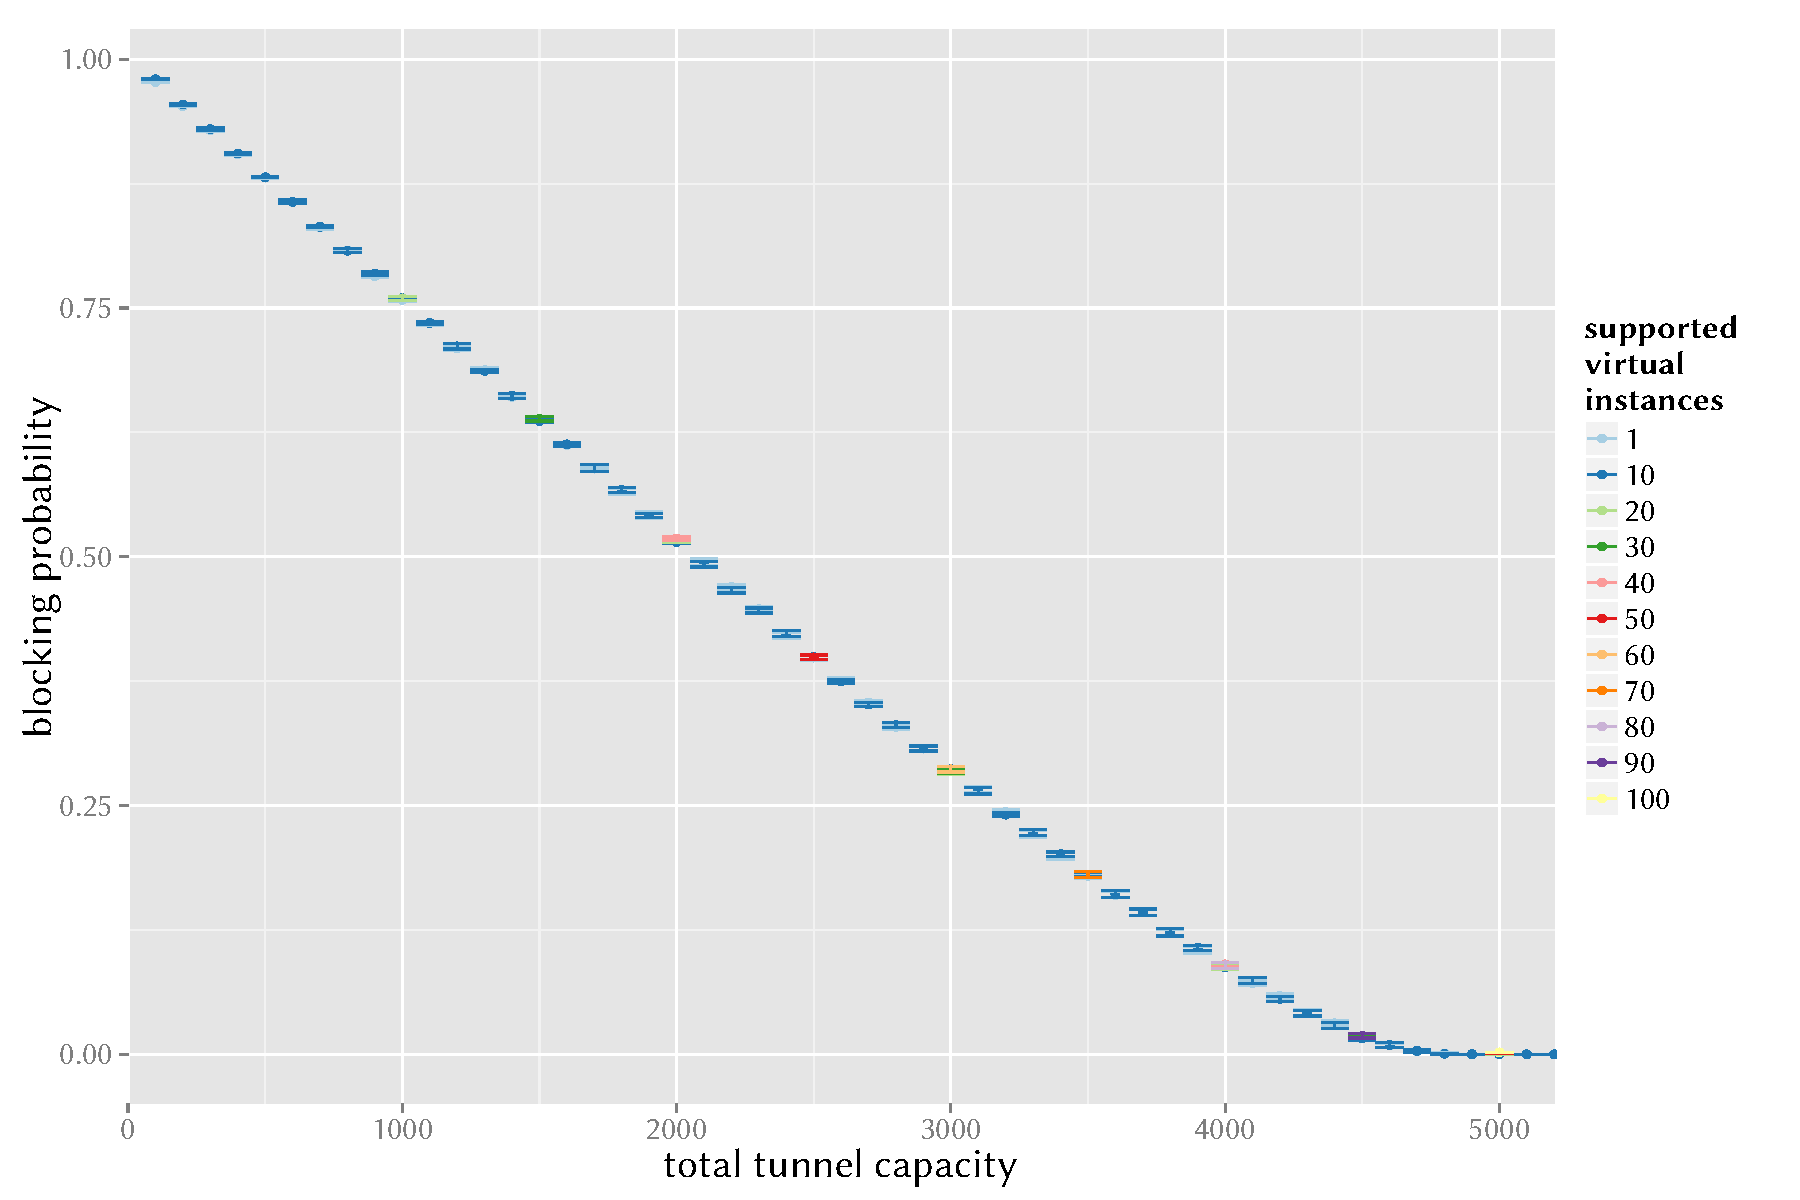
\includegraphics[width=0.9\textwidth]{images/R-virtualized-blocking.pdf}
	\caption{Comparison of the mean blocking probability of various server configurations with \SI{95}{\percent} confidence intervals. The x axis depicts the summary capacity of all virtual instances in the experiment.}
\label{c4:fig:virtualized_blocking}
\end{figure}

\begin{figure}[htb]
	\centering
	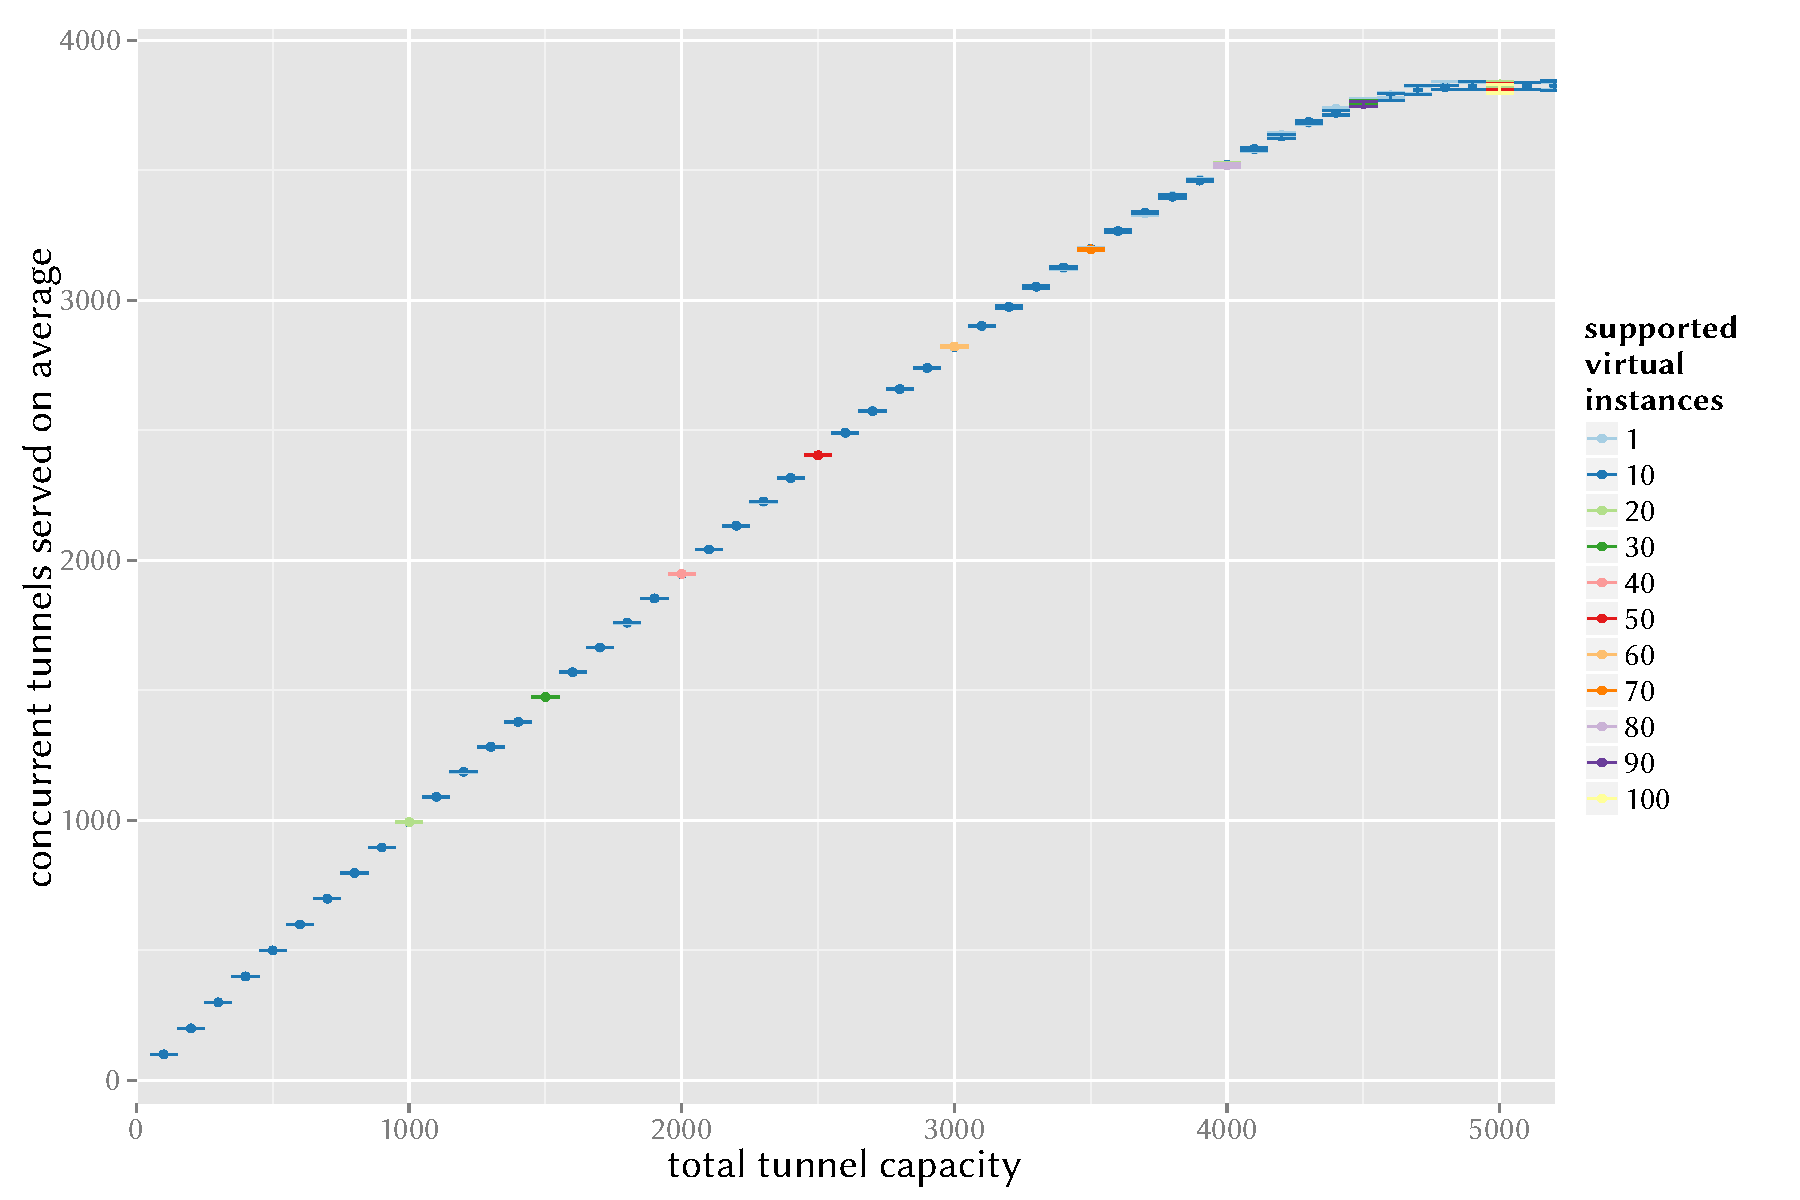
\includegraphics[width=0.9\textwidth]{images/R-virtualized-tunnelusage.pdf}
	\caption{Comparison of the mean tunnel occupation of various virtualization configurations with \SI{95}{\percent} confidence intervals.}
\label{c4:fig:virtualized_tunnelusage}
\end{figure}

Figures~\ref{c4:fig:virtualized_blocking} and \ref{c4:fig:virtualized_tunnelusage} demonstrate the results in terms of $p_b$ and concurrent tunnels served overlaid onto the base monolithic scenario's results. No large difference in the results can be seen and the virtualized \gls{GGSN} model behaves no worse than a single large node model.

\begin{figure}[htb]
	\centering
	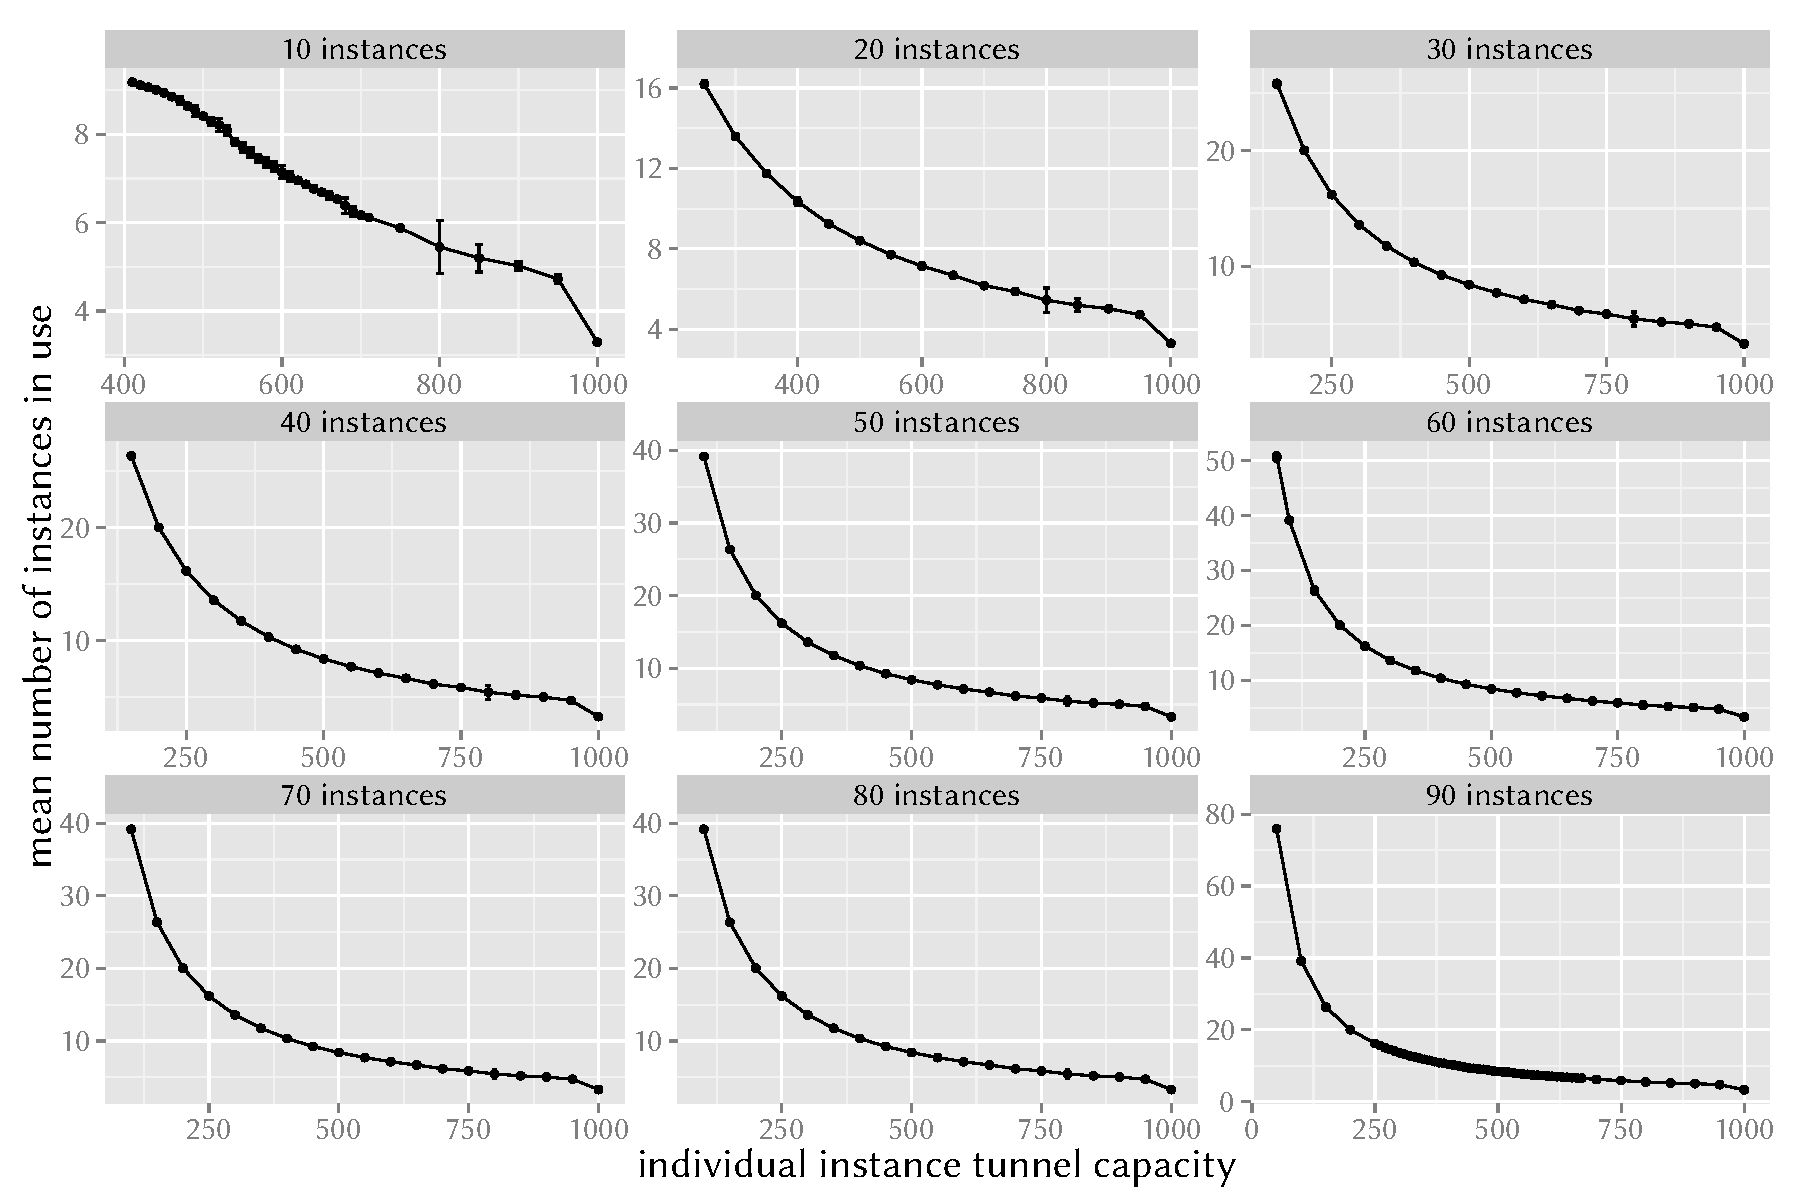
\includegraphics[width=0.9\textwidth]{images/R-virtualized-mean-instanceusage.pdf}
	\caption{Mean instance usage of various virtualization configurations. A higher number of total instances results in a finer granularity of scaling and energy efficiency as more instances can be kept shut down.}
 \label{c4:fig:res-instance-usage-mean}
\end{figure}

But the possible effects of an increased number of instances need to be investigated further. One goal in virtualization is the increase of energy efficiency. This can be achieved by having turned on just as many instances as needed and not more, thus scaling the system to its current load. 

Therefore, Figure~\ref{c4:fig:res-instance-usage-mean} takes a look at scenarios with nine different instance pools and varying tunnel capacities for each instance. Each setup is compared by the mean number of active instances during the one-week course. The bigger the instances' capacity becomes the less instances need to be active. An actual \gls{GGSN}, even a virtualized one, would need to be dimensioned in such a way to keep the total overhead low. It was already determined that, with the assumed normalized arrival rate, a capacity of \numprint{5000} tunnels is sufficient in order to achieve a blocking probability close to zero. Keeping the setup at this minimum capacity and taking a look at the results in the figure, a good portion of the instances, usually around \SI{20}{\percent}, can still be kept turned off.

\begin{figure}[htb]
	\centering
	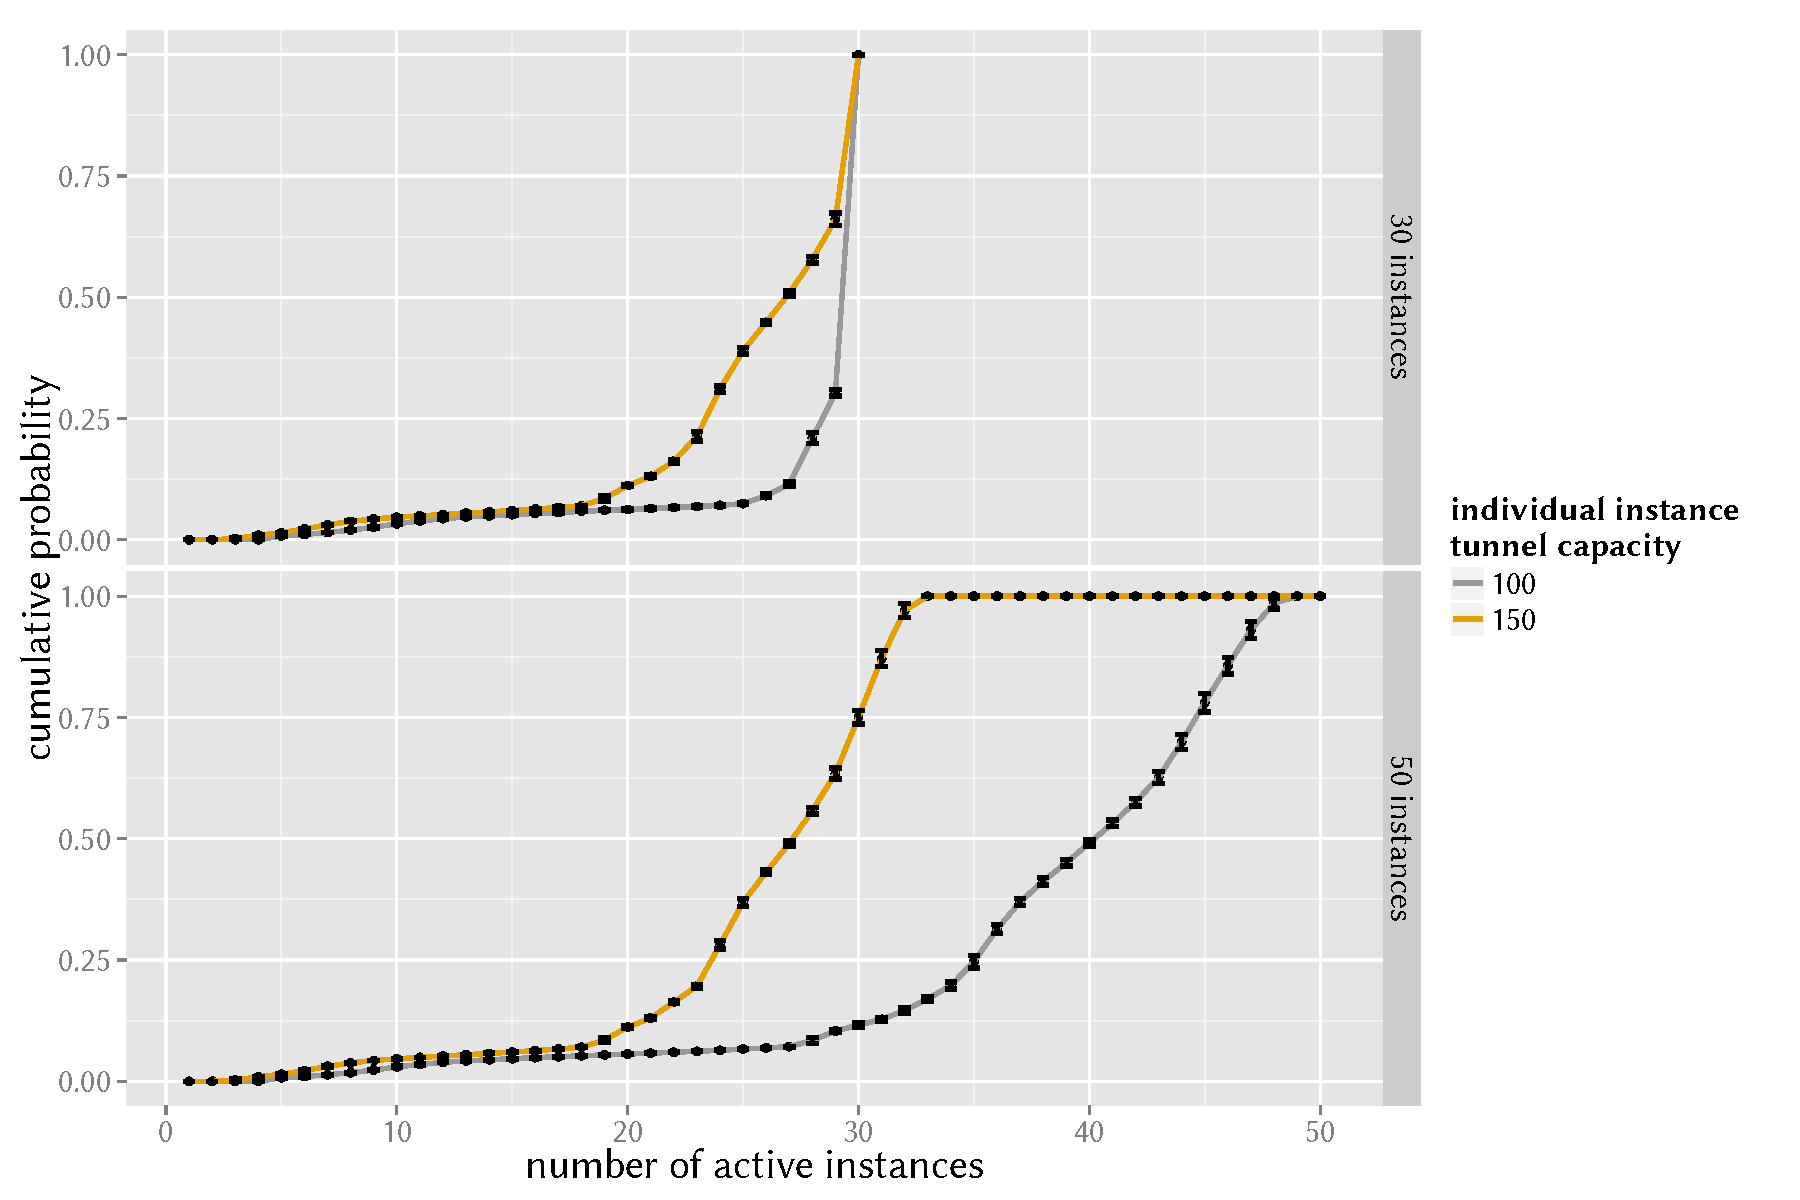
\includegraphics[width=0.9\textwidth]{images/R-virtualized-instanceuse.pdf}
	\caption{Impact of the maximum number of tunnels and number of instances on the number of active instances in the virtual \gls{GGSN} model.}
\label{c4:fig:virtualized_instanceuse}
\end{figure}

To get into more detail, Figure~\ref{c4:fig:virtualized_instanceuse} displays the distribution of the portion of time a specific number of instances was active. Depicted are four configurations that differ in their total number of instances and their tunnel capacity. The setup with \numprint{30} instances with \numprint{100} capacity was clearly overwhelmed with the arrival rate and all \numprint{30} instances were active over \SI{70}{\percent} of the time. Only when \numprint{150} were allowed the virtualization benefits come into effect and more instances are able to sleep. Similar observations can be made in the \numprint{50} instance case.  Here, the \numprint{100} tunnel scenario is already equipped to handle the tunnel arrival rate and can scale back its active instances quite well, below \numprint{40} instances half the time. The final configuration with a \numprint{150} tunnel capacity is clearly overdimensioned here with no more than \numprint{33} of the \numprint{50} instances ever being active.

\begin{figure}[htb]
	\centering
	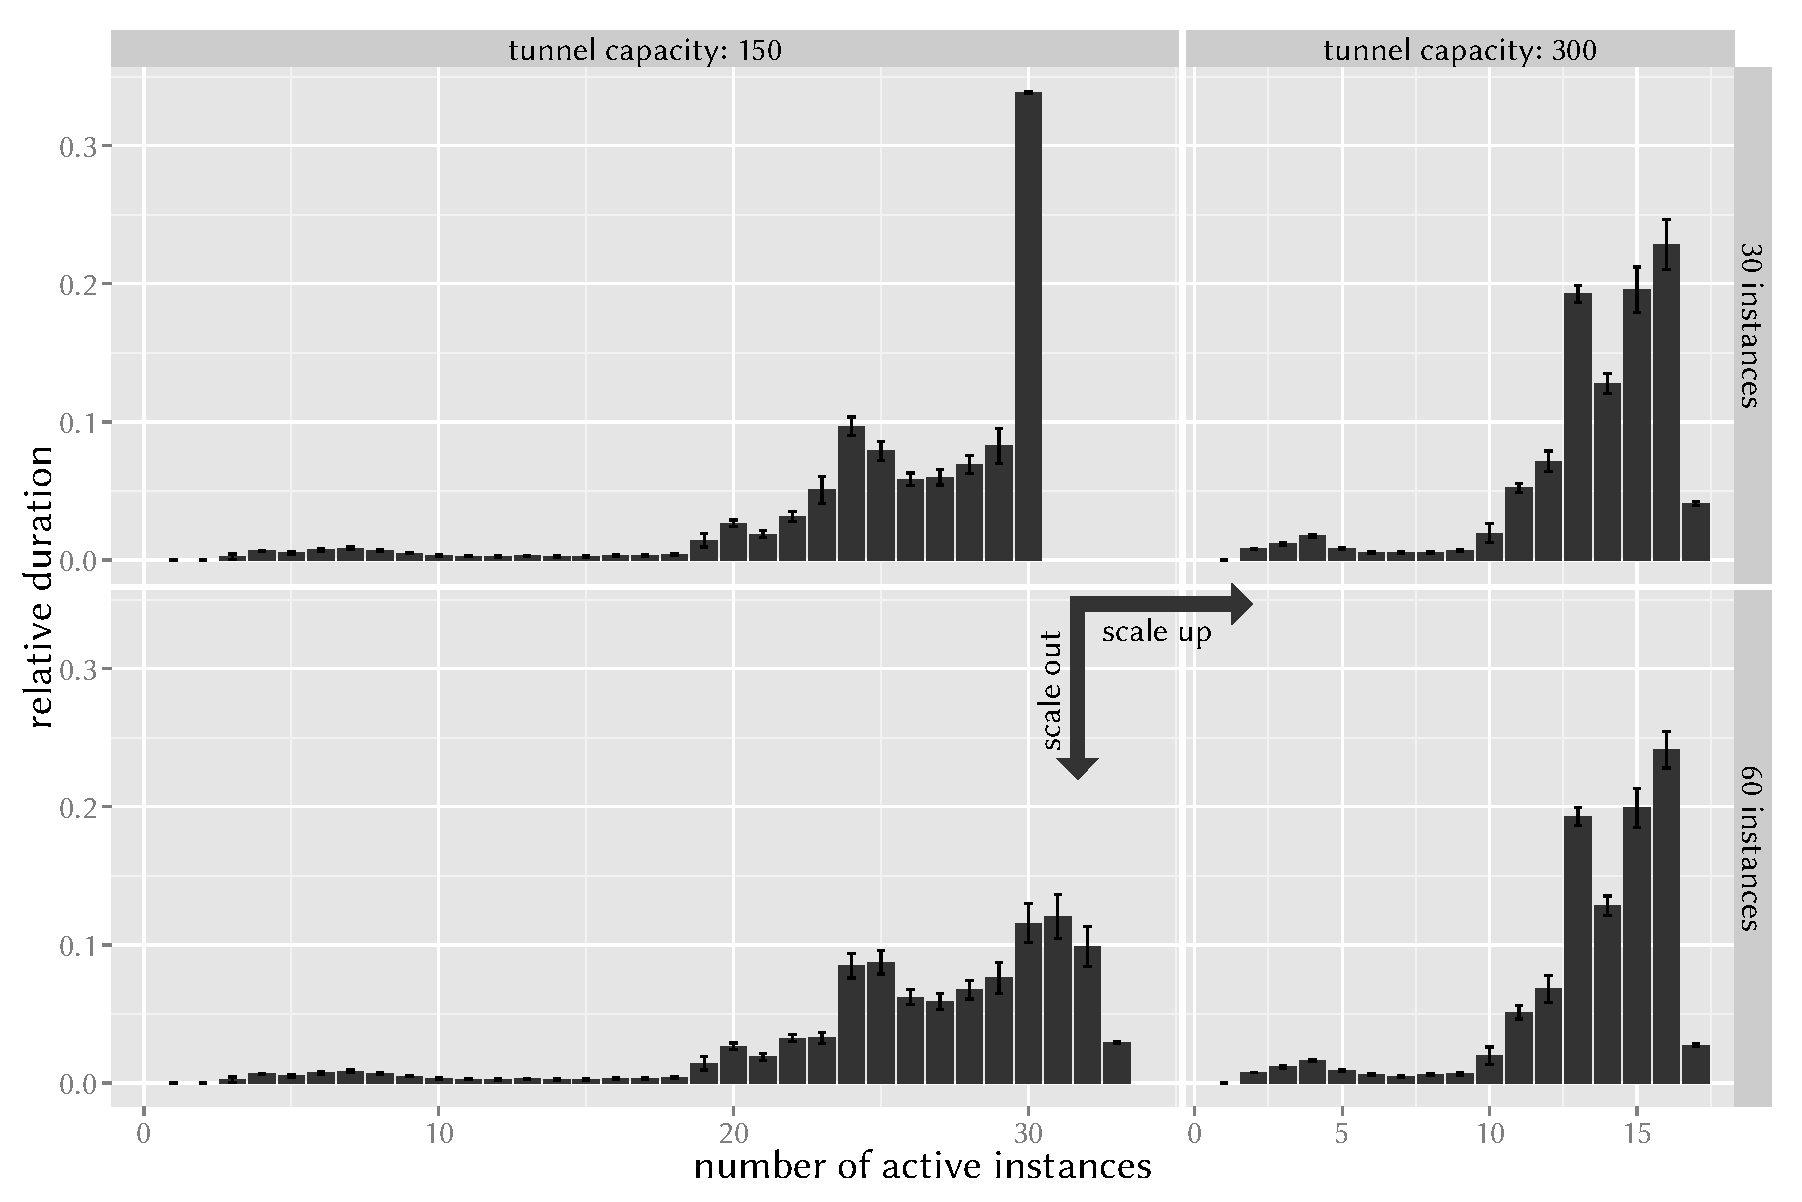
\includegraphics[width=0.9\textwidth]{images/R-virtualized-instanceuse-barplot.pdf}
	\caption{Resource usage from a select maximum instances and tunnel capacity combination, displaying the capability to scale up and out.}
\label{c4:fig:res-usage-barplot}
\end{figure}


Looking at these scenarios and additionally Figure~\ref{c4:fig:res-usage-barplot} from a network dimensioning perspective, two distinct pathways to scale in the virtualized \gls{GGSN} model are revealed. To reach the desired tunnel capacity either the number of instances or the instance's tunnel capacity can be increased. The latter represents the classical \textit{scaling up}. But virtualization also opens up the new path of \textit{scaling out} by increasing the number of instances. Through this, scaling can be become easier and cheaper as existing machines need not be replaced any more.


%%
\subsubsection{Virtual Instance Life Cycle Management Impact}

A final aspect to be investigated in the experiments is the potential increase of the blocking probability in virtualized scenarios when compared to the monolithic base. In theory, virtualization can incur additional overhead which would represent itself as an increase in $p_b$. In the given model the overhead can stem from the hypervisor and its scheduling  and lifecycle management strategies in conjunction with the instances' boot delay. 

The somewhat simplistic hypervisor strategy in this simulation was already discussed above and should give an upper limit on the impact on the blocking probability. This strategy is fixed, but the instance boot duration gets changed to analyze the impact. Values between \SI{20}{\second} and \SI{5}{\minute} are considered and should reasonable represent real-life systems of a wide variety.

\begin{figure}[htb]
	\centering
	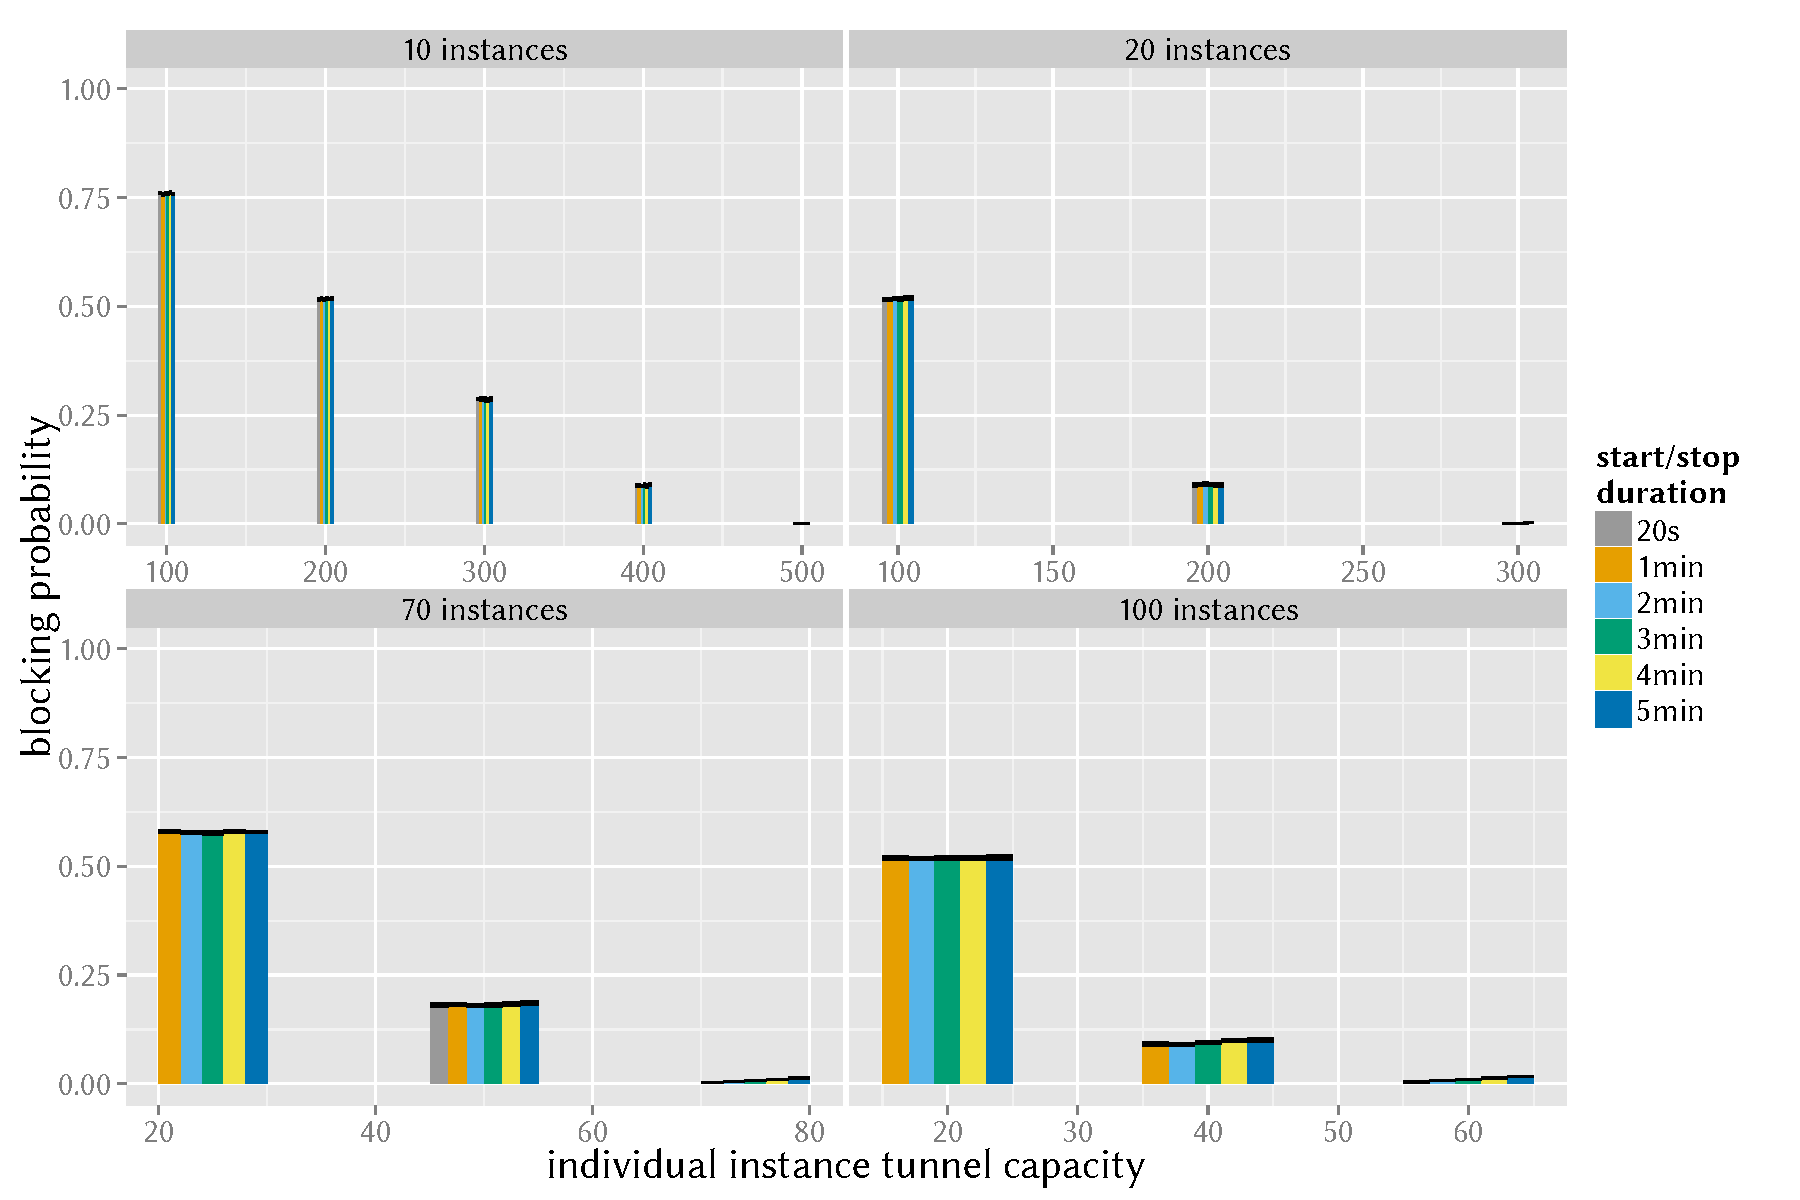
\includegraphics[width=0.9\textwidth]{images/R-virtualized-startstop-blocking-barchart.pdf}
	\caption{Influence of the boot and shutdown time on the blocking probability.}
\label{c4:fig:blockprob-startstop-barchart}
\end{figure}

Figure~\ref{c4:fig:blockprob-startstop-barchart} compares a number of instance and tunnel capacity scenarios on basis of their instance boot duration. In most scenarios there is almost no increase in the tunnel blocking probability. Only in cases with very many but small instances, where a lot of instance churn will occur, an increase can be noticed for higher boot durations.

\begin{figure}[htb]
	\centering
	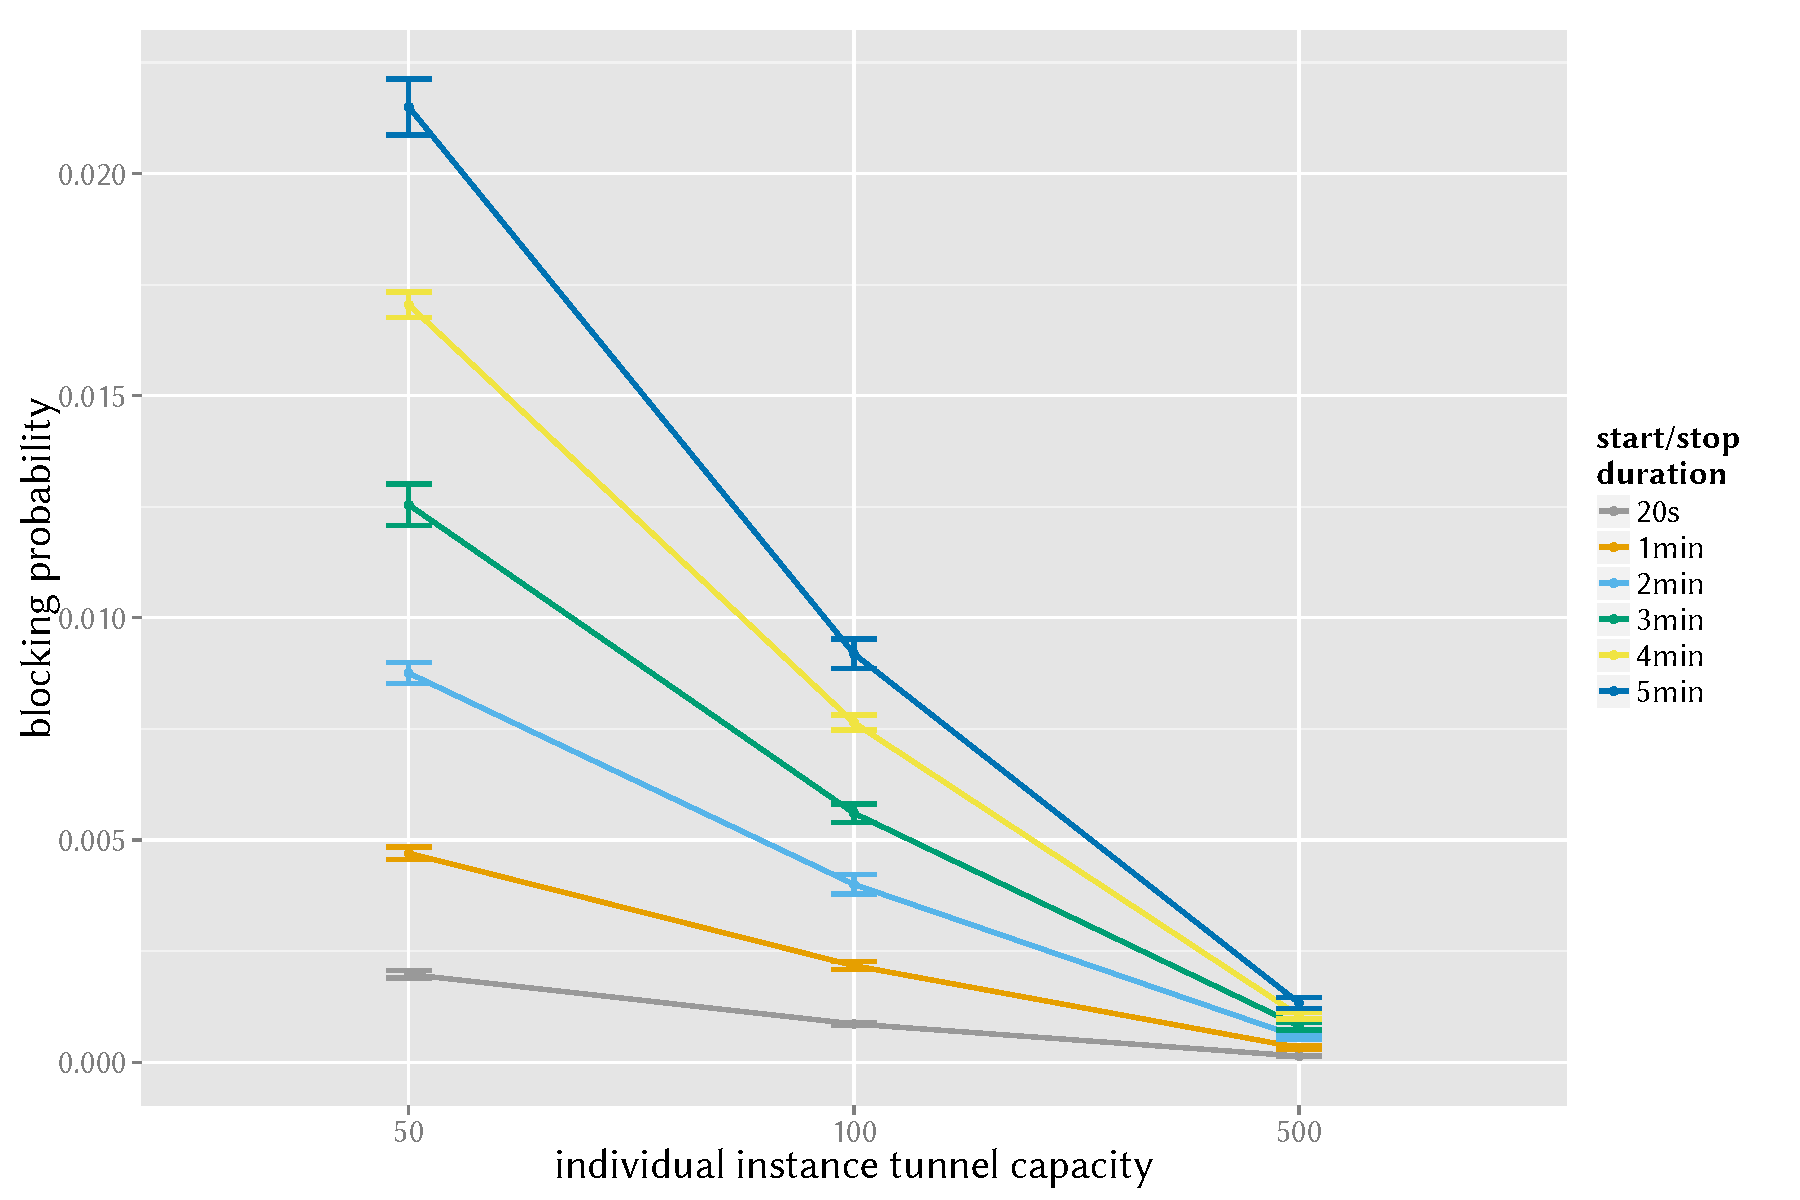
\includegraphics[width=0.9\textwidth]{images/compare-maxinstances-block.pdf}
	\caption{Influence of start up and shut down time on blocking probability with regard to different numbers of instances.}
\label{c4:fig:compare_maxinstances_block}
\end{figure}

Figure~\ref{c4:fig:compare_maxinstances_block} investigates this increase in more detail and shows the blocking probability of one select scenario. Here, the system supports \numprint{5000} tunnels in total with differing individual instance capacity of \numprint{50}, \numprint{150}, and \numprint{500}. In each case the start and stop down duration is changed between \SI{1}{\minute} and \SI{5}{\minute}. The increase in blocking probability in relation to both the instance capacity as well as the start duration can be easily observed.

This can be partially attributed to the hypervisor and its simplistic scheduling  and lifecycle management strategies in the simulation. If a low capacity instance with a long start time is activated, there is a high probability that the system will quickly expend its capacity again.
A potential conclusion is that choosing larger instance capacities decreases the blocking probability at the cost of energy efficiency (because less instances can stay turned off).

\begin{figure}[htb]
	\centering
	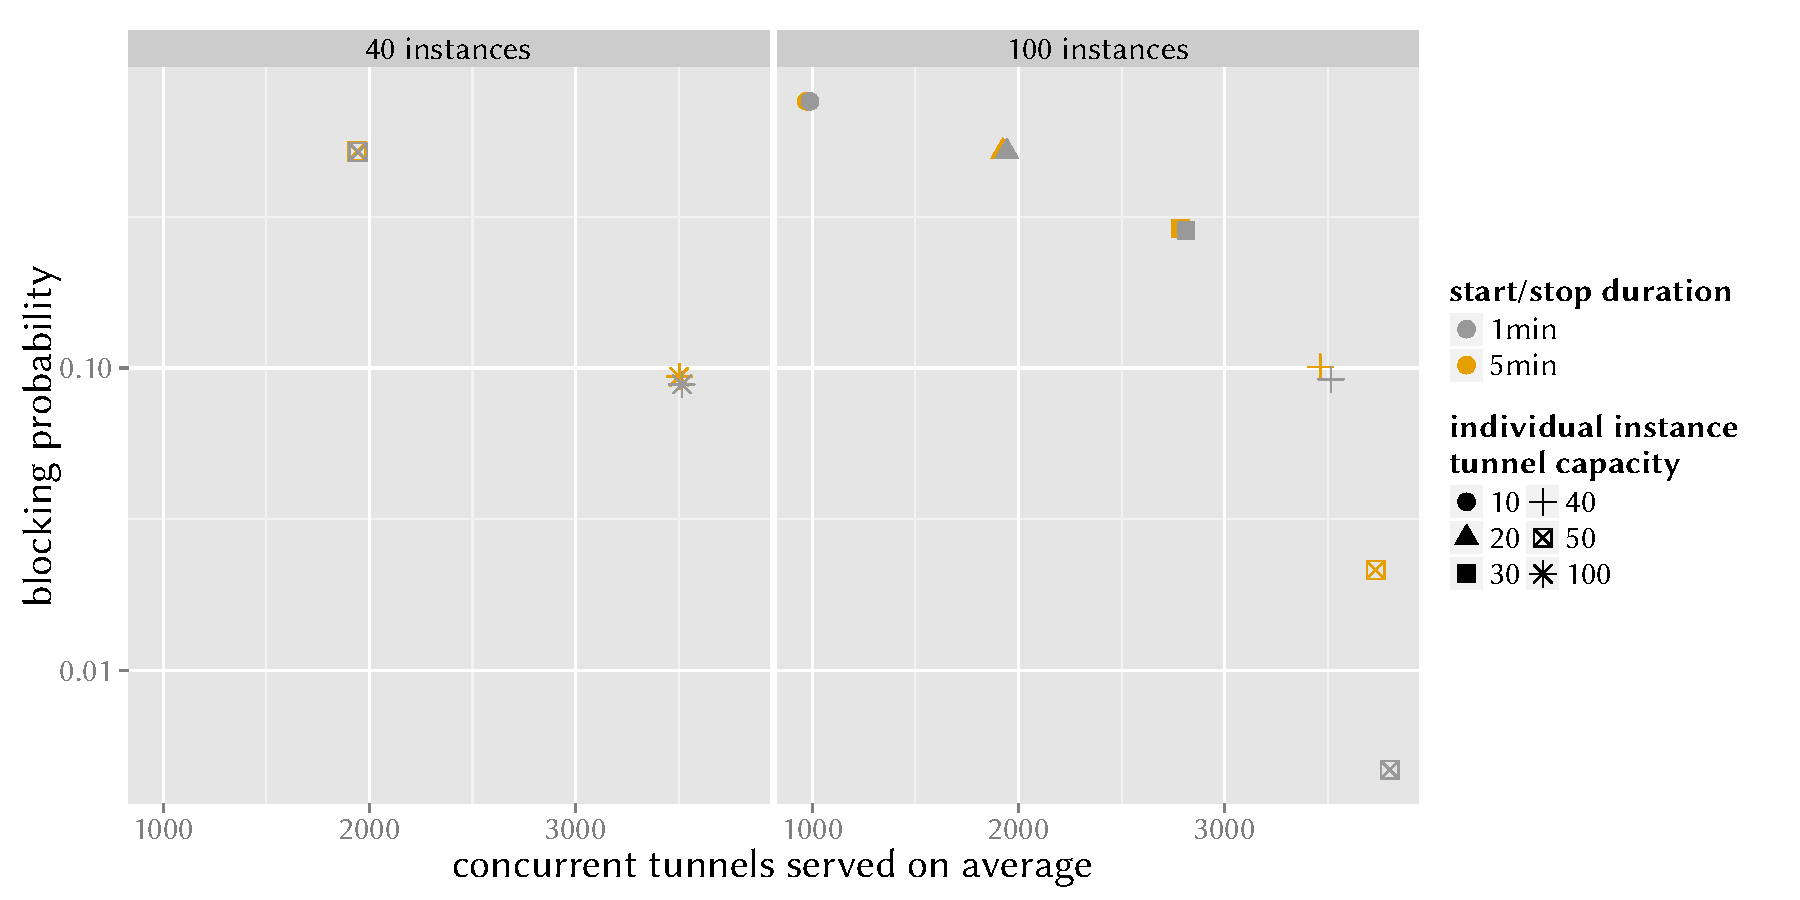
\includegraphics[width=0.9\textwidth]{images/R-virtualized-startstop-tunnelusage-blocking-comparison.pdf}
	\caption{Trade-off between blocking probability and mean resource utilization with regard to maximum number of instances, instance tunnel capacity, and start and stop time.}
\label{c4:fig:compare_util_block}
\end{figure}

Finally, Figure~\ref{c4:fig:compare_util_block} shows two scenarios with \numprint{40} and \numprint{100} virtual \gls{GGSN} instances respectively, and \numprint{1000} to \numprint{5000} total concurrent tunnels. For each scenario, the combined impact of different individual instance tunnel capacities as well as start up and shutdown time on blocking probability and mean resource utilization is studied. The first observation is that by increasing the number of instances, i.e., scaling out, the blocking probability can be decreased, while maintaining a relatively low mean resource utilization. 

In addition to the previous effects, it can be noticed that a higher start up and shut down time causes a slight increase in blocking probability for instances with low tunnel capacity. Therefore, if smaller instances are to be used, for example due to price considerations, both the start up and shut down duration should be kept at a minimum. This could be achieved by using purely virtual instances and fast flash storage.


%%
\subsubsection{Significance and Effect Sizes}

In order to analyze the influence of the different model parameters on the resulting metrics a one-way \gls{ANOVA} is performed. The effect size measures calculated here are the F-test, $\eta^2$, as well as $\omega^2$~\cite{stats,field2012discovering}. All are applied pairwise to each independent and derived variable combination. The results are depicted in Table~\ref{c4:tab:anova}. The two derived values and simulation metrics are the blocking probability and the mean tunnel usage.

\begin{table}[htb]
\caption{Effect sizes of the simulation parameters based on a one-way \acrshort{ANOVA}.}
\label{c4:tab:anova}
	\centering
	\begin{tabu}{X[2.5,l]X[1.0,r]X[0.6,r]X[0.6,r]X[0.6r]}
	\toprule
	& $\mathbf{F-ratio}$ & $\mathbf{p-value}$ & $\mathbf{\eta^2}$ & $\mathbf{{\omega}^2}$\\ 
	\midrule
	\multicolumn{2}{c}{\textbf{Blocking probability}} & & & \\ 
	Individual instance tunnel capacity & $104$ & $<0.001$ & $0.468$ & $0.463$\\ %F(12, 1417)=
	Number of instances & $9.29$ & $<0.001$ & $0.056$ & $0.050$\\ %F(9,1420)=
	Start/stop duration & $0.21$ & $0.931$ & $<0.001$ & $0.002$\\ %F(4,1425)=
	Total tunnel capacity & $317257$ & $<0.001$ & $0.999$ & $0.999$ \\ %F(12,1417=
	\midrule
	\multicolumn{2}{c}{\textbf{Mean number of tunnels}}& & & \\ 
	Individual instance tunnel capacity & $105.7$ & $<0.001$ & $0.472$ & $0.467$\\ %F(12,1417)=
	Number of instances & $9.39$ & $<0.001$ & $0.056$ & $0.050$\\ %F(9,1420)=
	Start/stop duration & $0.25$ & $0.912$ & $<0.001$ & $0.002$\\ %F(4,1425)=
	Total tunnel capacity & $365753$ & $<0.001$ & $0.999$ & $0.999$ \\ %F(12,1417)=
	\bottomrule
	\end{tabu}
\end{table}

Both of these metrics yield very similar results as they are also --- by design --- strongly related to each other. The F-ratio computed by the F-test and the corresponding significance level $p$ indicate a large influence of the individual instance capacity on the metrics with a minor influence of the number of instances and no measurable impact of the start/stop duration. This is also confirmed by both $\eta^2$ and $\omega^2$. Interestingly, only the compound variable describing the total tunnel capacity, i.e., the product of the individual instance tunnel capacity and the number of instances, is an almost perfect match in its variance to the derived metrics.




%https://www.msu.edu/~levinet/eta%20squared%20hcr.pdf
% https://en.wikipedia.org/wiki/F-test
% F(2,1275): degrees of freedom (DF) for boh variables
% F-ratio: ratio of the model to its error; Note F(x, y) denotes an F-distribution with x degrees of freedom in the numerator and y degrees of freedom in the denominator.
% eta-squared, omega-squared, f-squared and effect sizes: https://en.wikiversity.org/wiki/Effect_size , https://en.wikipedia.org/wiki/Effect_size
% see also: https://en.wikipedia.org/wiki/Manipulation_checks

% Cohen's f is an effect size measure.  It is handy for power analysis as Cohen describes in "Statistical Power Analysis for the Behavioral Sciences."
% It is a "pure number to index the degree of departure from no effect."  
%The computation/use of f depends on the type of analysis used; fixed effects are an assumption (p. 273).  Cohen indeed gives f as f = (sqrt(eta^2 / (1 - eta^2)) for one-way fixed factor designs.  Since "there is no need to adjust one's conception of f for a set of k means when one moves from the one-way ANOVA to the case where additional bases of partitioning of the data exists," there doesn't seem to be any computational difference across the ANOVA designs. 

% https://en.wikiversity.org/wiki/Eta-squared

% https://stats.stackexchange.com/questions/15958/how-to-interpret-and-report-eta-squared-partial-eta-squared-in-statistically




% \begin{table}[htb]
%   \caption{Effect sizes of the simulation parameters based on one-way \acrshort{ANOVA}.}
%   \centering
%   \label{c4:tab:manipulation2color}
%   \begin{tabu}{X[1.6,l]X[r]X[r]X[r]X[1.1r]X[1.1,r]}
%   \toprule
%   & $\mathbf{F(2,1275)}$ & $\mathbf{\eta^2_p}$ & $\mathbf{p}$ & \textbf{Cohen's} $\mathbf{f^2}$ & \textbf{Cohen's} $\mathbf{\hat{\omega}^2}$\\ 
%   \midrule
%   \multicolumn{2}{l}{\textit{blocking probability}} & & & &\\ 
%   maxTunnels &  $15601.534$ & $\color{red}0.99$ & $<0.001$ & $\color{red} 26.739$ & $0.964$\\ 
%   maxInstances &  $10218.173$ & $\color{red} 0.986$ & $<0.001$ & $\color{red} 1.068$ & $0.516$\\ 
%   startstopDuration & $0.868$ & $\color{black} 0.003$ & $0.482$ & $\color{black} 0.000$ & $0.000$\\
%   \midrule
%   \multicolumn{2}{l}{\textit{mean number of tunnels}}& & & &\\ 
%   maxTunnels & $20448.347$ & $\color{red} 0.994$ & $<0.001$ & $\color{red} 27.712$ & $0.965$\\ 
%   maxInstances & $13348.251$ & $\color{red} 0.989$ & $<0.001$ & $\color{red} 1.064$ & $0.515$\\ 
%   startstopDuration & $2.872$ & $\color{black} 0.009$ & $0.022$ & $\color{black} 0.000$ & $0.000$\\
%   \bottomrule
%   \end{tabu}
% \end{table}



% \begin{figure}[htb]
%   \centering
%   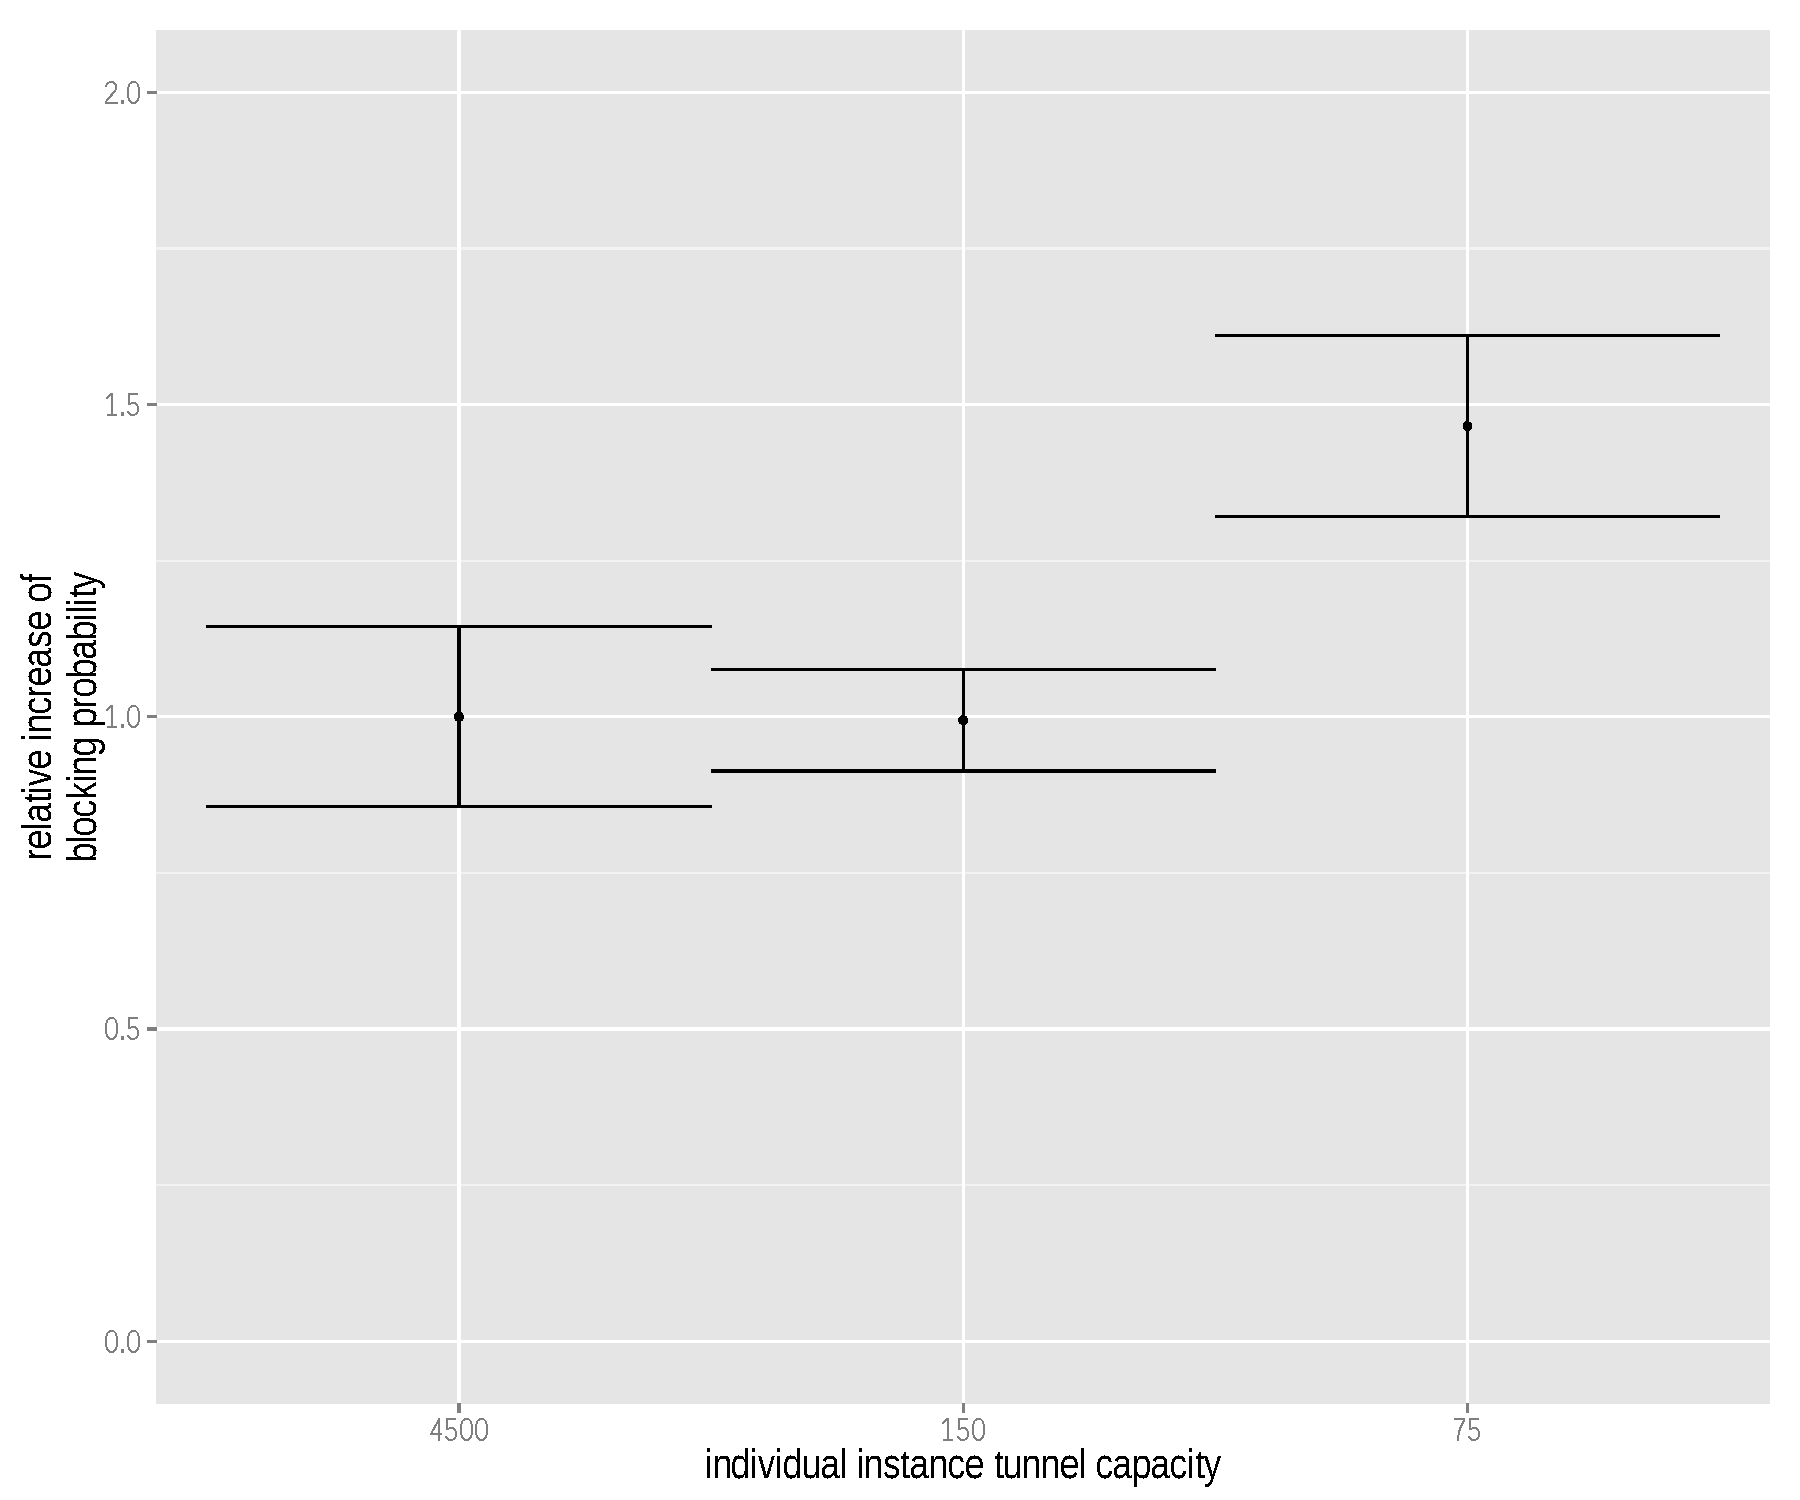
\includegraphics[width=1.0\textwidth]{images/blocking-comparison.pdf}
%   \caption{Relative increase of blocking probability on the number of servers compared to the traditional \gls{GGSN}; with the $4500$ maximum tunnels per server being on a single server, $150$ on $30$, and $75$ on $60$ servers.}
% \label{c4:fig:blocking-comparison}
% \end{figure}

%%%%%%%%%%%%%%%%%%%%%%%%%%%%%%%%%%%%%%%%%%%%%%%%%%%%%%%%%%%%%%%%%%%%%%%%%%%%%%%%
\section{Core Network Evaluation Summary}
\label{c4:sec:conclusion}

This chapter gave



 Concluding from the trace, the investigation of \gls{gtp} tunnel properties was determined to be a worthwhile measure for control plane load at the \gls{GGSN}, one of the central nodes in a \gls{3G} core network.

The investigation also showed, that the control plane is easily influenced by several device-based --- as far as they can be distinguished in a core network trace --- and time-of-day related features. The overall diurnal tunnel signaling load closely resembles the progression of the user plane. Most of the control plane's procedures are still triggered, either directly or indirectly, by user devices, of which the offered load is much smaller during night time. The trace evaluation also confirms the dominating influence of smartphones compared to other devices types, even when looking at the control plane.

But this also means, that sheer traffic volume is not a good measure to determine load, as the per-device traffic volume of a smartphone is rather low when compared to devices like pure \gls{3G} modems attached to a notebook. In this aspect, the findings also support the stories of signaling storms in mobile networks caused by applications regularly causing small amounts of network traffic. Each application interaction results in disproportionate amounts of signaling load being generated. Even worse, measures taken to improve the radio interface control plane such as Fast Dormancy could possibly have adverse effects to core signaling as they might increase the tunnel churn.

But the load investigation should not stop here. The presented approaches were just the ones that could be conducted with the available data. If one were to have access to a mobile network monitoring system or more detailed data records from such a system, it would open up many more angles in the investigation. For example, recording every individual signaling message with all \glspl{IE} would give hard numbers on the direct signaling overhead, as could measurement probes located inside the network nodes report on the CPU and memory load in order to determine the control plane's processing overhead. A closer investigation of control plane load in relation to mobility behavior should also prove very interesting, as this is one of the central motifs in every mobile network.

Learning from this historical data, queuing theoretic models were created that can describe the control plane load in such networks. These models can be easily used in network dimensioning and planning processes by means of, e.g., stationary analyses. The novel baseline control plane load model presented here is a $M(t)/G(t)/c/0$ non-stationary Erlang loss model. When used in conjunction with parameters derived from the measurement traces it can easily be used for network dimensioning. To improve scaling in the future a further \gls{GGSN} load model with features used in virtualization was also proposed.

Due to general solvability issues of non-stationary Erlang models the model is evaluated and validated using a queuing simulation in terms of their blocking and tunnel state probability as well as the general resource utilization. The virtual model provided the added benefit of being more flexible in its scaling properties and energy efficiency. This might even lead to new \gls{GGSN}-as-a-Service business models, removing the need to provide and operate large amounts of infrastructure for rare cases of peak load. 

%In the future we would like to deepen our modeling efforts to provide more dimensioning options for a core network. Also, we want to further investigate the correlation of user traffic and signaling and take a look at the implications specific traffic types bring for the core network. 

%All these investigations and modeling efforts combined could lead to a more informed approach of network planning: Being more aware of the control plane provides the necessary tools to identify probable causes for control plane activity. 

%We would also like to expand our evaluations, as there are several angles not investigated so far that could prove worthwhile. This includes an examination of the exact number and size of signaling messages flowing through the core, a more detailed picture of the processing load these messages induce at the \gls{GGSN}, and an evolved model. Furthermore, a differential analysis of our data compared to a newer dataset (potentially including \gls{LTE} access) could really prove worthwhile.

%We also look forward to searching for multiple active tunnels per device. As discussed previously, the \textit{Secondary PDP Context Activation Procedure} enables devices to establish up to ten additional tunnels attributed with a different, higher QoS level, if the network supports this. The additional load of managing and holding multiple tunnels plus the displacement of other, ``lower-quality'' traffic could prove to be an interesting investigation. Initial observations indicate that this feature is rarely used today by very few types of devices, but it will be of increased interest in the face of ongoing LTE/EPS deployments, whose specifications expand upon this secondary tunnel concept.